%=== Dissertation template borrowed from Dr. Xunwu Zuo (2021). ===%

%% UF thesis template from https://helpdesk.ufl.edu/application-support-center/etd-technical-support/ms-word-and-latex-templates/
%% LaTex template summer 2019

%=== NOTES TO FUTURE USERS ===%
% Inside ufdissertation.cls you'll find this custom environment command:
% \begin{multiFigure}
%     \centering
%     \addFigure{0.96}{path/to/fig}
%     \captionof{figure}
%         []
%         {}
%     \label{fig:X}
% \end{multiFigure}
% * Make sure that there is NOT A NEWLINE between \begin{multiFigure} and the line ABOVE it (otherwise your figs will be off-center)!

%=== Rules on CAPITALIZATION ===%
% Title Case: all principal words are capitalized except prepositions, articles, and conjunctions.
% Sentence Case: Normal sentence rules.

% Ch. 1: CHAPTER TITLES ARE ALL CAPS
% Sec. 1.2: Section Titles Are in Title Case
% Subsec. 1.2.3: Subsection Titles Are in Title Case
% Subsubsec. 1.2.3.4: Subsubsection titles are in sentence case
% Any header levels beyond subsubsections should just use bold text and should not be numbered.

\documentclass{ufdissertation}\sloppy

\usepackage[T1]{fontenc}
\usepackage{charter}
\usepackage{ragged2e} % to make text fully justified
\usepackage{tikz}%       tikz is used by almost everyone, but certainly by me for this.
\usepackage[compat=1.1.0]{tikz-feynman}% for drawing feynman diagrams 
\usepackage{pgfplots}%   pgfplots is tikz but better.
\usepackage{xspace}
\xspaceaddexceptions{]\}}
\usepackage{xcolor}
\usepackage{caption}
\usepackage{subcaption} % allowing to use subfigure inside figure
\usepackage{topcapt} % allow \topcaption
\usepackage{graphicx} % allow \resizebox
%\usepackage{amsrefs}%   amsrefs contains the .bibtex style content for mathematician papers.
\usepackage{newtxtext}
\usepackage{newtxmath}
\usepackage{mathrsfs}  % Gives fancy L for Lagrangian: \mathscr{L}
\usepackage{multirow}
\usepackage{cellspace}
\usepackage{soul}
\usepackage[greek,english]{babel}
\setlength\cellspacetoplimit{10pt}
\setlength\cellspacebottomlimit{10pt}

%=== Suz's packages for tables.
% \usepackage[margin=1in]{geometry}
% \usepackage{times}
% \usepackage[utf8]{inputenc} % seems it is by default and not needed
\usepackage{booktabs}
\newcolumntype{Y}{>{\centering\arraybackslash}X}
\newcolumntype{B}{>{\hsize=.15\hsize}Y}
\newcolumntype{M}{>{\hsize=.25\hsize}Y}
\newcolumntype{S}{>{\hsize=.05\hsize}Y}
%===

% For Suzanne's Feynman diagrams.
\usepackage{tikz}
\usetikzlibrary{patterns}
\pgfdeclarepatternformonly{south west lines}{\pgfqpoint{-0pt}{-0pt}}{\pgfqpoint{3pt}{3pt}}{\pgfqpoint{3pt}{3pt}}{
    \pgfsetlinewidth{0.4pt}
    \pgfpathmoveto{\pgfqpoint{0pt}{0pt}}
    \pgfpathlineto{\pgfqpoint{3pt}{3pt}}
    \pgfpathmoveto{\pgfqpoint{2.8pt}{-.2pt}}
    \pgfpathlineto{\pgfqpoint{3.2pt}{.2pt}}
    \pgfpathmoveto{\pgfqpoint{-.2pt}{2.8pt}}
    \pgfpathlineto{\pgfqpoint{.2pt}{3.2pt}}
    \pgfusepath{stroke}
}

%===============================%
%=== Notes on using \xspace. ===%
%===============================%
% The TeXperts (by the way, if that's not what they're called then something's wrong!)
% recommend NOT using \xspace, since once there are some cases when an extra space will be added:

% \newcommand{\words}{words\xspace}
% (\words)    % Returns: (words)
% [\words]    % Returns: [words ]
% \{\words\}  % Returns: {words }

% The author(s) of xspace didn't included ] and \} in the list of exceptions.
% If you insist on using \xspace, then simply add this to the document preamble:
% \usepackage{xspace}
% \xspaceaddexceptions{]\}}

% So what do the TeXperts recommend instead?
% They say to add `{}` to the end of every macro call:

% \newcommand{\neat}{neat}
% Some \neat words        % Returns: Some neatwords
% Some \neat{} words      % Returns: Some neat words
% Some \neat{}{}{} words  % Returns: Some neat words

% The rule in TeX is simple: after a command name that uses letters, white space is ignored.

%=================================================%
%=== Difference between the kern and the skip. ===%
%=================================================%
% In LaTeX, `\,` (backslash comma) is a thin unbreakable space, also called a 'kern'.
% It has a width of 1/6em (quite literally 1/6th the width of the 'M' in whatever font).
% On the other hand, the `~` (tilde) is a normal unbreakable space, so a little bit wider, also called a 'skip'.
% A skip is the same width of the space between words (the interword space).
% Neither kerns nor skips will be broken across lines, but ~ may get stretched: `5~Kg` -> `5    Kg`.

% Some shorthand
% turn off italics
\newcommand {\etal}{\mbox{et al.}\xspace} %et al. - no preceding comma
\newcommand {\ie}{\mbox{i.e.}\xspace}     %i.e.
\newcommand {\eg}{\mbox{e.g.}\xspace}     %e.g.
\newcommand {\etc}{\mbox{etc.}\xspace}     %etc.
\newcommand {\vs}{\mbox{vs.}\xspace}      %vs.

% Units.
% Xunwu used `\,` (a kern) at the beginning of each unit.
% I removed them.
% Jake, consider getting rid of \mbox below!
\newcommand{\gram}{\ensuremath{\text{g}}\xspace}
\newcommand{\tesla}{\ensuremath{\text{T}}\xspace}
\newcommand{\nm}{\ensuremath{\text{nm}}\xspace}
\newcommand{\mum}{\ensuremath{\mu\text{m}}\xspace}
\newcommand{\micron}{\ensuremath{\mu\text{m}}\xspace}
\newcommand{\mm}{\ensuremath{\text{mm}}\xspace}
\newcommand{\cm}{\ensuremath{\text{cm}}\xspace}
\newcommand{\meter}{\ensuremath{\text{m}}\xspace}
\newcommand{\km}{\ensuremath{\text{Km}}\xspace}
\newcommand{\ns}{\ensuremath{\text{ns}}\xspace}
\newcommand{\mus}{\ensuremath{\mu\text{s}}\xspace}
\newcommand{\ms}{\ensuremath{\text{ms}}\xspace}
\newcommand{\snd}{\ensuremath{\text{s}}\xspace}
\newcommand{\TeV}{\ensuremath{\mbox{TeV}}\xspace}
\newcommand{\GeV}{\ensuremath{\mbox{GeV}}\xspace}
\newcommand{\MeV}{\ensuremath{\mbox{MeV}}\xspace}
\newcommand{\pb}{\ensuremath{\mbox{pb}}\xspace}
\newcommand{\fb}{\ensuremath{\mbox{fb}}\xspace}
\newcommand{\invfb}{\ensuremath{\mbox{fb}^{\scriptscriptstyle -1}}\xspace}
\newcommand{\lumi}{\ensuremath{\mathcal{L}}\xspace}

% analysis tools
\newcommand{\GEANTfour} {{\textsc{Geant4}}\xspace}
\newcommand{\HERWIGpp}{{\textsc{HERWIG++}}\xspace}
\newcommand{\HERWIGSeven}{{\textsc{HERWIG7}}\xspace}
\newcommand{\MADGRAPH} {\textsc{MadGraph}\xspace}
\newcommand{\MCATNLO} {\textsc{mc@nlo}\xspace}
\newcommand{\POWHEG} {{\textsc{powheg}}\xspace}
\newcommand{\PYTHIA} {{\textsc{pythia}}\xspace}
\newcommand{\SHERPA} {{\textsc{sherpa}}\xspace}
\newcommand{\MCFM} {{\textsc{mcfm}}\xspace}
\newcommand{\TOPpp} {{\textsc{TOP++}}\xspace}
\newcommand{\MGvATNLO} {\MADGRAPH{}5\_a\MCATNLO}
\newcommand{\FEWZ} {{\textsc{fewz}}\xspace}

% physics variables
\newcommand{\pt}{\ensuremath{p_{\mathrm{T}}}\xspace}
\newcommand{\ET}{\ensuremath{E_{\mathrm{T}}}\xspace}
\newcommand{\HT}{\ensuremath{H_{\mathrm{T}}}\xspace}
\newcommand{\MET}{\ensuremath{E_{\mathrm{T}}^{\text{miss}}}\xspace}
\newcommand{\MHT}{\ensuremath{H_{\mathrm{T}}^{\text{miss}}}\xspace}
\newcommand{\MT}{\ensuremath{M_{\mathrm{T}}}\xspace}
\newcommand{\abseta}{\ensuremath{\left| \eta \right|}\xspace}

% particles
\newcommand{\Pn}{\ensuremath{\mathrm{n}}}
\newcommand{\Pp}{\ensuremath{\mathrm{p}}}
\newcommand{\PV}{\ensuremath{\mathrm{V}}\xspace}
\newcommand{\PW}{\ensuremath{\mathrm{W}}\xspace}
\newcommand{\PZ}{\ensuremath{\mathrm{Z}}\xspace}
\newcommand{\PH}{\ensuremath{\mathrm{H}}\xspace}
\newcommand{\Pe}{\ensuremath{\mathrm{e}}\xspace}
\newcommand{\Pg}{\ensuremath{\mathrm{g}}\xspace}
\newcommand{\Pq}{\ensuremath{\mathrm{q}}\xspace}
\newcommand{\Paq}{\ensuremath{\overline{\Pq}}\xspace}
\newcommand{\Pqb}{\ensuremath{\mathrm{b}}\xspace}
\newcommand{\Paqb}{\ensuremath{\overline{\Pqb}}\xspace}
\newcommand{\Pqt}{\ensuremath{\mathrm{t}}\xspace}
\newcommand{\Paqt}{\ensuremath{\overline{\Pqt}}\xspace}
\newcommand{\PGn}{\ensuremath{\nu}\xspace} % generic neutrino
\newcommand{\PAGn}{\ensuremath{\overline{\nu}}\xspace} % generic neutrino

%=== Particle combos. ===%
\newcommand{\pp}{\ensuremath{\mathrm{pp}}\xspace}
\newcommand{\ee}{\ensuremath{\mathrm{e^+ e^-}}\xspace}
\newcommand{\fourell}{\ensuremath{4\ell}\xspace}
\providecommand{\ttH}{\ensuremath{\Pqt\Paqt\PH}\xspace}
\providecommand{\ggH}{\ensuremath{\Pg\Pg\PH}\xspace}
\providecommand{\qqH}{\mbox{VBF}\xspace}
\providecommand{\ZH}{\ensuremath{\PZ\PH}\xspace}
\providecommand{\WH}{\ensuremath{\PW\PH}\xspace}
\providecommand{\VH}{\ensuremath{\PV\PH}\xspace}
\providecommand{\bbH}{\ensuremath{\Pqb\Paqb\PH}\xspace}
\providecommand{\tHq}{\ensuremath{\Pqt\PH\Pq}\xspace}
\providecommand{\tHW}{\ensuremath{\Pqt\PH\PW}\xspace}
\providecommand{\qqZH}{\ensuremath{\Pq\Pq\PZ\PH}\xspace}
\providecommand{\ggZH}{\ensuremath{\Pg\Pg\PZ\PH}\xspace}
\providecommand{\DY}{\mbox{DY}\xspace}
\providecommand{\ttbar}{\ensuremath{\Pqt\Paqt}\xspace}
\providecommand{\ggZZ}{\ensuremath{\Pg\Pg\PZ\PZ}\xspace}
\providecommand{\WZ}{\ensuremath{\PW\PZ}\xspace}
\providecommand{\ZZ}{\ensuremath{\PZ\PZ}\xspace}
\providecommand{\VVV}{\ensuremath{\PV\PV\PV}\xspace}

\newcommand{\Vjets}{\ensuremath{\PV\text{+jets}}\xspace}
\newcommand{\Zee}{\ensuremath{\PZ(\Pe\Pe)}\xspace}
\newcommand{\Zll}{\ensuremath{\PZ(\ell\ell)}\xspace}
\newcommand{\Zvv}{\ensuremath{\PZ(\nu\overline{\nu})}\xspace}
\newcommand{\Zmmjets}{\ensuremath{\PZ(\mu\mu)\text{+jets}}\xspace}
\newcommand{\Zlljets}{\ensuremath{\PZ(\ell\ell)\text{+jets}}\xspace}
\newcommand{\Zjets}{\ensuremath{\PZ\text{+jets}}\xspace}
\newcommand{\DYjets}{\ensuremath{\PZ/\gamma^{*}\text{+jets}}\xspace}
\newcommand{\tZq}{\ensuremath{\Pqt\PZ\Pq}\xspace}
\newcommand{\tZW}{\ensuremath{\Pqt\PZ\PW}\xspace}

\newcommand{\kappaz}{\ensuremath{\kappa\smash[b]{^{\PGn\PAGn}}}\xspace}
\newcommand{\kappaV}{\ensuremath{\kappa_{\mathrm{V}}}\xspace}
\newcommand{\kappaF}{\ensuremath{\kappa_{\mathrm{F}}}\xspace}
\newcommand{\kappazi}{\ensuremath{\kappa_{i}\smash[b]{^{\PGn\PAGn}}}\xspace}

% Reactions/Processes.
\newcommand{\hmm}{\ensuremath{\PH \to \mu\mu}\xspace}
\newcommand{\zmm}{\ensuremath{\PZ \to \mu\mu}\xspace}
\newcommand{\hzzfourl}{\ensuremath{\PH \to \PZ\PZ \to 4\ell}\xspace}

%=== RedBkg ===%
\newcommand{\looselep}{\ensuremath{\ell_{\mathrm{L}}}\xspace}
\newcommand{\ZplusL}{\ensuremath{\PZ + \looselep}\xspace}
\newcommand{\ZplusX}{\ensuremath{\PZ + \mathrm{X}}\xspace}
\newcommand{\Zplusjets}{\ensuremath{\PZ + \text{jets}}\xspace}
\newcommand{\WZplusjets}{\ensuremath{\WZ + \text{jets}}\xspace}
\newcommand{\Zgammastar}{\ensuremath{\PZ/\gamma^*}\xspace}
\newcommand{\ttbarplusjets}{\ensuremath{\Pqt\Paqt + \text{jets}}\xspace}
\newcommand{\twoPtwoFexp}{\ensuremath{N_{\mathrm{2P2F}}}\xspace}
\newcommand{\threePoneFexp}{\ensuremath{N_{\mathrm{3P1F}}}\xspace}
\newcommand{\fourPexp}{\ensuremath{N_{\mathrm{4P}}^{\mathrm{RB}}}\xspace}
\newcommand{\threePoneFzz}{\ensuremath{N_{\mathrm{3P1F}}^{\ZZ}}\xspace}
\newcommand{\threePoneFzztilde}{\ensuremath{\tilde{N}_{\mathrm{3P1F}}^{\ZZ}}\xspace}
\newcommand{\threePoneFobs}{\ensuremath{N_{\mathrm{3P1F}}^{\mathrm{obs}}}\xspace}
\newcommand{\twoPtwoFobs}{\ensuremath{N_{\mathrm{2P2F}}^{\mathrm{obs}}}\xspace}
\newcommand{\effprpass}{\ensuremath{\epsilon^{\mathrm{pr}}_\mathrm{P}}\xspace}
\newcommand{\effprfail}{\ensuremath{\epsilon^{\mathrm{pr}}_\mathrm{F}}\xspace}
\newcommand{\effnppass}{\ensuremath{\epsilon^{\mathrm{np}}_\mathrm{P}}\xspace}
\newcommand{\effnpfail}{\ensuremath{\epsilon^{\mathrm{np}}_\mathrm{F}}\xspace}
\newcommand{\qqZZfourl}{\ensuremath{\mathrm{q\bar{q} \to ZZ \to 4\ell}}\xspace}
\newcommand{\ggZZfourl}{\ensuremath{\mathrm{gg \to ZZ \to 4\ell}}\xspace}
\newcommand{\qqggZZfourl}{\ensuremath{\mathrm{q\bar{q}/gg \to ZZ \to 4\ell}}\xspace}

\newcommand{\mmm}{\ensuremath{m_{\mu\mu}}\xspace}
\newcommand{\mll}{\ensuremath{m_{\ell\ell}}\xspace}
\newcommand{\mjj}{\ensuremath{m_{\mathrm{jj}}}\xspace}
\newcommand{\brhmm}{\ensuremath{{\mathcal{B}(\PH \to \mu\mu)}}\xspace}
\newcommand{\brhff}{\ensuremath{{\mathcal{B}(\PH \to f\overline{f})}}\xspace}
\newcommand{\detajj}{\ensuremath{\Delta\eta_{\mathrm{jj}}}\xspace}
\newcommand{\dphijj}{\ensuremath{\Delta\phi_{\mathrm{jj}}}\xspace}
\newcommand{\NNPDF} {\textsc{nnpdf}\xspace}
\newcommand{\dzeroPV}{\ensuremath{\text{d0}_{\text{PV}}}\xspace}
\newcommand{\dzeroBS}{\ensuremath{\text{d0}_{\text{BS}}}\xspace}
\newcommand{\dptoverptsquare}{\ensuremath{(\pt^{Roch} - \pt^{Gen})/\pt^2}\xspace}
\newcommand{\mh}{\ensuremath{m_{\PH}}\xspace}

\newcommand{\SoB}{\ensuremath{S/B}\xspace}

\newcommand{\RochCorr}{\textit{Rochester correction}\xspace}
\newcommand{\FSR}{\textit{FSR recovery}\xspace}
\newcommand{\GeoFit}{\textit{GeoFit correction}\xspace}

%=== N.B.: If you want to use biblatex, go into ufdissertation.cls and search for 'biblatex' (un)comment instructions.
% \usepackage[sorting=none, backend=biber, style=phys, biblabel=brackets]{biblatex}
% \usepackage[sorting=none]{biblatex}
% \addbibresource{biblatex-phys.bib}  % If using biblatex: uncomment this.

% Enable format for table, figure, object
\haveTablestrue%        Uncomment this if you have tables in your thesis.
\haveFigurestrue%       Uncomment this if you have figures in your thesis.
%\haveObjectstrue%       Uncomment this if you have Objects in your thesis. This is almost certainly not the case however.

%%%%%%%%%%%%%%%%%%%%%%%%%%%%%%%%%%%%%%%%%%%%%%%%%%%%%%%%%%%%%%%%%%%%%%%%%%%%%%%%
%%% Below are the commands to set the degree type, department, graduation time, and chair. 
%       Most of these are self explanatory. 
%       Note: The \chair command takes an optional argument for a cochair. 
%           So if John was your chair and Jacob was a cochair, you would use \chair[Jacob]{John}.
%           If John was your chair and you had no cochair, you can simply use \chair{John}.
%%%%%%%%%%%%%%%%%%%%%%%%%%%%%%%%%%%%%%%%%%%%%%%%%%%%%%%%%%%%%%%%%%%%%%%%%%%%%%%%
% Author info
\title{Precision Measurement of the Higgs Boson Mass and Search for Dilepton Mass Resonances in $\htofourl$ Decays Using the CMS Detector at the LHC}
\degreeType{Doctor of Philosophy}         % Official name of your degree; eg "Doctorate of Philosophy".
\major{Physics}                              % Your official Department.
\author{Jake Rosenzweig}%                  Your Name
\thesisType{Dissertation}%              Dissertation (PhD) or Thesis (Masters)
\degreeYear{2022}%                      Intended graduation year (not the year you submit the thesis)
\degreeMonth{December}%                   Month of graduation should be May, August, or December.
\chair[Guenakh Mitselmakher]{Andrey Korytov}%                   Chair and Cochair (see comment block above).

%% additional sections
% \setDedicationFile{tex/dedicationFile}%                Dedication Page
% \setAcknowledgementsFile{tex/acknowledgementsFile}%    Acknowledgements Page
% \setBiographicalFile{tex/biographyFile}%               Biography file of the Author (you).
% \setAbstractFile{tex/abstractFile}%                    Abstract Page (This should only include the abstract itself)

%=== Bibliography is printed in the command \setReferenceFile below. ===%
% \bibliographystyle{plain}
% \bibliography{referenceFile}
\setReferenceFile{referenceFile}{jhep}%        References. First argument is your bibtex source file (.bib) the second argument is your bibtex style file (.bst).
% \setReferenceFile{referenceFile}{amsplain}
% Use the style "unsrtnat" since it sorts references in cite order and shows url.
% Other bibliographystyles: unsrtnat, apsrev, ieeetr, jhep (beautiful but doesn't show url).

%%%% These are NOT required, so only use them if you actually need/have them.
% \setAbbreviationsFile{tex/abbreviations}%           Abbreviations Page. Jake changed this to say "LIST OF ACRONYMS".
% \setAppendixFile{tex/appendix}%                     Appendix Content; hyperlinking might be weird. TODO: Fix hyperlinking.
% \multipleAppendixtrue%                          Uncomment this if you have more than one appendix, otherwise leave it commented. This adds "A", "B" in the TOC next to each Appendix entry.

%=== Main Text ===%
\begin{document}
%%%%%%%%%%%%%%%
%--- Intro ---%
%%%%%%%%%%%%%%%
% \chapter{Introduction}

The universe has particles.
The interactions between these particles are described very well by the Standard Model (SM).
However, the SM doesn't predict the masses of particles.
In 1964, the Brout-Englert-Higgs mechanism proposed that breaking the electroweak gauge symmetry of the vacuum would give rise to non-zero masses of the weak gauge bosons.
This would yield a secondary effect too:
there should exist a fundamental scalar boson which is the quantum of the so-called ``Higgs field''.
On July 4th, 2012, this Higgs boson was discovered.


At first glance, the universe appears to be an overwhelmingly vast and complicated place.
However upon closer inspection, it is comprised of only a few different kinds of fundamental particles.
Particle physics has given rise to the Standard Model (SM) which mathematically describes these constituents and their interactions with each other.




The Standard Model (SM) is an impressively accurate mathematical theory which describes the fundamental particles of the universe and the rules for their possible interactions.
Problematically though, the SM predicts that all particles are massless.


Get to the Higgs boson.

Why is it important?
Knowing the mass of the Higgs boson 





% The Universe is comprised of just a few basic building blocks: the fundamental particles.

% By understanding the rules by which these particles interact, we can ;
% this is the aim of the Standard Model (SM) of Particle Physics. 

%  are described mathematically by the impressively accurate Standard Model (SM) of Particle Physics.

% Although there are four fundamental forces of nature, the SM takes into account three of the four forces in nature:

%%%%%%%%%%%%%%%%%%%%%%%%
%--- Standard Model ---%
%%%%%%%%%%%%%%%%%%%%%%%%
% \chapter{Theory}
\label{ch:theory}

\section{The Standard Model}
\label{sec:sm}



\begin{itemize}
    \item strong force $(1)$
    \item EM force $(10^{-1})$
    \item weak force $(10^{-6})$
    \item gravitational force $(10^{-40})$
\end{itemize}
Speaking of forces, the four fundamental forces found in nature, along with their decreasing, relative strength are: 


\subsection{Electroweak Interaction}
\label{subsec:ew_inter}

\subsection{Strong Interaction}
\label{subsec:strong_inter}

\subsection{Higgs Mechanism}
\label{subsec:higgs_mech}

%%%%%%%%%%%%%
%--- LHC ---%
%%%%%%%%%%%%%
% % TODO: Maybe in the \caption[], don't use a final period at the end within the square brackets? Check TOC.
% Great animation about protons going through the CERN accelerator complex.
% https://www.youtube.com/watch?v=FLrEghnKncA
\chapter{THE LARGE HADRON COLLIDER}
\label{ch:lhc}

% OUTLINE
% \section{Motivation for a Large Hadron Collider}
\section{Motivation}
Although the SM
% TODO:(Chapter~\ref{ch:theory})
has shown to be an astoundingly accurate framework so far, it must continue to be scrutinized by the barrage of measurements that either confirm or contradict its predictions.
% cross-examined
Interestingly, a recent measurement of the mass of the \PW boson has shown significant deviation from SM predictions, with a sensitivity of 7$\sigma$~\cite{cdf_collaboration_high-precision_2022}.
After all, undeniable fact comes from reproducible results obtained from measurement---not from some theoretical model which \emph{may} or \emph{may not} describe reality.
Whenever results from measurement contradict the predictions made by a model, the model must necessarily be cast aside and replaced by one whose predictions are in alignment with truth, \ie \emph{measurement}.
% the truth of Nature

So how \emph{are} measurements obtained in the realm of particle physics?
% be continuously tested for its accuracy.
% Must be shaken by the results of experiment to see if its foundation is stable.
% So far, it has upheld against the onslaught of measurements but must be continuously tested for accuracy.
% , it does not explain many phenomena observed in the universe, as discussed in ().
% Although the SM (Chapter~\ref{ch:theory}) is an astoundingly accurate framework, it does not explain many phenomena observed in the universe, as discussed in ().
% As discussed in TODO:PROBLEMS WITH SM, there is observed physics that has not yet been explained in a coherent theoretical and mathematical framework.
% There are currently many searches for physics \emph{beyond the standard model} (BSM) which may explain certain observed physical phenomena that .
% robust, elegant, and accurate (so far), 
% perhaps there is physics beyond the SM (BSM).
% After all, the truth of Nature comes from the results of measurements---not from mathematical and theoretical models.
% Although the standard model (SM) of particle physics  is rather elegant
% and  for the physical phenomena that it does explain.
Modern day physicists study the fundamental constituents of matter and their interactions by using state-of-the-art technologies combined with time-tested methodologies:
%  is to do it the same way humans have been doing it for centuries:
by smashing tiny bits of matter together to turn them into even \emph{tinier} bits.
Such is the purpose of the world's largest and most powerful particle accelerator---the Large Hadron Collider (LHC).

\section{The LHC at CERN}
% The circular LHC ring straddles the Franco-Swiss border, approximately 100\meter below the surface of the earth
% (Fig.~\ref{fig:lhc_and_boosters}, Left).
% The ring itself has a circumference of 26.7\Km, making its inscribed area (56.7$\Km^{2}$) almost four times greater than the area of the neighboring city of Geneva (15.9$\Km^{2}$).
% This machine is not only a particle accelerator but also a proton--proton (\pp) collider, sending one beam of protons travelling clockwise and the other beam counterclockwise around the ring. 
Deep beneath the surface of the earth (50--175\meter), the LHC straddles the border shared by France and Switzerland.
Sandwiched between the scenic Jura mountains to the northwest and the sprawling city of Geneva (French: Genève) to the southeast is CERN.
To illustrate the enormous circumference (26.659\Km) of this circular accelerator, Fig.~\ref{fig:lhc_on_map_and_complex} (Left) shows the LHC drawn on a map. % TODO:UPDATE WITH A,B
% Map and CERN complex.
%%%%%%%%%%%%%%%%%%%%
\begin{figure}[pbth]
    \centering
    \includegraphics[width=0.48\textwidth,keepaspectratio]{figures/lhc/lhc_drawn_on_map_withpoints.png}
    \includegraphics[width=0.48\textwidth,keepaspectratio]{figures/lhc/cern_complex.png}
        \caption
            [(Left) A map image of the LHC ring. (Right) The CERN accelerator complex]
            {TODO:Break these images up into 2 separate images. (Left) The LHC ring (bigger ring) and the Super Proton Synchrotron (smaller ring) with the nearby town of Geneva for size comparison. 
            The four red stars indicate the \pp collision points. 
            (Right) The accelerator complex at CERN.
            } 
        \label{fig:lhc_on_map_and_complex}
    \end{figure}
%%%%%%%%%%%%%%%%%%%%
For reference, the inscribed area of the LHC (56.7$\Km^{2}$) is almost four times greater than the area of the neighboring city of Geneva (15.9$\Km^{2}$).

The LHC is not only a particle \emph{accelerator} but also a proton--proton (\pp), proton--lead ion, and lead--lead ion \emph{collider}.
By sending one particle beam clockwise around the ring and the other beam counterclockwise, the charged particles are carefully maneuvered using dipole magnets and tightly collimated using quadrupole magnets before they ultimately collide at 4 specific points along the LHC, as shown in Fig.~\ref{fig:lhc_on_map_and_complex} (Left, red stars).
% , anywhere from , , and sandwiched between the scenic Jura mountains to the west and the sprawling city of Geneva (Genève) to the east
%  straddles the Franco-Swiss border, approximately 100\meter below the surface of the earth (Fig.~\ref{fig:lhc_and_boosters}, Left).
When the LHC is fully powered, \emph{each} proton in the beam carries an average energy of 6.5\TeV which gives a single \pp collision a massive center-of-mass energy of 13\TeV\footnote{
    For comparison, a \emph{mosquito} in flight carries about 13\TeV of kinetic energy.
    For two \emph{fundamental particles} to collide with this much energy is truly astonishing!
}.
This emulates the conditions theorized to exist at the beginning of the universe, which allows cosmological studies to be carried out.
The hugely energetic \pp collisions cause the quark and gluon constituents within the protons to interact with each other and transform into new particles.
The newly created particles and the residual particle debris are ejected away from the collision point---whether straight down the beampipe, completely orthogonal to it, or somewhere in between.
Massive particle detectors are stationed at each of the 4 collision points to detect the outgoing particle ``spray''.
The 4 main particle detectors and their locations along the LHC are:
\begin{itemize}
    \item A Toroidal LHC ApparatuS (ATLAS)---located at the first collision point (P1)
    \item A Large Ion Collider Experiment (ALICE)---located at P2
    \item the Compact Muon Solenoid (CMS, Chapter~\ref{ch:cms}) experiment---located at P5
    \item the LHC-beauty (LHCb) experiment---located at P8
\end{itemize}
% TODO: Get rid of extra newline that appears after itemize.
% ATLAS	A Toroidal LHC Apparatus
% CMS	Compact Muon Solenoid
% LHCb	LHC-beauty
% ALICE	A Large Ion Collider Experiment
% TOTEM	Total Cross Section, Elastic Scattering and Diffraction Dissociation
% LHCf	LHC-forward
% MoEDAL	Monopole and Exotics Detector At the LHC
% FASER	ForwArd Search ExpeRiment
% SND	Scattering and Neutrino Detector
The world-renowned feat of digging the tunnel for, constructing, commissioning, and monitoring the LHC was made possible by CERN:
% - Before the LHC, LEP was originally in the tunnel.
%     - LEP ran from TODO--TODO.
the European Organization for Nuclear Research (French: \emph{Conseil Européean pour la Recherche Nucléaire}).
CERN is an international collaboration of---at the time of this writing---more than 33 countries,
% it's actually 34.
% Learn about the series of accelerators here:
% https://cdsweb.cern.ch/record/2771424/files/CERNAnnualReport_2020_EN.pdf
each of which is considered either a Member State, an Associate Member State, or an Observer.
The complex of CERN (Fig.~\ref{fig:lhc_on_map_and_complex}, Right) is located just to the west of P1 and is akin to a small science \emph{city}---complete with many offices, manufacturing facilities, and experiments such as the Antiproton Decelerator (AD), the Neutrons Time of Flight (n$\_$TOF), and the Isotope Separator OnLine (ISOLDE) experiments.
% the world's largest and most powerful particle accelerator, the Large Hadron Collider (LHC).
% The completion of this world-renowned feat was only possible through the careful efforts of thousands of scientists, engineers, administrators, \etc from all over the world.
% At the time of this writing, CERN is associated with at least 33 countries, each of which is considered either a Member State, an Associate Member State, or an Observer.
Although the LHC is the most famous of the accelerators at CERN, its fame is only made possible by a series of smaller and lesser-known accelerators that \emph{feed} the LHC.
% would not be able to accelerate \emph{any} charged particles from rest; not collide particles at such massive energies if not for the lesser-known accelerators that feed into the LHC.
% but it takes clever engineering and a series of smaller accelerators to eventually feed particles into the LHC to reach their maximum energy of 6.5\TeV.
Therefore, a natural way to explore the intricacies and inner workings of the LHC is to follow the path of one of its ``inhabitants''---a single proton---as it makes its way to and through the gigantic collider.

\section{The Journey of a Proton at the LHC}
The journey to discovery begins in a surprisingly small tank of hydrogen gas (\htwo) located in the LINAC4 building at the main CERN site.
% , in which a proton that is bound to another proton as a molecule of H2 .
% Pic of hydrogen source from here: https://www.lhc-closer.es/taking_a_closer_look_at_lhc/0.linac4
Inside this tank, a proton---conveniently named Paul Roton, or just \pname for short---and $\mathcal{O}(10^\text{23})$ other protons (TODO:DOUBLE CHECK THIS)
% TODO: fix: $1\tentothe{11}$
coexist in bound states as molecules of H$_2$.
Although the tank has a meager mass of 
% TODO\Kg,
$\approx$10\Kg,
it has enough protons inside to keep the LHC colliding protons for over \emph{200\,000 years} of constant operation.

\pname and the rest get injected into a series of increasingly larger and more powerful accelerators.
They begin their journey at the \emph{Linac4}---a linear particle accelerator---that converts the particles into hydride ions (H$^-$) and then accelerates them to 160\MeV, at which point, they are fed into the \emph{Proton Synchrotron Booster} (PSB).
In the PSB, each H$^-$ has its electron pair completely stripped away, leaving only the bare proton ($\Pp^+$).
\pname then enters a series of circular accelerators, where each machine feeds its protons into the next in order to increase the proton center-of-mass energy by at least 1 order of magnitude with each feeding.
The flow of accelerators is as follows:
\begin{itemize}
    % TODO: mention electric field?
    % \item The flow 
    \item From the PSB, \pname are the rest are accelerated to 2\GeV and then injected into the \emph{Proton Synchrotron} (PS).
    \item The PS increases the energy of the particles to 26\GeV and then feeds the protons into the \emph{Super Proton Synchrotron} (SPS).
    \item Next, the SPS energizes the protons to a center-of-mass energy of 450\GeV and sends bunches of protons (so-called \emph{proton bunches}, $\approx$$10^\text{11}$ protons) into the LHC. % TODO: change \tentothe -> \timestentothe %  are packed together into a ``proton bunch''. % a accelerates protons to com energy
\end{itemize}
% TODO: Mention: A single proton bunch is about the size of a human hair ($\approx$50\mum wide and $\approx$10\cm long). 
% TODO: Mention: The clockwise and counterclockwise rings are filled to a maximum of 2808 proton bunches, each one spaced 25\ns apart, and then sent to collide. 
It is inside the LHC that \pname and its fellow protons within its proton bunch are given precisely timed \emph{kicks} by the electric field\footnote{
    The electric field quickly oscillates between pointing parallel to the direction of travel of the proton bunch to pointing \emph{antiparallel} to the direction of travel.
    Therefore, precise timing is required to ensure that the electric field only points parallel so as to speed up the protons in the proton bunch.
    This is analgous to the timing required when pushing a person on a swing:
    the pusher must push at \emph{just} the right time to increase the momentum of the one swinging, lest the pusher slows the swinger down!
} within radio-frequency (RF) cavities.
After sufficient energy is delivered to the proton bunches, they finally achieve their max speed of 0.999\,999\,96$c$. %   99.999\,996\%$c$.
At this speed, \emph{each proton} in the proton bunch carries a center-of-mass energy of 6.5\TeV.

\pname and its neighboring protons in the proton bunch are nearly ready for a head-on collision with another proton bunch to make interesting physics.
The only problem is that the proton bunches must be turned (to keep them in the circular LHC) and must be tightly squeezed down (to increase the chance of \pp collisions).
Since the protons are bare, they are all positively charged, and are subject to a Lorentz force when they pass through a magnetic field.
Therefore, the LHC is equipped with 1232 dipole magnets distributed all along its circumference to turn the proton bunches.
The cross section of such a dipole magnet is shown in Fig.~\ref{fig:lhc_dipole_xs}.
Each dipole magnet is 14.3\meter long, weighs 35\tonne, costs nearly 500\,KCHF to produce, and has nearly 11\,700\,A of current running through it.  % TODO: make command for amps unit?
Only with such massive currents is it possible to generate the appropriate magnetic field strength of 8\tesla to keep the protons moving in a circular fashion at their near-light speed. 
The magnetic field is maintained by copper-clad niobium-titanium coils, which requires the cryogenics conditions of 96\tonne of superfluid helium-4 to achieve the necessary temperature of 1.9\kelvin to reach a superconducting state; 
this temperature is colder than that of outer space.
% TODO: Check numbers here and ref.
There are also 506 quadrupole magnets (TODO:CITE) that compress the proton bunches as tightly as possible before collision with the other oncoming proton beam.
%%%%%%%%%%%%%%%%%%%%
\begin{figure}[pbth]
\centering
\includegraphics[width=15cm,height=10cm,keepaspectratio]{figures/lhc/lhc_dipole_xs.jpg}
    \caption
        [Cross section of an LHC dipole magnet.]
        {A cross section of one of the 1232 dipole magnets which span the entire length of the LHC tunnel.} 
    \label{fig:lhc_dipole_xs}
\end{figure}
%%%%%%%%%%%%%%%%%%%%

% As two bunches (one from the clockwise proton beam and the other from the counterclockwise beam) approach one of the four detector points along the LHC, each bunch is squeezed tightly using quadrupole magnets, helping to focus the beams which increases the chance for the desired \pp collisions.
As the two proton beams approach one of the four detector points along the LHC, two of the oncoming bunches are squeezed tightly using the quadrupole magnets which increases the chance for the desired \pp collisions.
During a bunch crossing (BX), amazingly most of the protons just pass right by one another; 
out of the $\approx$$10^\text{11}$ possible \pp collisions that could have occurred, Fig.~\ref{plt:pileup} shows that on average only approximately 32 collisions occurred per BX during the 2018 Run of the LHC. %, according to a particle detector called CMS, described in Chapter~\ref{ch:cms}.  a mere 50 collisions take place on average (\ie only 0.0001\%).
This is a testament to just how small protons truly are.
%from 50 $\mu$m
In the event that \pname does not collide with any of the oncoming protons, then it is simply ``recycled'' and continues going around the LHC ring for another opportunity at a \pp collision.
When the anticipated moment finally comes---\ie a ``hard'' \pp collision is realized, as shown in Fig.~\ref{fig:pp_collision}---the energy of the single collision contains a monstrous center-of-mass energy of $\sqrt{s} = 13\TeV$, which is more than enough to create new particles like top quarks, Higgs bosons (Chapter~\ref{ch:higgs_mass}), and potentially BSM particles (Chapter~\ref{ch:dilep_res}).
% Truly, it is the particles inside the protons, the so-called \emph{partons} that interact with one another, as shown in Fig.~\ref{fig:pp_collision}.
%%%%%%%%%%%%%%%%%%%%
\begin{figure}[h]
    \centering
    \includegraphics[width=0.7\textwidth,keepaspectratio]{figures/lhc/pileup_pp_2018.png}
        \caption
            [Distribution of the average pile up during the LHC 2018 run.]
            {Histogram showing the distribution of the average number of \pp collisions per proton bunch crossing (pile up) which CMS recorded during the LHC 2018 run.} 
        \label{plt:pileup}
    \end{figure}
    %%%%%%%%%%%%%%%%%%%%
In order to analyze such interesting particles, one needs to detect the outgoing particles produced from the \pp collisions.
One such dedicated particle detector is located at Point 5---the Compact Muon Solenoid (CMS) detector---and is described in the next chapter.
    %%%%%%%%%%%%%%%%%%%%
\begin{figure}[h]
    \centering
    \includegraphics[width=0.7\textwidth,keepaspectratio]{figures/lhc/proton_proton_quarksandgluons.jpg}
        \caption
            [Diagram showing the constituents (\emph{partons}) of two protons interacting in a \pp collision.]
            {Two protons can be smashed together at very high energies to have their constituent partons interact and convert their high energies into new kinds of matter.} 
        \label{fig:pp_collision}
    \end{figure}
    %%%%%%%%%%%%%%%%%%%%

% Finally two incoming proton bunches approach a common collision point.
% - Frequency of BX: considering that proton bunches are spaced 25\ns apart, this means 

% TODO: FCC?
% Just as the PS feeds protons into the SPS, which feeds protons into the LHC, so too is it being considered for the LHC to feed a new project---the 100\Km Future Circular Collider.

% TODO:
% SPECS
% - Luminosity
% - rates
% - data

% N obs events = xs * eff * Lint 
% cross section is specific to the process
% efficiency is ideally unity.


% LPS SPS
% into a beam pipe going clockwise and another 2800 bunches going around counterclockwise, 




% TODO:
% \subsection{Physics of the LHC}
% The luminosity of the LHC is $\mathcal{O}(\LHigh)$ the number of particles 
% It should be mentioned that the luminosity of the LHC is on the order of \LHigh. %$10^{34}$ Hz/cm$^2$.




% The LHC has ushered in the era of ``TeV-scale physics'',
% exploring the 
% - which is about the same amount of energy of a really fat flying mosquito.

% It takes a proton \~90 $\mu$s 
% to make a complete revolution around the LHC moving at such a speed.

% The LHC collides particles using the brightest beams and highest energies that humans have ever made.
% Bright beams meaning highest luminosity.

% Higgs boson produced every 1 billion collisions.

% Beginning in 2026 (FIXME), the LHC will undergo a ``Phase 2'' upgrade and become the High-Luminosity LHC.
% This upgrade will increase the collider's luminosity by 10 fold (FIXME) and is predicted to deliver SO much data 3000 fb?.

% TODO:
% \section{High-Luminosity LHC}

%%%%%%%%%%%%%
%--- CMS ---%
%%%%%%%%%%%%%
% \chapter{THE CMS DETECTOR} 
\label{ch:cms_detector}
%%%%%%%%%%%%%%%%%%%%
\begin{figure}[pbth]
\centering
\includegraphics[width=10cm,height=10cm,keepaspectratio]{figures/cms/cms_poster_SX5.jpg}
    \caption{
    Life-size poster of the CMS detector, taken during CERN Open Days 2019
    in the SX5 warehouse where parts of CMS were assembled.}
    \label{fig:cms_poster}
\end{figure}
%%%%%%%%%%%%%%%%%%%%
Weighing in at 14,000 tonnes, standing 5 stories tall (15 m), and reaching 29 m long, the Compact Muon Solenoid (CMS) experiment is one of two general-purpose particle detectors at the LHC (Fig.~\ref{fig:cms_poster}).
CMS is situated approximately 100 m under the earth at the fifth collision point (Point 5) along the LHC (Fig.~\ref{fig:lhc_points}).
In 2012, both CMS and its competing experiment, ATLAS, independently discovered the Higgs boson.

% The purpose of CMS is to precisely measure the kinematical properties of the abundant decay products that come from the \pp collisions delivered by the LHC.
% These particle properties, like momentum, energy, and charge, are used to reconstruct the particle trajectories (``tracks'') and help to identify the particles themselves.
As discussed in Section (TODO: REF), the LHC collides bunches of protons every 25 ns to produce thousands of new particles which then travel away from the interaction point.
CMS is built around the interaction point in a series of cylindrical subdetectors for nearly hermetic coverage so that most of the particles must travel through CMS.
The detector sports a solenoid, after which CMS was named, which generates a 3.8 T uniform magnetic field that points longitudinally down the central axis of CMS.
This strong magnetic field applies a Lorentz force on the outgoing charged particles, causing them to follow helical, momentum-dependent trajectories.
These curved tracks are then better separated from one another which assists in particle identification.
Neutral particles experience no Lorentz force and thus travel in straight lines.

The subdetectors measure the properties of the outgoing particles and carefully filter them out in a clever way (Fig.~\ref{fig:cms_cut_out_view}).
Particles interact with the subdetectors, leaving so called ``hits'' where they passed through.
% As the particles interact with the subdetectors in CMS, they leave leaving indication that 
Hits are reconstructed into tracks.
From the track curvature, deduce charge and momentum of the particles.
Depending on which subdetector (or combination of subdetectors) was hit by the outgoing particles, the type of particle can be deduced.
%%%%%%%%%%%%%%%%%%%%
\begin{figure}[pbth]
\centering
\includegraphics[width=13cm,height=13cm,keepaspectratio]{figures/lhc/lhc_points_with_buildings.png}
    \caption{
    Points 1 through 8 along the LHC.
    Collisions occur at 
    Points 1 (ATLAS), 2 (ALICE), 5 (CMS), and 8 (LHCb),
    whereas the remaining points are used for LHC beam maintenance and testing.} 
    \label{fig:lhc_points}
\end{figure}
%%%%%%%%%%%%%%%%%%%%
%%%%%%%%%%%%%%%%%%%%
\begin{figure}[pbth]
\centering
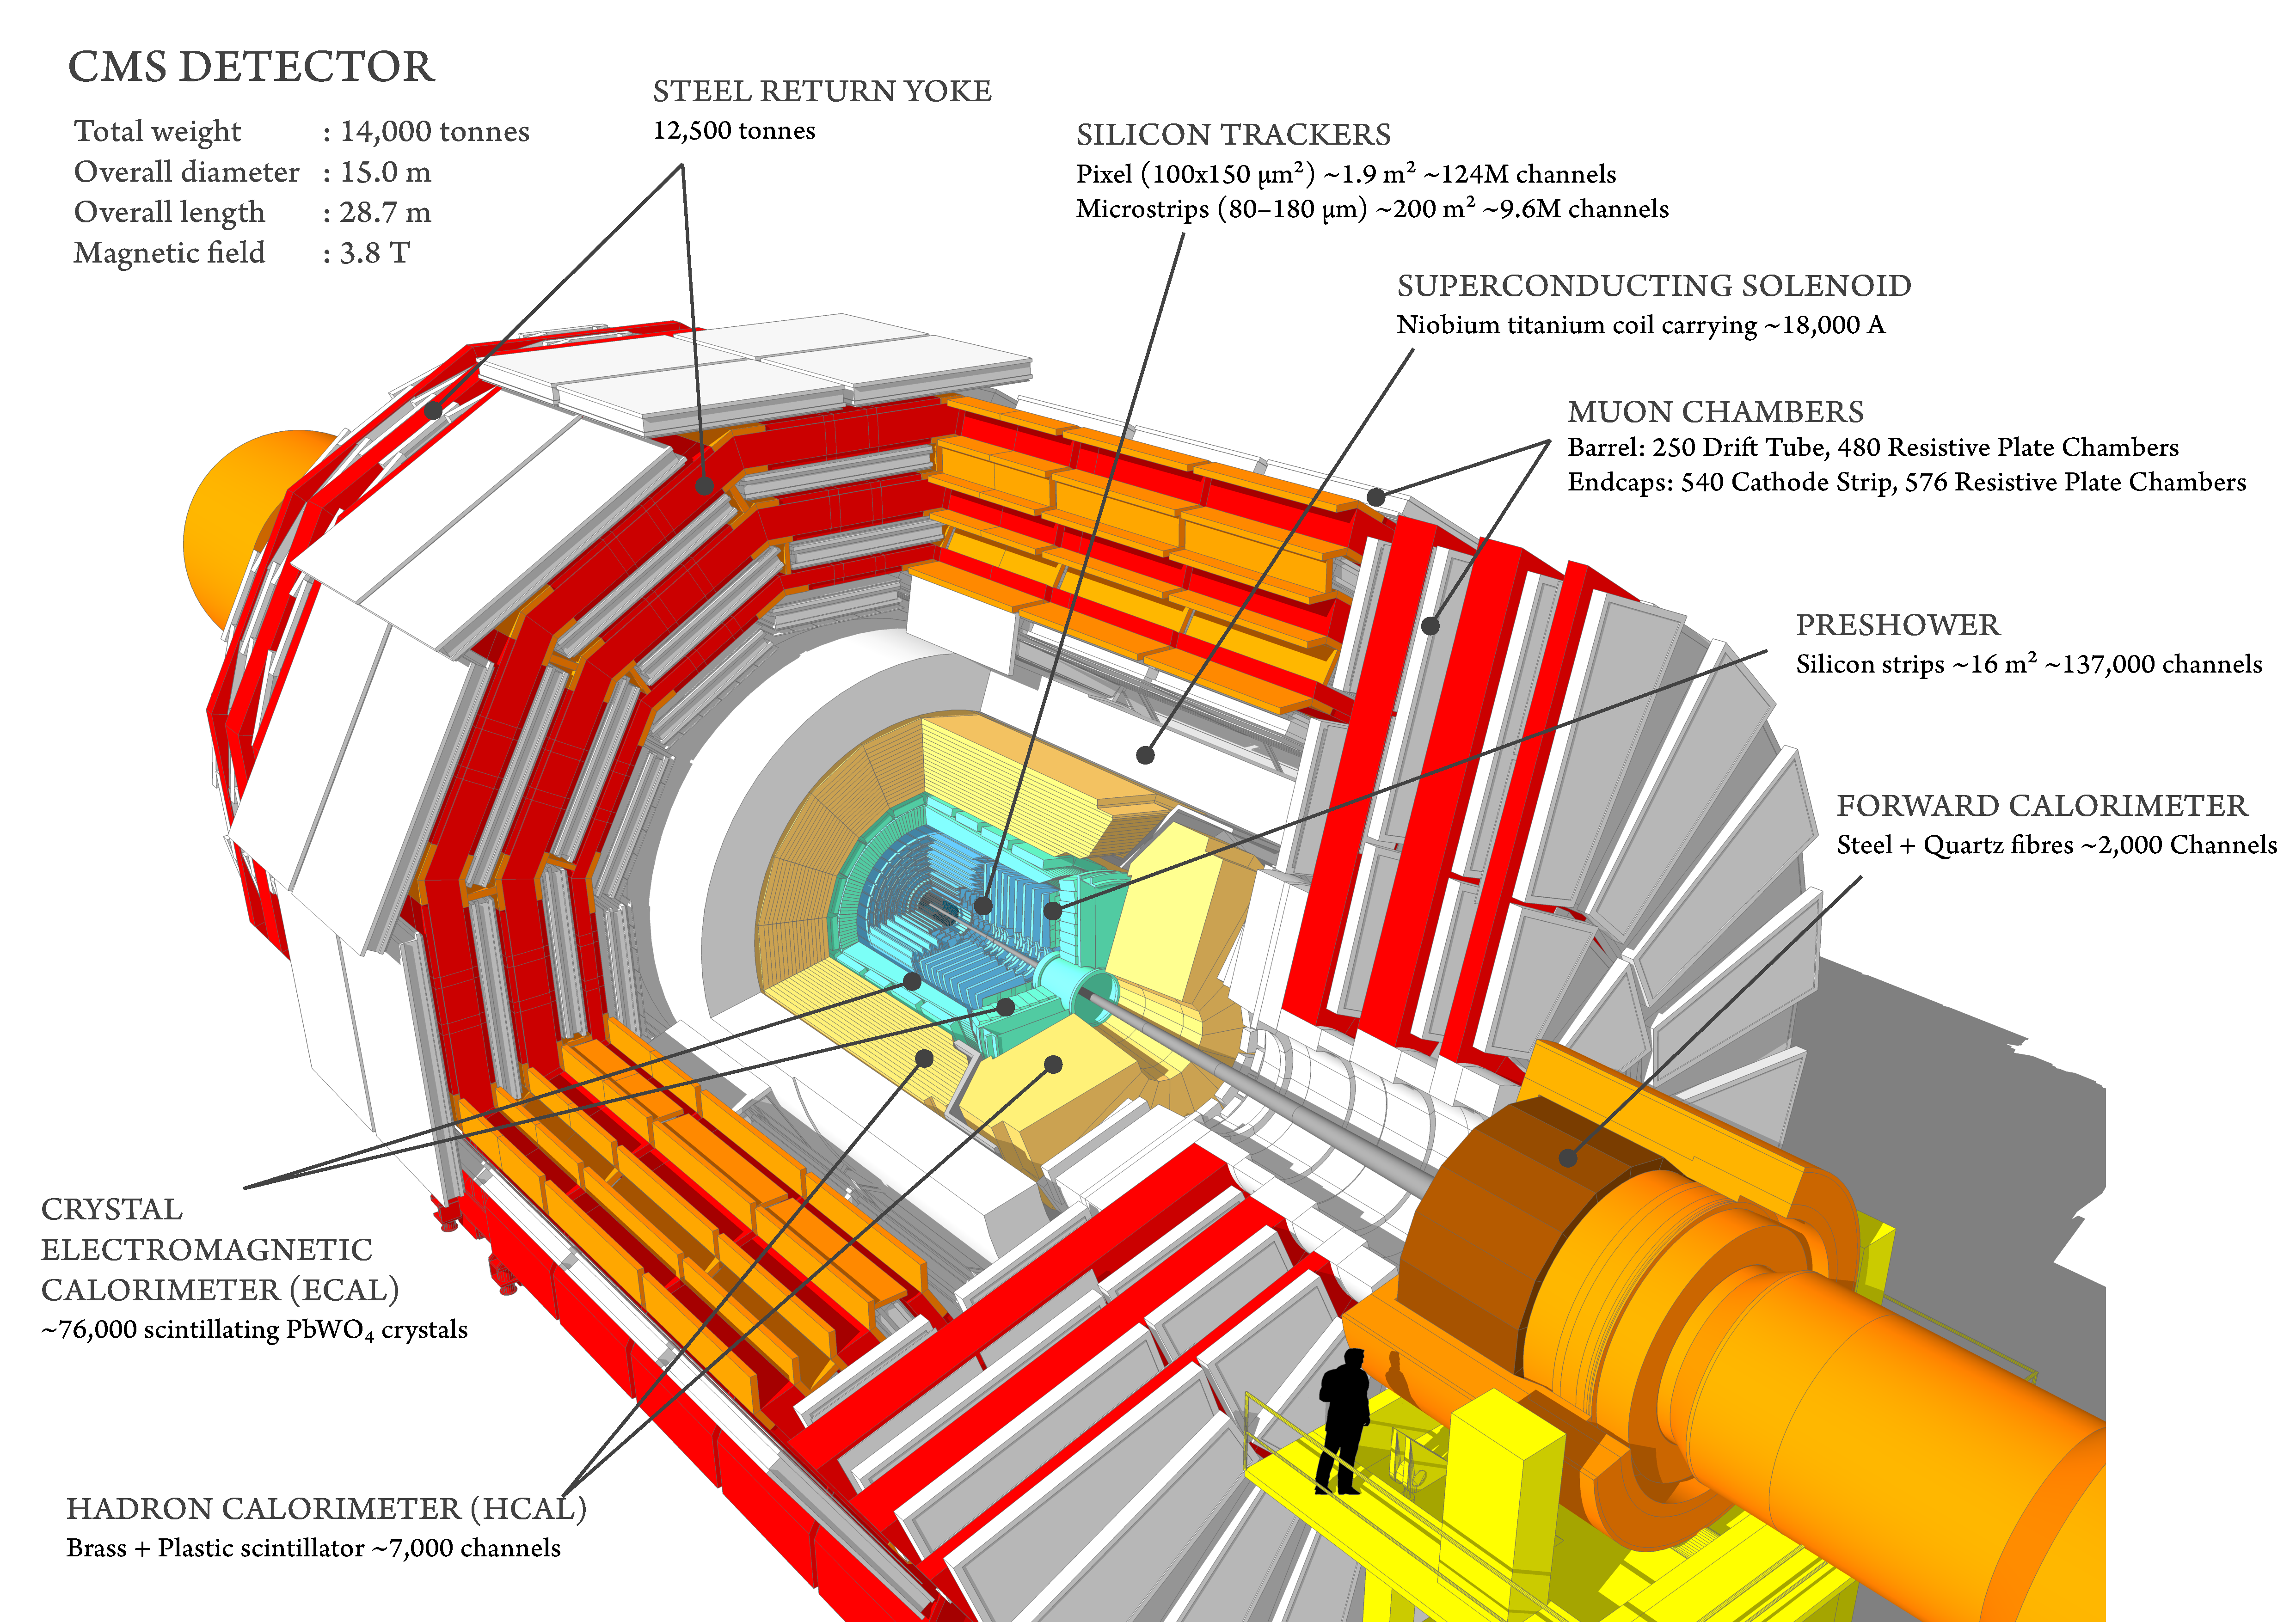
\includegraphics[width=15cm,height=15cm,keepaspectratio]{figures/cms/cms_cut_away.png}
    \caption{Cut out of the CMS detector showing its various subdetector components.} 
    \label{fig:cms_cut_out_view}
\end{figure}
%%%%%%%%%%%%%%%%%%%%
A few example particles and their associated tracks are shown in Fig.~\ref{fig:cms_particle_trajectories}.

Before discussing each subdetector in the following sections, it is useful to define the coordinate system used in CMS:
a typical, right-handed, three-dimensional Cartesian coordinate system $(x, y, z)$ is used, whose center $(0, 0, 0)$ is placed at the nominal \pp collision point within CMS.
The $x$-axis points towards the center of the LHC, the $y$-axis points vertically upward, and the $z$-axis points westward towards the Jura mountains, tangential to the beam direction.
Since CMS covers almost the entire spherical $4\pi$ steradians around the interaction point, it is convenient to use spherical coordinates $(r, \phi, \theta)$,
in which $r$ measures the radial distance in the $x$-$y$ plane, $\phi$ measures the azimuthal angle in the $x$-$y$ plane as measured from the $x$-axis, and $\theta$ measures the polar angle as measured from the $z$-axis.
When dealing with ultra-relativistic particles like those produced at the LHC, special relativistic effects like length contraction must be taken into account and so the coordinate $\theta$ becomes frame-dependent.
It is thus helpful to convert $\theta$ to the Lorentz-invariant quantity called pseudorapidity $(\eta)$,
defined as $\eta = -\ln [ \tan(\theta/2)]$. % Formula comes from: https://twiki.cern.ch/twiki/bin/view/Sandbox/GeorgeAlversonSandbox#Symbols_and_units_natural_units
% \begin{equation*}
%     \eta = -\ln \left(
%         \tan (\theta / 2)
%         \right)
% \end{equation*}
% which surround the 
%%%%%%%%%%%%%%%%%%%%
\begin{figure}[pbth]
\centering
\includegraphics[width=15cm,height=15cm,keepaspectratio]{figures/cms/cms_transverse_particletrajectories_corrected.png}
    \caption{
    A transverse view of CMS showing the ``filtration process'' as different particles pass through different subdetectors.
    A positron (solid red line) curves due to the presence of the magnetic field and gets stopped in the ECAL, creating an EM shower.
    A photon (blue dashed line) does not get detected at all by the Silicon Tracker, since it has no electric charge.
    It continues through to the ECAL and makes a shower here, like the positron.
    Charged hadrons (solid green line) will show curved tracks from the Silicon Tracker, may leave some trace in the ECAL, but primarily get stopped by the HCAL creating hadronic showers.
    Neutral hadrons (dashed green line) do not interact with the tracker, and only undergo EM showers a little in the ECAL, but show most energy deposits in the HCAL.
    Muons (solid blue line) are detected by the Silicon Tracker and then mostly pass through the other subdetectors without interacting until they finally reach the Muon System.
    % In fact you can even determine whether its charge is positive or negative since
    % q v cross B gives the direction of Force.
    % The velocity of the muon is out like this, and the B field is into the screen, so the applied force would be up like this for a positive particle. 
    Using the Lorentz force law and knowing which direction the magnetic field is pointing, one can deduce the sign of the charge of the particle. 
    Based on the radius of curvature from the trajectory, one can then calculate the momentum and energy of the particle.
    % We see that it's not curving up, but curving the other way so we know it must be negative.
    % Notice that since it is curving the opposite way from the muon so we know this is a positive particle.
    % Next up the solid green trajectory represents a charged hadron, like for example maybe an antiproton that got produced.
    % Notice that it would be the same sign as the muon because they curve in the same direction.
    } 
    \label{fig:cms_particle_trajectories}
\end{figure}
%%%%%%%%%%%%%%%%%%%%
% After the protons collide, they make a mess of all sorts of particles:
% electrons, lambda baryons, kaons, muons, photons...
% \section{The Silicon Tracker}\label{sec:tracker}

%%%%%%%%%%%%%%%%%%%%%%%%%%%%%
%----- Silicon Tracker -----%
%%%%%%%%%%%%%%%%%%%%%%%%%%%%%
\section{Silicon Tracker}
CMS is home to one of the world's largest silicon detectors, the so-called {\bf Silicon Tracker}.
The main purpose of the Tracker is to, well... \emph{track} the trajectories very precisely of outgoing particles from the IP.
It consists of two types of pure silicon detectors: the pixel detector and the strip detector, each of which is described next: 
% , and are absolutely necessary to \emph{track} the decay products from $pp$ collisions.

{\bf Pixel Detector:} The inner part, the closest subdetector of CMS to the IP, is the pixel detector made of minuscule silicon ``pixels'', as shown in Fig.~\ref{fig:tracker_real} (Left, pink).
Each pixel is 100$\mu$m x 150$\mu$m in size and, with 66 million of them, they altogether cover a sensitive area of 1.9 m$^2$. 
The pixel detector has the highest particle flux out of any other subdetector, since it sits only 8 cm away from the beam pipe:
it receives around 10 million particles per cm$^2$ per second.
The pixel detector is made of three cylindrical layers and two endcaps that surround the beam pipe.
Impressively, the pixel detector has around 6,000 connections (channels) per cm$^2$.

{\bf Strip Detector:} The second and outer part of the Silicon Tracker is called the strip detector, which has 10 million detector strips spread across 10 cylindrical layers.
The first 4 layers belong to the tracker inner barrel (TIB) and the remaining 6 layers belong to the tracker outer barrel (TOB), Fig.~\ref{fig:tracker_real} (Left, green and blue, respectively). 
Both the TIB and TOB have two endcaps associated with them, the TID and TEC, respectively.
Accounting for all of its components, the strip detector is sensitive to 200 m$^2$.
Fig.~\ref{fig:tracker_xs} gives a clearly-labelled transverse illustration of the pixel and strip detectors.
% It functions similarly to the pixels in that 
% It also has has slightly worse resolution than the pixel detector.
% Both the pixel and strip trackers have barrel and endcap components for nearly hermetic coverage around the beam pipe.
%%%%%%%%%%%%%%%%%%%%
\begin{figure}[pbth]
\centering
\includegraphics[width=0.49\textwidth,height=10cm,keepaspectratio]{Figures/silicon_tracker_simulated.png}
\includegraphics[width=0.49\textwidth,height=10cm,keepaspectratio]{Figures/silicon_tracker_real.jpg}
    \caption{
    (Left) A simulation of the Silicon Tracker, showing the 3 cylindrical layers of the pixel detector (pink), 4 layers of the TIB (green) and the 6 layers of the TOB (blue) of the strip detector.
    The endcap components are also shown.
    (Right) A real picture of the Silicon Tracker. Purdy, isn't it?} 
    \label{fig:tracker_real}
\end{figure}
%%%%%%%%%%%%%%%%%%%%
\begin{figure}[pbth]
\centering
\includegraphics[width=10cm,height=10cm,keepaspectratio]{Figures/silicon_tracker_transverse_view.png}
    \caption{A transverse view of the silicon pixel and strip detectors, explicitly labelling the different layers involved.}
    \label{fig:tracker_xs}
\end{figure}
%%%%%%%%%%%%%%%%%%%%

Consider the life of a particle produced from a $pp$ collision:
Starting at the IP, the produced particles first have an opportunity to interact with the Tracker (Fig.~\ref{fig:tracker_real}, Right).
Only charged particles will generate ``hits'' in the Silicon Tracker.
Therefore, photons, neutrons, and neutral pions, \eg, are invisible to the tracker.
Given enough hits and using sophisticated reconstruction software, we can determine precisely how the particle passed through the tracker.
It's essentially a fancy game of ``connect-the-dots'' to determine the particle's trajectory.
Figuring out the trajectory allows one to measure the radius of curvature, and therefore the momentum of the particle.
This is what makes the Silicon Tracker such an important subdetector.

Another major benefit of the Silicon Tracker is its assistance in vertex identification.
During pile up (multiple proton collisions happening within the same BX),
the tracker can distinguish between proton collisions with a resolution of about 
100 $\mu$m longitudinally and 50 $\mu$m transverse to the beam pipe.
This is crucial to being able to figure out which outgoing particles came from which $pp$ vertex.
Since the tracker wasn't built to catch particles, they usually continue on to the next subsystems.
Thus, CMS must be built as a kind of ``particle filter''.
Electrons and photons are the first to be filtered out by the Electromagnetic Calorimeter...

\subsection{The Pixel Detector}\label{subsec:pixel}

\subsection{The Strip Detector}\label{subsec:strip}
% \section{The Calorimeters}
\label{sec:calo}

\subsection{Electromagnetic Calorimeter}

Particles that survive the Tracker will then encounter the Electromagnetic Calorimeter (ECAL).
The ECAL is a hermetic homogeneous sub-detector consisting of a barrel part (EB) and two endcap parts (EE).
The EB contains 61200 lead tungstate (PbWO$_4$) crystals while each EE contains 7324 crystals.
Due to its short radiation length (0.89 cm) and high density (8.28 g/cm$^3$),
PbWO$_4$ is a good material to use in the ECAL.
Conveniently after 1 bunch crossing (25 ns), nearly 80\% of the scintillated light is emitted.

\begin{figure*}[!htb]
    \centering
    \captionsetup{justification=justified}
    \includegraphics[width=0.95\textwidth]{figures/ECAL/xs_whiteblack.jpeg}
    \caption{Cross sectional view of the electromagnetic calorimeter of CMS.
             Figure taken from Ref.~\cite{jinst:cms_exp}.}
    \label{fig:ecal_xs}
\end{figure*}

whose purpose is to absorb photons and electrons and detect their energies and directions.

%%%%%%%%%%%%%%%%%%
%----- ECAL -----%
%%%%%%%%%%%%%%%%%%
After particles pass through the Silicon Tracker system, they encounter the {\bf Electromagnetic Calorimeter} (ECAL). 
This is a scintillating subdetector made out of approximately 78,000 beautiful, transparent, and heavy ${\rm PbWO_{4}}$ crystals, as shown in Fig.~\ref{fig:ecal_crystals} (Left).
Each crystal weighs 1.5 Kg but has only the volume of a small cup of coffee. 

%%%%%%%%%%%%%%%%%%%%
\begin{figure}[pbth]
\centering
\includegraphics[width=0.49\textwidth,height=10cm,keepaspectratio]{Figures/ECAL_crystals_fancy_lab.jpg}
\includegraphics[width=0.49\textwidth,height=10cm,keepaspectratio]{Figures/ECAL_crystal_sizecomparison.jpg}
    \caption{
    (Left) ECAL crystals are grown in a lab.
    (Right) Although made mostly of metal, ECAL crystals are transparent and have a photomultiplier detector attached at the end.} 
    \label{fig:ecal_crystals}
\end{figure}
%%%%%%%%%%%%%%%%%%%%
Electrons and photons interact electromagnetically with the ECAL, creating an electromagnetic (EM) shower, and effectively get trapped here.
The ECAL crystals then give off light (\emph{scintillate}) in proportion to the amount of energy deposited by the electron or photon. 
The scintillator photons are detected by a photomultiplier detector attached to the back of each ECAL crystal (Fig.~\ref{fig:ecal_crystals}, Right).
The ECAL has a barrel component and endcap components.

How does one distinguish between an electron energy deposit in the ECAL system versus and a photon deposit?
The electron will leave hits in the Tracker whereas a photon is electrically neutral and will not generate any signal in the Silicon Tracker. 
So long as the Tracker and ECAL communicate effectively with each other, then they help distinguish between electrons and photons.
Charged hadrons also interact with the ECAL, but only minimally. They very often punch through the ECAL system.
Neutral hadrons can be detected by the ECAL preshower near the ECAL endcaps. 
which helps distinguish a single photon from $\pi^{0}$ mesons as they decay into two photons with a narrow opening angle, making it look as if the two photons are a single photon.

What about those hadrons? They got through the ECAL... To detect hadrons effectively, we need a Hadron Calorimeter.
% That's what we see here with the blue dashed line (the photon) and the red line (the positron).

%%%%%%%%%%%%%%%%%%
%----- HCAL -----%
%%%%%%%%%%%%%%%%%%
\subsection{Hadron Calorimeter}
By the time particles reach the {\bf Hadron Calorimeter} (HCAL), the only kind which remain (usually) are muons and hadrons.
At 1 meter thick, the HCAL is a brass scintillator and its primary purpose is to catch and record the energies of hadrons.
Similar to the ECAL, the HCAL will scintillate in proportion to the amount of energy of the captured particle. 
The incoming hadrons will \emph{hadronize} (\ie, produce a hadronic shower), generating jets of quarks and gluons which are bound in various ways forming protons, neutrons, pions, kaons, \etc.
Interestingly, the HCAL is made using over a million old, brass shell casings from the Russian Navy back from World War II.
% kinds of particles which have not decayed on their own or were not caught by the ECAL, ,  or when it catches hadronic material: stuff made of quarks, like . 


% \section{The Solenoid and the Steel Return Yoke}
\label{sec:solenoid}

The Compact Muon \emph{Solenoid} sports one of the world's most energetic solenoids and is paramount to the success of CMS.
Particles that exit the HCAL~\ref{subsec:hcal} arrive at the cylindrical magnet which is 12.5 \meter in length, has a bore diameter of 6.3 \meter when cold, and generates a uniform 3.8 \tesla magnetic field parallel to the beam line.
To generate such a large and uniform magnetic field, a current of 18,000 A travels through superconducting Nb-Ti coils inside the approximately 360 \meter$^3$ volume (Fig.~\ref{fig:cms_magnetic_field}).
This magnetic field is 100,000 times stronger than that of Earth's, as measured at the surface, and stores a massive 2.6 GJ of energy - approximately equivalent to the kinetic energy of an Airbus A320 in flight.
%%%%%%%%%%%%%%%%%%%%
\begin{figure}[pbth]
    \centering
    \includegraphics[width=15cm,height=15cm,keepaspectratio]{figures/cms/solenoid/CMS_longitudinal_view_magnetic_field.png}
        \caption{
        A longitudinal cross section of CMS showing the values of the magnetic field over the volume of CMS and various field lines. 
        The magnetic field reaches its maximum of 3.8 T in the center of the detector.}
        \label{fig:cms_magnetic_field}
    \end{figure}
    %%%%%%%%%%%%%%%%%%%%

% the direction in which the protons collide, which we call the z direction.
When charged particles travel through a magnetic field, a Lorentz force is applied to them, thereby separating out the particle tracks as they travel away from the interaction point.
The large magnetic field generated by CMS assists in The relative change in momentum (\ie the momentum resolution) is 
% As the charged particles bend out and away from the beam pipe, they pass through the silicon tracking system, which has excellent resolution ""
% Imagine CMS as a giant camera that takes a picture every few ns of the outgoing particles. 

\textbf{Steel Return Yoke:} 
Most of the mass of CMS comes from the \emph{steel return yoke} which helps to redirect the magnetic field back on itself. 
The yoke system constitutes 10,000 tonnes, which is 89\% of the total mass of CMS.
It is comprised of 5 wheels and 2 endcaps

% \section{The Muon System}
\label{sec:muon_sys}
Although it is the farthest system from the interaction point, the muon system is one of the most important subsystems within the Compact \emph{Muon} Solenoid experiment.
%  is the {\bf Muon System} and is what puts the {\it Muon} in Compact {\it Muon} Solenoid.
Of the particles emerging from the interaction point, electrons and photons are absorbed by the ECAL (Sec.~\ref{sec:ecal}) and hadronic matter is absorbed by the HCAL (Sec.~\ref{sec:hcal}).
This filtration process leaves only neutrinos and muons to enter the muon system, which is the outermost detector situated past the solenoid (Sec.~\ref{sec:solenoid}).
As mentioned in Ch.~\ref{ch:theory}, neutrinos are the only weakly interacting, electrically neutral SM particles which makes them incredibly difficult to detect directly.
In fact, neutrinos interact with normal matter so little that a light-year of lead (9.46 \emph{trillion}\Km) would only stop half of the neutrinos moving through it.
So, detection of neutrinos produced from \pp collisions is inferred via \MET on a per-event basis.
Muons, on the other hand, have a mass of 105.7\MeV (relatively heavy for a weakly-interacting, electrically-charged particle) and live approximately \tentothe{17} times longer than a Higgs boson: the average lifetime of a muon is $\tau_{\Pmu} = 2.2 \times \tentotheminus{6}\snd$.
% which interestingly will travel way outside of CMS before decaying, upwards of 100s of kilometers before decaying to an electron and neutrino (neutrinos are the only particles which CMS can't explicitly detect).
These properties are what determined the properties of the muon system within CMS to consist of its four main subdetectors, each of which is described in the following subsections:
\begin{enumerate}
    \item CSC (cathode strip chambers, Sec.~\ref{sec:csc}),
    \item DT (drift tubes, Sec.~\ref{sec:dt}),
    \item RPC (resistive plate chambers, Sec.~\ref{sec:rpc}),
    \item GEM (gas electron multiplier, Sec.~\ref{sec:gem}).
\end{enumerate}

\subsection{Cathode Strip Chambers}
\label{sec:csc} 

\textit{\textbf{Overview:}}
A cathode strip chamber (CSC) is a multi-wire proportional chamber capable of precisely measuring the position of muons which enter and ionize the gas within.
Spatial coordinates are obtained by the collection of electrical signals along the cathode strips $(\phi)$, anode wires $(r)$, and across multiple CSC layers $(z)$.
CSCs are found exclusively on the two endcaps of CMS---with each endcap bearing 270 chambers (Fig.~\ref{fig:cms_endcap})---so that there are 540 CSCs in total.
The chambers are arranged azimuthally around the beam pipe in four disks per endcap allowing for contiguous coverage in $\phi$.
In total, the CSC system provides an effective detection area of about 5000$\meter^2$, has a total gas volume that exceeds $> 50\meter^{3}$, and contains over 400\,000 read-out channels.
%%%%%%%%%%%%%%%%%%%%
\begin{multiFigure}
    \centering
        \addFigure{0.44}{figures/cms/muonsys/csc_endcap_cutaway.png}
        \addFigure{0.52}{figures/cms/muonsys/csc_endcap_real.png}
    \captionof{figure}
        [Cathode strip chambers line the disks of CMS]
        {Cathode strip chambers line the disks of CMS.
        \;A) Simulated cut-out view of the ME$+$ endcap, with the coordinate system of CMS on the left-hand side.
        Human for scale.
        \;B) The actual ME$-$2 disk of CMS is shown, revealing its ME$-$2/1 and ME$-$2/2 rings of CSCs.
        Figures taken from~\cite{collaboration_cms_2008}.}
    \label{fig:cms_endcap}
\end{multiFigure}
%%%%%%%%%%%%%%%%%%%%
% Longitudinal cross section
\begin{multiFigure}
    \centering
        \includegraphics[width=15cm,height=10cm,keepaspectratio]{figures/cms/cms_longitudinal_view.png}
    \captionof{figure}
        [Longitudinal cross section of CMS with pseudorapidity values shown]
        {Longitudinal cross section of CMS showing the different pseudorapidity values ($\eta$), along with the different subdetector regions.
        Figure taken from~\cite{cms_long_xs_view}.}
    \label{fig:cms_long_view_subdetectors}
\end{multiFigure}
%%%%%%%%%%%%%%%%%%%%
\textit{\textbf{Design:}}
Each CSC is trapezoidal in shape with its narrow end pointed toward the beam pipe (Fig.~\ref{fig:csc_guts}).
The chambers are arranged in rings and each chamber subtends either 10\degrees or 20\degrees in $\phi$, as described in Sec.~\ref{sec:csc_numbering}.
The CSCs cover the pseudorapidity range of $0.9 < \abseta < 2.4$ (Fig.~\ref{fig:cms_long_view_subdetectors}).

A single CSC is composed of six layers (or \emph{gas gaps}), each of which is filled with a carefully prepared gaseous mixture\footnote{
    The gas mixture ratio of Ar:CO$_{2}$:CF$_{4}$ was chosen to be 5:4:1 to maximize the lifetime of the CSCs as they endure radiation damage through years of use.
    The CO$_{2}$ is used as a non-flammable quencher to reach even larger electron multiplicities, while the CF$_{4}$ helps prevent polymerization along (aging of) the wires.
    }
of Ar:CO$_{2}$:CF$_{4}$ (Fig.~\ref{fig:csc_separatelayers}).
Within every layer, the gas mixture surrounds approximately 80 copper strips, each of which spans radially away from the interaction point.
A single strip is about 8.4\mm wide at the narrower end of the CSC, about 16\mm at the wider end, and is separated from its neighboring strip by about 0.5\mm.
Per layer, the inner gas also surrounds over 1000 gold-plated tungsten wires, which are oriented azimuthally (so approximately orthogonal to the strips).
% (except in the CSCs closest to the interaction point)
Each wire is approximately 50\mum in diameter and separated from its neighboring wire by about 3.2\mm.
A collection of 16 consecutive wires forms a \emph{wire group}, which is about 5\cm wide and creates a single anode read-out channel.
A single wire plane has five independently controlled HV segments (Fig.~\ref{fig:csc_guts}).
The largest CSCs are 3.4\meter long as measured along a strip and 1.5\meter wide as measured along a wire.
% CSC separated layers.
%%%%%%%%%%%%%%%%%%%%
\begin{multiFigure}
    \centering
        \includegraphics[width=0.9\textwidth,keepaspectratio]{figures/cms/muonsys/csc_separatedlayers.jpeg}
    \captionof{figure}
        [Cross section of CSC revealing the gas gaps]
        {Exploded view of the cross section of a CSC showing how the 7 panels come together to form the 6 gas gaps between the panels.
        Figure taken from~\cite{collaboration_cms_2008}.}
    \label{fig:csc_separatelayers}
\end{multiFigure}
% CSC guts.
%%%%%%%%%%%%%%%%%%%%
\begin{multiFigure}
    \centering
        \addFigure{0.41}{figures/cms/muonsys/csc_cutaway_view_new.png}
        \addFigure{0.55}{figures/cms/muonsys/csc_stripsandwires.png}
    \captionof{figure}
        [Views of an exposed CSC showing the wires and strips inside]
        {Views of an exposed CSC showing the wires and strips inside.
        \;A) CSC with its top layer exposed.
        Thin, horizontal, gold-plated tungsten wires span the entire width of the CSC. 
        Thicker, vertical strips run along the length.
        \;B) More detail inside a CSC showing the radial strips, horizontal wires, and 5 segments separating the wires.
        Figures taken from~\cite{collaboration_cms_2008}.}
    \label{fig:csc_guts}
\end{multiFigure}
% In conjunction with the Silicon Tracker measurements, muon momentum can be measured to a precision of 
% {\bf Quick Mention:} The University of Florida has been one of the main contributors to the CSC system and was home to one of the testing and assembly facilities before shipping the CSCs off to CERN.

\textit{\textbf{Physics:}}
As a muon passes through a CSC layer, it has the opportunity to interact with and ionize an Ar atom in the gas mixture.
The wires are under high voltage (3600\,V) which causes the ionized electron to accelerate towards the positively charged strips.
The accelerating electron collides with and ionizes Ar atoms along its path toward the strip.
This liberates even more electrons, thus forming an \emph{electron avalanche} (Fig.~\ref{fig:elec_avalanche}).
The total number of ionized electrons per initial electron is referred to as the \emph{multiplicity} (or \emph{gas gain}), which can reach as high as 100\,000.
% Electron avalanche.
%%%%%%%%%%%%%%%%%%%%
\begin{multiFigure}
    \centering
        \includegraphics[width=15cm,height=10cm,keepaspectratio]{figures/cms/muonsys/csc_elec_avalanche_old.png}
    \captionof{figure}
        [Muon traverses a CSC, ionizing the gas within and creating an electron avalanche]
        {A muon passes through one of the gaseous layers of the CSC, ionizing the gas mixture and inducing a charge on the anode wires and cathode strips.
        Figure taken from~\cite{collaboration_cms_2008}.}
    \label{fig:elec_avalanche}
\end{multiFigure}
%%%%%%%%%%%%%%%%%%%%

The electron avalanche is collected by a cathode strip and becomes an electrical signal.
This signal is processed by the cathode front-end boards (CFEBs).
The Ar$^+$ ions similarly distribute a charge signal onto the negative wires.
The cluster of charge that arrives at a strip is more widely spread than the charge which arrives along a wire.
Therefore, comparator logic is implemented on the strips to narrow down the precision to the order of 100\mum by using half-strip information (Fig.~\ref{fig:comparators}).
% Comparators and strips.
%%%%%%%%%%%%%%%%%%%%
\begin{multiFigure}
    \centering
        \addFigure{0.49}{figures/cms/muonsys/csc_comparator_logic.png}
        \addFigure{0.49}{figures/cms/muonsys/csc_comparator_logic_muontraverse.png}
    \captionof{figure}
        [Comparator logic as a muon traverses the layers of a CSC]
        {Comparator logic as a muon traverses the layers of a CSC.
        \;A) Comparators are used to compare neighboring strip cluster charge to determine on which half-strip the peak charge resided.
        \;B) Muon passes through all six layers of a CSC inducing charge on various half-strips.
        Figures taken from~\cite{collaboration_cms_2008}.}
    \label{fig:comparators}
\end{multiFigure}
%%%%%%%%%%%%%%%%%%%%

The muon passes through the next 5 layers of the CSC, further ionizing the gas mixture and generating electrical signals along the wires and strips.
A signal on a wire provides an $r$-coordinate, on a strip provides a $\phi$-coordinate, and through the other layers provides a $z$-coordinate.
Taken together, this information helps to reconstruct the three-dimensional trajectory of the muon.
% The AFEBs then digitize this analog signal using ADCs and 

The number of hits recorded by the CSC will determine if an event was significant enough to be worth saving.
If so, then its precise positions on the wires and strips will be read out by the Data Acquisition (DAQ) system and be stored for further data analysis.
When a CSC is taking live data it can resolve approximately 2\mm in $r$-$\phi$, whereas during offline analysis the resolution improves by a factor of more than 20:
the ME1/1 and ME1/2 chambers can resolve distances as small as 75\mum in $r$-$\phi$, while the other chambers can resolve 150\mum.
It is worth noting that a CSC can accommodate up to 1$\KHz/\cmns^2$.

% Each CSC cost about \$100,000 to make, so very quickly this becomes an expensive project.

% Gas gap is 9.5~\mm.

% \subsection{Endcap Muon Electronics}
% In order to conclude that a muon definitely passed by the muon detectors, a very sophisticated electronics system has been developed. 

% Hmm... EMU is just for the endcaps. This system is called "EMU" and 

% Next I am going to elaborate more on the CSCs, since my first experience with CMS hands-on work with CSCs. 

% The muon barrel system, after it talks with the tracker system, has a muon pT resolution of 1.5% in the barrel and ~6% in the endcap.

% Trigger system:
% Since the event  rate and data rate are so high, and most of the events are uninteresting, typical physics,
% we need a fast-working filtration system to sift through the good and bad events. 
% We want to "trigger" on the good events but only have about 4 μs to do so. 
% This is the job of the L1 trigger and and the High-Level Trigger. 

\subsubsection{CSC Numbering Scheme}
\label{sec:csc_numbering}
The two endcaps are labelled as `ME$+$' and `ME$-$', depending on whether they are situated in the $+z$ direction or $-z$.
Both endcaps are structurally symmetric, so it is sufficient to discuss only one in detail.
The ME$+$ endcap has four disks: ME$+$1 is the first disk and the one closest to the interaction point, while ME$+$4 is the fourth and the farthest away. 
Within each disk, there are either two or three \emph{rings} of CSCs, as shown in Fig.~\ref{fig:cms_long_view_subdetectors} (green).
These rings are labelled as ME$+D$/$R$, where $D$ indicates the disk number and $R$ indicates the ring number.
For example, ME$+$2/1 refers to the second disk and the first ring (the ring closest to the beam pipe).
All rings contain 36 CSCs, except for ME$\pm X$/1, for $X= 2,3,4$, which contain only 18 CSCs.
Finally, the CSCs are given one final number to label them on the ring:
the CSC that sits along the positive $x$ axis in the coordinate system of CMS is given the number `01', \eg ME$+$4/2/01. 
The CSCs are then numbered incrementally following the positive azimuthal direction.

\subsection{Drift-Tube Chambers}
\label{sec:dt}

\textbf{\textit{Overview:}}
Functionally similar to but structurally different from a CSC (Sec.~\ref{sec:csc}), a DT is a collection of gaseous detector cells (Fig.~\ref{fig:dt_superlayers}).
A single DT cell has an anode wire and two cathode strips and operates on the same principle as a CSC, providing timing and position measurements of muons (Fig.~\ref{fig:dt_cell}).
While CSCs are found only on the endcaps of CMS, drift-tube chambers (DTs) are placed exclusively along the barrel (Fig.~\ref{fig:dt_locations}).
The DT system is therefore composed of concentric cylindrical stations, with the central axis parallel to the beam pipe.
Altogether, there are 250 DTs built inside of, between, and outside of the iron yoke.
% DT Chamber.
%%%%%%%%%%%%%%%%%%%%
\begin{multiFigure}
    \centering
        \includegraphics[height=9cm,keepaspectratio]{figures/cms/muonsys/drifttube_superlayers.jpeg}
    \captionof{figure}
        [Cross section of an entire drift tube chamber]
        {Cross section of an entire drift tube (DT) chamber showing 3 superlayers (SLs) and the interior honeycomb plate.
        Two SLs are indicated by the blue rectangles, whose cells (orange rectangle) have anode wires (red dots) oriented parallel to the beam pipe.
        The third SL is indicated by the green rectangle and is placed orthogonally to the other two SLs.
        Figure taken from~\cite{collaboration_cms_2008} and modified with orange, green, and blue rectangles and red dots.}
    \label{fig:dt_superlayers}
\end{multiFigure}
% DT Cell.
%%%%%%%%%%%%%%%%%%%%
\begin{multiFigure}
    \centering
        \includegraphics[height=5.5cm,keepaspectratio]{figures/cms/muonsys/drifttube_xs.jpeg}
    \captionof{figure}
        [Cross section of a single drift tube cell]
        {Cross section of a single drift tube cell showing the drift lines (light blue), isochrone lines (dark blue), dimensions of the cell, and locations of the anode wire and cathode strips.
        Figure taken from~\cite{collaboration_cms_2008}.}
    \label{fig:dt_cell}
\end{multiFigure}
%%%%%%%%%%%%%%%%%%%%
% DT locations.
\begin{multiFigure}
    \centering
        \includegraphics[width=15cm,height=10cm,keepaspectratio]{figures/cms/muonsys/drifttube_locations.jpeg}
    \captionof{figure}
        [Cross section of the CMS barrel showing the locations of the drift tubes]
        {Cross section of the CMS barrel showing the locations and the numbering scheme of the drift tubes in the barrel.
        Figure taken from~\cite{collaboration_cms_2008}.}
    \label{fig:dt_locations}
\end{multiFigure}
%%%%%%%%%%%%%%%%%%%%

\textbf{\textit{Design:}}
The first three stations contain 60 DTs each, while the station farthest from the beam pipe contains 70 DTs.
The DTs are distributed among 5 wheels, 4 stations, and 12 sectors within the muon barrel (MB) system which uses the following numbering scheme:
MB/$W$/$A$/$S$,
where $W$ is the wheel number ($-$2 to 2),
$A$ is the station number (1 to 4),
and $S$ is the sector number (1 to 12).
This accounts for only $5 \times 4 \times 12 = 240$ chambers, so the remaining 10 DTs are found in station 4, sectors 4 and 10, in each wheel (Fig.~\ref{fig:dt_locations}).

Each tube cross section is $13 \times 42\mm^{2}$, within which a single anode wire is made of gold-plated stainless-steel that has a diameter of 50\mum.
Different voltages are applied to the anode wires ($+$3600\,V), electrode strips ($+$1800\,V), and cathode strips ($-$1200\,V).
The gas mixture within a DT is similar to that of a CSC, containing approximately 85\% Ar $+$ 15\% CO$_{2}$.

\textbf{\textit{Physics:}}
DTs are a good choice for the barrel because of the low rate and low strength of magnetic field.
They offer a uniform drift field of 1.5\,KV/cm.
A high \pt muon track will cross all 4 DT stations within the pseudorapidity range of $\abseta < 0.8$.
The reconstruction efficiency of such a track is better than 95\%.

A single SL has a time resolution of only a few nanoseconds which provides excellent bunch crossing identification.
To assist in determining muon \pt and timing, the DT system delivers the following muon track segment information to the L1 trigger:
the position of the center of gravity (to a precision of 1.5\mm) and the corresponding angle (to a precision of 20\,mrad), with respect to the SL reference frame.
The total resolution of a DT in the $r$-$\phi$ plane is about 100\mum which is comparable to the deviation caused by multiple scattering, for a muon with $\pt \le 200\GeV$.

The gas gain is comparable to that of a CSC (about 100\,000).
The maximum drift distance in a DT is 21\mm, as can be seen in Fig.~\ref{fig:dt_cell}, which corresponds to a drift time of 380~\ns.

\subsection{Resistive Plate Chambers}
\label{sec:rpc}

\textbf{\textit{Overview:}}
Even though CSCs (Sec.~\ref{sec:csc}) and (Sec.DTs~\ref{sec:dt}) cover the entire pseudorapidity range of $0 < \abseta < 2.4$, redundancy is important.
Therefore, resistive plate chambers (RPCs) are placed in both the barrel and endcaps to provide excellent timing and spatial resolution---comparable to that of scintillators---to supplement the measurements of the CSC and DT systems.
RPCs are fast, gaseous detectors that serve as a muon trigger system.
Muons traversing through the RPCs ionize the gas and cause an avalanche, which is measured by the plate.

\textbf{\textit{Design:}}
% RPCs consist of two highly-resistive parallel plates (bakelite electrodes), one positively-charged and the other negatively-charged, separated by a 2-\mmns gap of gaseous volume.
The gas is a three-component mixture composed of 95.2\% C$_2$H$_2$F$_4$, 4.5\% $i$C$_4$HO (isobutane), and 0.4\% SF$_6$ with a 35--40\% humidity, and kept at 21$\degrees$C.
The RPC system consists of 480 rectangular chambers found in the barrel and are oriented parallel to the beam pipe, each at 2.455\meter long.
There are also 288 RPCs found on each endcap.
RPCs have better time resolution compared to the 25\ns between two consecutive \pp bunch crossings. 

% Gas mixture comprised of 96.2\% C$_{2}$H$_{2}$F$_{4}$ (1,1,1,2-tetrafluoroethane) $+$ 3.5\% $i$C$_{4}$H$_10$ (isobutane) $+$ 

\textbf{\textit{Physics:}}
Muons passing through RPC chambers ionize the gas, causing an avalanche of electrons.
The electrodes are transparent to the signal, which are instead picked up by the external metallic strips after a small but precise time delay.
The pattern of strips which are hit gives a rapid measure of the muon's momentum, which is then used by the trigger to make an immediate decisiosn about whether the data are worth keeping.
RPCs combine a good spatial resolution with an excellent time resolution of just one nanosecond. 

\subsection{Gas Electron Multipliers}
\label{sec:gem}

\textbf{\textit{Overview:}}
Gas Electron Multipliers (GEM) are a new addition to the CMS muon system and will complement existing detectors in the forward regions close to the beampipe where radiation levels and event rates will significantly increase during Phase-2 of the LHC.
GEM systems in the endcaps will improve the measurement of the polar muon bending angle, allowing the muon trigger to cope with higher rates.
The GEMs will further extend the muon system coverage in the far-forward regions. 

\textbf{\textit{Design:}}
GEMs are gaseous detectors featuring a GEM foil, which consists of a 50-\mumns-thick insulating polymer (polyimide) encased on top and bottom by copper conductors.
Microscopic holes are etched in a regular hexagonal pattern throughout the foil.
The GEM chambers consist of two PCBs containing the gas volume filled with an Ar/CO$_2$ gas mixture separated by a stack of three GEM foils.
The GEMs feature a large area of about 0.5$\meter^2$.
The first batch comprising 144 chambers was installed during Long Shutdown 2 on the first disk of the two endcaps.
These chambers will contribute to data-taking during Run 3 of the LHC.
Additionally, two more disks of GEM chambers will be installed in each endcap during 2024--2026, before the Phase-2 upgrade.

\textbf{\textit{Physics:}}
The chambers are filled with an Ar/CO$_2$ gas mixture, which is ionized by muons traversing the detector system.
This generates a potential difference across the foils, which generates sharp electric fields in the holes.
Electrons created during the ionization process drift towards the foil and are multiplied in the holes, resulting in an electron avalanche that induces a readout signal on finely-spaced strips.





% We can only assume that we produced neutrinos when momentum is apparently not conserved in an event. 
% When the protons collide at the IP they have nearly zero momentum perpendicular to the beam pipe. 
% This is called transverse momentum, because it's well... transverse to the beam pipe, the z direction.
% If we track, tag, capture all the outgoing particles and reconstruct their transverse momenta, 
% if we find out that it is NOT zero by a large amount, then we say that 

% The main purpose of the Muon System is to precisely determine the position and timing of muons.
% \begin{enumerate}
%     \item 
%     % for offline analysis.
%     \item Generate muon trigger primitives for the Level-1 trigger system.
% \end{enumerate}
% Similar to the Silicon Tracker, the Muon System doesn't try to capture the muons passing through it;
% instead it just tracks their positions. 
% In fact our very own Andrey, Guenakh, and Darin have been instrumental in implementing CSCs. 
% There's also an assembly hall downstairs where CSCs were constructed and tested 
% The  specializes muons. Au contraire; it \textit{specializes} in muon detection. 
% The Compact \textit{Muon} Solenoid would be a pretty hypocritical name if CMS did not detect muons. Au contraire; it \textit{specializes} in muon detection. 
% P
%It would be an ironic name if it did not detect muons well. 

% This concludes the overall design and purpose of the subdetectors that make up CMS.
% Since I have had hands-on experience working on CSCs, I will discuss the CSC components and how it works in more detail in the subsection below.

% \section{Trigger System}
\label{sec:trigger}
% TODO: Add a trigger pic.
% TODO: Add more refs.
Collection of collision data by CMS for each and every interaction under nominal LHC conditions would require 40\TB/sec, which is an insurmountable task for the CERN computing farm, whose processing is limited by CPU performance and storage capacity.
Moreover, most proton collisions at the LHC arise from soft interactions and are highly unlikely to contain signatures of new physics, meaning they are of little interest.
Hence a trigger system is designed to reduce the event collection rate to 100\KHz by rejecting uninteresting events while keeping potentially interesting ones.
CMS implements a two-stage trigger system, the first of which is the Level-1 (L1) trigger, which filters events and passes them to the High-Level Trigger (HLT).

Triggers may be prescaled for two reasons:
firstly, different physics processes are characterized by different cross sections and,
secondly, the trigger must keep up with luminosity changes.
For the former, a prescale may be used to keep large inputs under control by, for example, recording only 1 out of every $x$ collisions, where $x$ is the prescale value.
This may be implemented if a process is far more likely to be recorded in order to reduce the rate.
For the latter, it is important to note that as the luminosity drops, prescales can be relaxed and can therefore change within the same fill.
A trigger can be prescaled at both levels in the CMS trigger system.

\subsection{The Level-1 Trigger}
\label{sec:L1_trig}
The Level-1 trigger reduces the event rate from 50\MHz to 100\KHz with a latency of 3.2\mus by utilizing Field Programmable Gate Arrays (FPGAs) and Application Specific Integrated Circuits (ASICs).
The L1 trigger uses only coarsely segmented data from the calorimeters and muon detectors while maintaining all of the high-resolution data in pipeline memories in the front-end electronics.
The L1 trigger features several algorithms (L1 bits or seeds) to store a general description of the event content from events that are accepted, which is then passed to the HLT for further event processing.

\subsection{The High-Level Trigger}
\label{sec:hlt}
The HLT is a software system organized into a set of algorithms known as ``paths'' designed to select specific event topologies, thus reducing the output rate from 100\KHz to approximately 1\KHz.
Each path comprises steps (\emph{modules}) that reconstruct high-level objects and implements decisions based on their properties.
Each path can be modified by changing its modules or by defining new ones, maximizing the flexibility of the software.

The guiding principles for the construction of HLT paths are regional reconstruction (focusing only on detector regions tagged as interesting by the L1 seeds) and fast event veto (discarding uninteresting events as soon as possible to optimize trigger timing).

Selected events are stored in various Primary Datasets (PD) to be used for offline analyses.
Events with similar topologies are often found in the same PD.
Since a single event may satisfy the criteria for multple HLT paths, an event may be stored more than once in the same PD.

% % Will describe how CMS generally reconstructs objects.
% HZZ4L object selection is described in Higgs Mass chapter.
\section{Object Reconstruction}
\label{sec:obj_reco}
A single \pp collision yields thousands of particles, each of which must be identified by the CMS detector in order to be used in physics analyses.
The primary software for object identification within CMS is called Particle Flow. % TODO: special font for Particle Flow? % TODO: ref
% The \pp collision itself is called the \emph{primary vertex} and must be carefully reconstructed (Sec.~\ref{sec:track_vertex_reco}).
Electron and photon objects are reconstructed (Sec.~\ref{sec:egamma_reco}) using the silicon tracker (Sec.~\ref{sec:tracker}) and ECAL (Sec.~\ref{sec:ecal}) systems.
The reconstruction of muon objects (Sec.~\ref{sec:muon_reco}) uses information from all subdetectors, the most important of which are the silicon tracker and muon system (Sec.~\ref{sec:muon_sys}).
Tau objects are the final type of charged leptons to be reconstructed (Sec.~\ref{sec:tau_reco}), which may decay hadronically---thus leaving hadronic energy signatures in the HCAL---and by the silicon tracker detecting a displaced secondary vertex, thanks to the relatively long lifetime of the tau lepton.  % TODO: Bleh. I don't like this sentence. Ref.    displaced secondary vertex coupled with ECAL .
Hadronic matter is grouped into jet objects, each of which is carefully reconstructed (Sec.~\ref{sec:jet_reco}.) using information from the silicon tracker, ECAL, and HCAL (Sec.~\ref{sec:hcal}).
Finally, after accounting for all the momenta and energies of the observed particles, the missing transverse energy $\left( \MET \right)$ is evaluated (Sec.~\ref{sec:met_reco}).

% \subsection{Vertex and Track Reconstruction}
% \label{sec:track_vertex_reco}

\subsection{Electron and Photon Reconstruction}
\label{sec:egamma_reco}
Electrons and photons both leave energy deposits within the crystals of the ECAL---so how are the two kinds of particles differentiated from one another?
Since photons are electrically neutral, the silion tracker will not detect them.
Another consequence of their neutrality is that photons do not bend in a magnetic field;
their energy deposits will point radially back to the vertex from which they originated.
On the other hand, electrons \emph{are} charged and so will not only be detected within the layers of the silicon tracker but will also reveal a curved track.
Hence, the energy deposits from electrons within the ECAL will not necessarily point towards the vertex from which the electron came~\cite{Ereco_performance_2015}.

Within CMS, track fitting and pattern recognition typically occur within a single framework called the Combinatorial Track Finder (CTF), which is an extension of the Kalman filter~\cite{general_track_reco}.
However, the reconstruction of tracks of charged particles is computationally difficult  the CTF 
As electrons pass through matter, they may radiate away some of their energy in the form of bremsstrahlung photons.
The distribution of this energy loss is extremely non-Gaussian and is not accurately modeled by the Kalman Filter.
Instead, the CMS tracker uses a Gaussian-sum filter (GSF) algorithm~\cite{gsf} to model the energy-loss distribution as a mixture of Gaussian functions.
This ultimately improves the momentum resolution of electrons.

\subsection{Muon Reconstruction}
\label{sec:muon_reco}

Muons leave a very clean signature in the CMS detector thanks to their interactions in the muon spectrometers. Consequently, muon tracks are reconstructed by dedicated algorithms that are independent from the iterative PF identification system used to reconstruct other particles. These algorithms are based on a Kalman filter method that accounts for the muon energy loss in the detector materials.

The most reliable muon detection occurs when both the silicon tracker \emph{and} the muon system both register hits corresponding to the same particle object.
When both subsystems detect such a particle---most likely a muon---it is called a \emph{global muon}.
This can be compared to the situation when only the muon system registers hits, in which case this is most likely a \emph{standalone muon} and must be rejected due to its worse momentum resolution and higher contamination from cosmic ray background.
The opposite case occurs when only the tracker registers hits and the corresponding particle is termed a \emph{tracker muon}~\cite{reco_muon}.

The tracker and muon systems exhibit high reconstruction efficiency, and about 99\% of muons are reconstructed either as tracker or global muons, and candidates sharing the same inner tracks are merged into a single object. Muon charge and momentum assignments are calculated from tracker measurements for muons with $p_T < 200 \;\text{GeV}$, since multiple scattering effects may degrade the muon detector measurements. The global track curvature is instead used for muons with $p_T > 200 \;\text{GeV}$ if the charge-to-momentum ratio agrees within two standard deviations from the tracker-only measurement. The muon transverse momentum resolution thus ranges from 1 to 6\% depending on the $\eta$ coordinate for muons with $p_T < 100 \;\text{GeV}$, which is better than the 10\% resolution for central muons of $p_T = 1 \;\text{TeV}$.

\subsection{Tau Reconstruction}
\label{sec:tau_reco}

Tau leptons are characterized by a mean lifetime of about $2.9\times10^{-13}\;\text{s}$, meaning they decay within a few millimeters from their production point for the typical Lorentz boosts at the LHC. Fully leptonic decays are reconstructed in a similar way as other leptons, semileptonic decays to hardrons and a neutrino result in small and collimated hadron jetss requiring a specific reconstruction algorithm. 






\subsection{Jet Reconstruction}
\label{sec:jet_reco}


\subsubsection{Jet Energy Correction}
\label{sec:jec}
\subsubsection{Tagging \Pqb-Jets}
\label{sec:btag}

\subsection{MET Reconstruction}
\label{sec:met_reco}

%%%%%%%%%%%%%%%%%%%%%%%%%%%%%%%%
%--- Higgs Mass Measurement ---%
%%%%%%%%%%%%%%%%%%%%%%%%%%%%%%%%
% \chapter{HIGGS BOSON MASS MEASUREMENT IN THE \texorpdfstring{\hzzfourl}{H to ZZ to 4l} CHANNEL}
\label{ch:higgs_mass}
% Need to use \texorpdfstring{} so it also shows in pdf bookmarks.
\section{Motivation}
When the CMS and ATLAS collaborations announced the discovery of the Higgs boson on July 4, 2012,
% TODO:cite
this was a momentous achievement in particle physics because the so-called ``missing'' piece of the SM was found.
Evidence of the Higgs boson's existence also motivates the associated Higgs field, which permeates all of spacetime and explains the origins of the masses of all the other massive fundamental particles (Chapter~\ref{ch:theory}).

The Higgs boson is interesting for a variety of reasons.
First, it is currently one of a kind---the only fundamental scalar particle ever discovered at the time of this writing.
Second, the mass of the Higgs boson theoretically determines the stability of our very Universe (Fig.~\ref{fig:universe_stability}).
Third, the unique boson could be a portal to new physics---\ie physics beyond the Standard Model (BSM)---\eg by decaying into BSM low-mass dilepton mass resonances (Chapter~\ref{ch:dilep_res}).
Fourth, the Higgs boson may not be the only one of its kind; some BSM models theorize that other kinds of Higgs bosons may exist.
% TODO:cite and double check.
Fifth, \emph{are we certain that the Higgs boson discovered in 2012 is the same as the one predicted by the SM?}
% In order to be certain that the recently discovered Higgs boson is truly the same as the one predicted by the SM, 
To check this, it is necessary to compare the Higgs boson's measured properties to its predicted ones.
One such property is the mass of the Higgs boson $\left( \mH \right)$.

This chapter details the measurement of \mH full Run 2 data from the LHC as analyzed by the CMS detector.
Although many previous measurements of \mH have already been made (\eg by the ATLAS and CMS collaborations as shown in Fig.~\ref{fig:atlas_cms_mH_meas}), the measurement presented in this dissertation gives the world's most precise value of \mH.
% ATLAS and CMS measurements of mH.
%%%%%%%%%%%%%%%%%%%%
\begin{figure}[hbtp]
    \centering
    \includegraphics[width=\textwidth,keepaspectratio]{figures/higgsmassmeas/all_mH_measurements_atlas_cms.png}
        \caption
        [Various measurements of \mH made by the CMS and ATLAS collaborations.]
        {
            Various measurements of \mH made by the CMS and ATLAS collaborations in the \htoyy and \hzzfourl channels, in Runs 1 and 2 of the LHC.
            Plot taken from~\cite{particle_data_group_review_2020}.
        }
        \label{fig:atlas_cms_mH_meas}
\end{figure}
%%%%%%%%%%%%%%%%%%%%
% Some properties of the Higgs boson can be predicted by the SM, like 
%     - There are many results on Higgs properties: spin, charge, decay processes, lifetime, mass.
%     - The last of these is the focus of this dissertation and is of particular importance to the Universe: depending on mH and mtop, the stability of the Universe.

% - Why this thesis is important:
%     - This thesis describes the methodology and results of the best precision measurement of mH to date by using the hZZ4l decay and Full Run 2 data set from CMS.
%     - Run 2 provides more data -> more precision on measurements of Higgs properties.
%     - In addition to more HZZ4l events, this analysis provides new techniques, specifically the VX constraint.
%     - Predict mH for Run 3, will start soon summer 2022 and provide an approximate 300? /fb of L int.
%     - In 2026(?), HLLHC provides even more data. ref snowmass paper.

First, a general overview of the logic and analysis workflow for the \mH measurement is motivated in Sec.~\ref{sec:analysis_overview}.
The specific data sets, simulated samples, and triggers used in the analysis are then detailed in Sec.~\ref{sec:analyzed_data}.
Then the event reconstruction and event selection are described in Sec.~\ref{sec:evt_sel}.
Afterwards, an analysis of the background estimation is given in Sec.~\ref{sec:bkg_estim}.
The signal modeling and improvements utilized in this measurement are then laid out, which include the kinematic discriminant, per-event mass uncertainties, and the vertex constraint in Sec.~\ref{sec:signal_model}.
A treatment of the systematic uncertainties follows in Sec.~\ref{sec:syst_uncert}.
The chapter concludes with a summary of the \mH measurement results in Sec.~\ref{sec:results}.

% \begin{itemize}                                                                          
%     \item Sec.~\ref{sec:analysis_overview}: General overview of the analysis of the Higgs boson mass measurement.
%     \item Sec.~\ref{sec:analyzed_data}: Data sets, triggers, and simulation.
%     \item Sec.~\ref{sec:evt_sel}: Event reconstruction and selection.
%     \item Sec.~\ref{sec:bkg_estim}: Background estimation.
%     \item Sec.~\ref{sec:signal_model}: Signal modeling and improvements, including kinematic discriminant, per-event mass uncertainties, VXBS constraint, reference to ad hoc studies in appendix.
%     % \item Observables: Four-Lepton Invariant Mass, Per-Event Mass Uncertainty, Matrix Element-Based Kinematic Discriminant) (Sec.~\ref{sec:observables})
%     \item Sec.~\ref{sec:syst_uncert}: Systematic uncertainties.
%     \item Sec.~\ref{sec:results}: Results.
% \end{itemize}

% \section{Analysis Overview}
\label{sec:analysis_overview}
The first step to performing a precision measurement of the Higgs boson mass (\mH) is to ``observe'' many Higgs bosons.
However, production of a Higgs boson is essentially nonexistent in everyday conditions and is still extremely rare even in the high-energy \pp collisions of the LHC.
At a center-of-mass energy of 13\TeV, the total inclusive inelastic cross section of two protons colliding is 70\mb TODO: CITE.
Comparing this to the production cross section of a Higgs boson (TODO sigma(pptoH) = 59 pb) shows that a Higgs boson is produced in approximately one out of every billion \pp collisions.  TODO CITE

To complicate matters further, the Higgs boson has a \emph{very} short mean lifetime of only $1.6 \tentotheminus{22}\snd$~\cite{pdg}.
Thus, the Higgs boson is not directly detected by CMS but is instead \emph{inferred} from its stable decay products that enter the various subdetectors.
Among all the fundamental particles so far discovered, the Higgs boson bears the second heaviest mass (approximately 125\GeV), the first belonging to the top quark (Section~\ref{sec:sm}).
This gives the scalar boson sufficient energy to decay into at least 9 different final states.
\textcolor{red}{MENTION THAT NOT ALL DECAYS MAKE ON-SHELL PARTICLES?}
Each decay occurs with a different probability---the \emph{branching fraction} or \emph{branching ratio} (\br)---whose value depends on \mH as shown in Figure~\ref{fig:higgs_br}.
\begin{figure}[!htbp]
    \begin{center}
        % Figures come from:
        % https://twiki.cern.ch/twiki/bin/view/LHCPhysics/LHCHWG?redirectedfrom=LHCPhysics.LHCHXSWG#Higgs_cross_sections_and_decay_b
		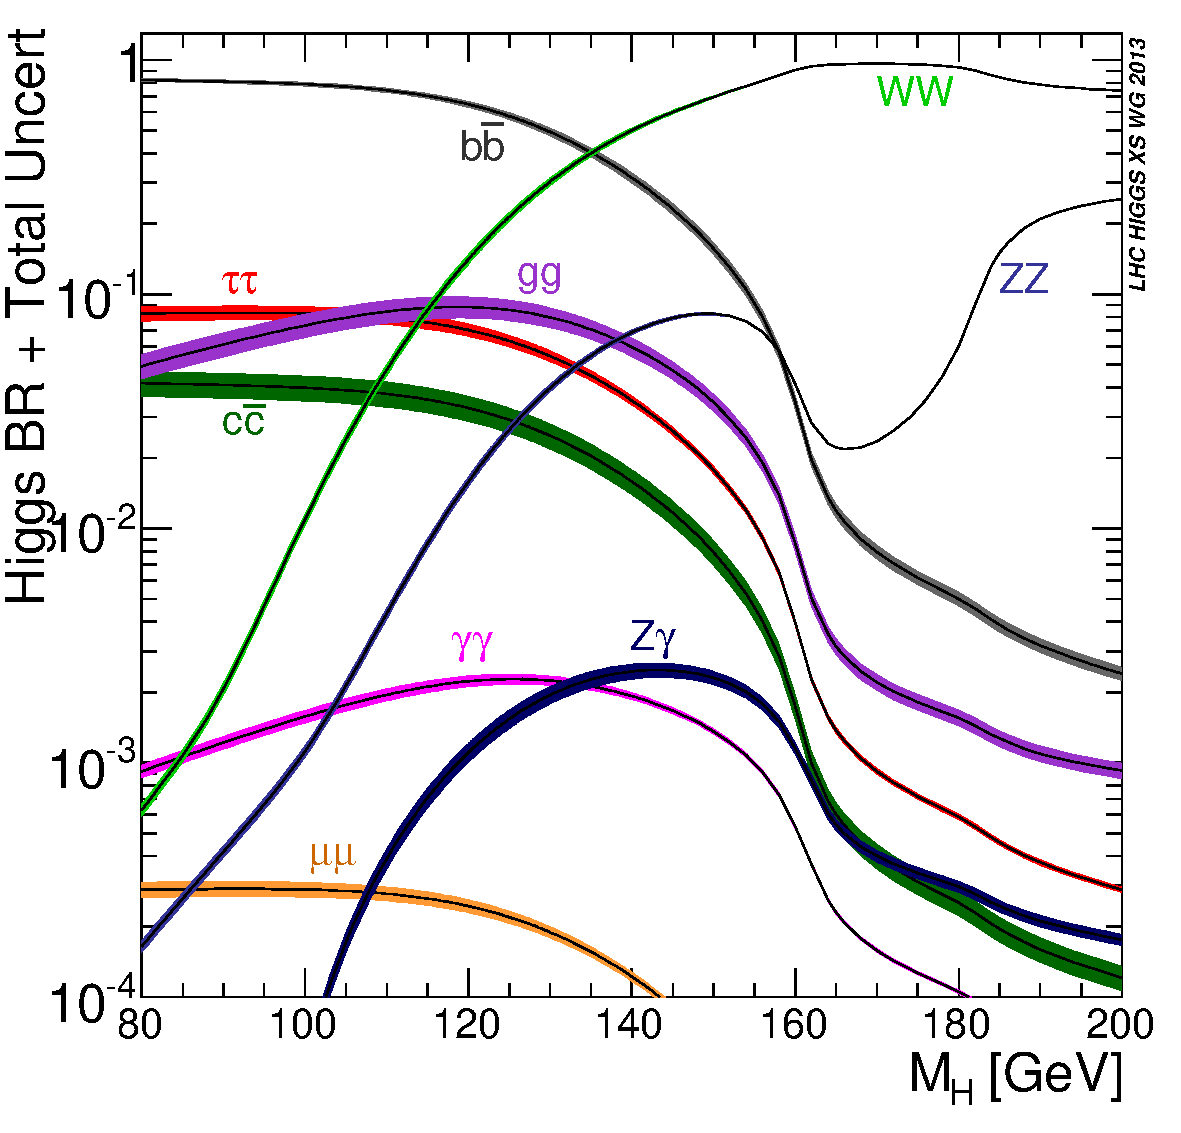
\includegraphics[width=0.48\textwidth]{figures/higgsmassmeas/higgs_BR_80to200GeV.pdf}
		\includegraphics[width=0.48\textwidth]{figures/higgsmassmeas/higgs_BR_120to130GeV.pdf}
		\caption{
            The branching ratios of various Higgs boson decays as a function of the Higgs boson mass
            over a wide range (Left) and a narrow range (Right) of values.
            }
		\label{fig:higgs_br}
	\end{center}
\end{figure} 
The question then becomes, \emph{``Which decay mode of the Higgs boson is most useful for the measurement of \mH?''}.
% Real particles enter detectors in CMS which send signals to various electronics.
% Particle Flow algorithm pieces the information together to construct objects out of each event.
% Now, instead of just a deposit of energy in the ECAL and corresponding hits in the silicon tracker, the particle is identified as a newly produced electron.
% CMS records which kinds of objects came from which events and stores the information in \emph{data sets} (TODO: ref Section future).

Owing to its large signal-to-background ratio of approximately 2 and its relatively rare four-lepton final state, the \hzzfourl decay channel is selected and is called the \emph{signal} process.
Thus, a single Higgs boson will decay via the signal process into two \PZ bosons (one on-shell and one off-shell) on average only 2.6\% of the time.
In turn, each \PZ boson decays into two opposite-sign, same flavor (OSSF) leptons (\Ztolplm, where $\ell = \Pe, \mu$) on average approximately 6.7\% of the time, giving rise to four distinct final states:
\foure, \fourmu, \twoetwomu, \twomutwoe.
The branching ratio for the overall signal process is then calculated as: % B(Z->ee)=0.033632, B(Z->mumu)=0.033662
\begin{equation*}
    \BRof{\hzzfourl} = \BRof{\htozz} \left[ \BRof{\Ztolplm} \right]^2 = 1.8\tentotheminus{3}.
\end{equation*}
Thus, a signal event is expected to be produced only once in about every \emph{trillion} \pp collisions.

The strategy is then to search the \pp collision data collected and analyzed by the CMS detector (Chapter~\ref{ch:cms_detector}) for all the detected \hzzfourl events.
The task is not so straightforward;
events in the data are categorized---not by the entire decay process---but by their final state, based on which triggers fired to collect which events.
Section~\ref{sec:datasets_simul_trig} describes the triggers used for this analysis to select events with the \fourl final state found in the corresponding data sets.
For each chosen event, the subdetectors of CMS (Chapter~\ref{ch:cms_detector}) provide a plethora of track and energy-detection information to reconstruct \emph{objects}---representations of the underlying particles within the event.
The reconstructed objects are then assembled in a fashion that checks if the logic coincides with the process of interest: \hzzfourl.  % TODO: Clean up this sentence.
For example, a pair of OSSF lepton-like objects should appear to come from a \PZ-like object---\ie having a nominal mass of approximately 91\GeV and zero net electric charge---instead of, say, appearing to come from a \PH-like object.
Two such \PZ-like objects must be formed and should appear to come from a \PH-like object.
% OSSF-dilepton objects should each appear to come from a \PZ-boson-like object (\eg having a nominal mass of approximately 91\GeV and zero net electric charge)---instead of, say, coming from a Higgs-boson-like object.
All throughout, the reconstructed event must obey physics conservation laws (energy, momentum, charge, \etc) and the associated objects may even be required to pass certain detector selection criteria (\eg $\pt^\mu > 5\GeV$).
% This process hinges on the conservation of momentum, since in the longitudinal ($z$) direction the \pp collision has initial and final.
% Specifically, the 
%     - The \PZ boson has a precisely measured mass of TODO a neutral particle, so the two leptons into which it decays should combine to Group two leptons together, 
%     - Form two different pairs of opposite-sign, same-flavor (OSSF) leptons
%     - If it appears that the to select specific hzz4l events (\emph{event selection}).
These criteria are analysis-specific and are collectively called the \emph{event selection} of the analysis.
The event selection for this analysis is described in Section~\ref{sec:evt_sel}.  % TODO: ref may be wrong.

Even though the event selection is constructed to select signal events, it is not guaranteed;
there are certain physics process that have exactly the same initial and final states as the signal process.
Such processes ``contaminate'' the collected signal events and are called \emph{background processes}.
Figure~\ref{TODO} shows how identical initial state gluons can react to produce exactly the same final state particles, while producing different intermediate particles:
the signal process (Left), initiated by gluon-gluon fusion \vs a background process (Right) which skips the intermediate Higgs boson.
It is imperative for all physics analyses to maximize the number of collected signal events while minimizing the number of collected background events.
Section~\ref{sec:bkg_estim} discusses the associated background processes and how to estimate the number of events these contribute to the signal region.
\begin{figure}[!htbp]
	\begin{center}
		\includegraphics[width=0.48\textwidth]{figures/placeholder.png}  % TODO.
		\includegraphics[width=0.48\textwidth]{figures/placeholder.png}  % TODO.
		\caption{
            Feynman diagrams showing how the initial and final states are the same
            for the signal process (\gghzzfourl, Left) and one possible background process (\ggzzfourl, Right).
        }
		\label{fig:feyndiag_sig_vs_bkg}
	\end{center}
\end{figure}

Before drawing conclusions from the data themselves, it is necessary for particle physicists to make predictions about their analysis using simulated samples or \emph{simulation}.
These samples contain simulated events usually of a specific process (\eg $\pp \to \hzzfourl$), governed by some theoretical framework that is programmed mathematically into the software package.
% events from simulated particle physics collisions--- are created by software physicists have created software packages that simulate particle physics collisions,
% the resulting particle transformations using various theoretical frameworks,
% and even the interactions that particles have with the virtual detectors, through which they traverse.
Programs like \MGvATNLO and \POWHEG can simulate millions of rare (or even \emph{fictitious}) events, which might otherwise take many years to observe in data.
Furthermore, software can even simulate the particles as they travel through the simulated detectors.
Programs like \GEANTfour can show analysts what to expect as the particles interact with a virtual version of the CMS detector.
Predictions from simulation can then be compared to the truth---the data---as a way to check the accuracy of the analysis.
For example, a surplus of events in data where none was expected may lead to the discovery of new particles, as was the case in the discovery of the Higgs boson.
% agreement or deviations in what was expected.
The simulated samples for this analysis are described in Section~\ref{sec:datasets_simul_trig}.

So how is the measurement of \mH achieved?
Since the signal process is \hzzfourl, conservation of energy leads one to expect that $\mH \approx \mfourl$.
Although this is not how the final measurement is obtained, it is a logical starting point.
The distribution of \mfourl values reveals the Higgs boson mass resonance (Figure~\ref{fig:m4l_run2}).
Simulation is then used to predict the \emph{line shape} of this signal peak (Section~\ref{sec:signal_model}).
This signal modeling is performed using a double-sided Crystal Ball function to fit the line shape, for various mass points of \mH, in each of the four final states.
% m4l dist Full Run 2.
%%%%%%%%%%%%%%%%%%%%
\begin{figure}[pbth]
    \centering
    \includegraphics[width=10cm,height=10cm,keepaspectratio]{figures/higgsmassmeas/m4l_FullRun2_epjc.jpeg}
        \caption{Distribution of \mfourl from \hzzfourl events using Full Run 2 data.}
        \label{fig:m4l_run2}
\end{figure}

In order to improve the precision of the measurement of \mH, several techniques are implemented.
The first technique is called the \Zone mass constraint, which uses the benefit of the mostly on-shell \Zone mass resonance to reevaluate the momenta of the leptons that went into building the \Zone.
This improves the lepton momentum resolution, thereby improving the resolution of the \mH peak.
The second technique is event-by-event mass uncertainty.
The third technique is vertex constraint.

% is mostly on-shell as opposed to the \Ztwo.
% Z1 significantly on-shell, but Z2 is mostly off-shell.
% 	- Therefore just perform constraint on mZ1.
% 	- Idea is to reevaluate the lepton
% - Per-event 

The resolution of the peak 
Ways to improve the 
Do likelihood fit.
$\mathcal{L}$
% \section{Analyzed Data}
\label{sec:analyzed_data}
The CMS experiment recorded LHC~\ref{ch:lhc} data during 2016, 2017, and 2018 (collectively called Run 2), corresponding to an integrated luminosity of \lumiruntwo.
These events were categorized by the trigger system~\ref{sec:trigger} into different data sets, depending on which triggers ``fired'', \ie whether the event passed the trigger criteria or not.
The names of the data sets are listed in Tables~\ref{table:2016_dataSamples}--\ref{table:2018_dataSamples} and follow the format \texttt{/object\_type/campaign/datatier}.
This analysis uses the ultra legacy (UL) reconstruction~\cite{}.
% TODO: Cite some UL source.
It should be noted that the 2016 data are split into 2 different reconstruction versions, starting at Run2016F:
the first version is ``pre-VFP'', which uses HIP mitigation (HIPM) in the reconstruction, and the second is ``post-VFP'', which uses the default reconstruction.

For the \hzzfourl analysis, Sec.~\ref{sec:trig} lists the triggers used, Sec.~\ref{sec:datasets} details the data sets used, and Sec.~\ref{sec:sim_samples} summarizes the simulated samples used.

% TODO:cite.
% \begin{itemize}
%     \item ``pre-VFP'', which uses HIP mitigation (HIPM) in the reconstruction
%     \item  ``post-VFP'', which uses the default reconstruction
% \end{itemize}
% TODO: Possibly convert data set names in table to monowidth. Do so with \texttt{}.
\subsection{Triggers}
\label{sec:trig}
%%%%%%%%%%%%%%%%%%%%%%%%%%%%%%%%%%%%%%%%%%%%%%%
%=== Triggers 2016 (for pre- and post-VFP) ===%
%%%%%%%%%%%%%%%%%%%%%%%%%%%%%%%%%%%%%%%%%%%%%%%
\begin{table}[!ht]
    % \small
    % \centering
    \topcaption
        [Trigger paths used to collect 2016 data (pre- and post-VFP)]
        {Trigger paths used to collect 2016 data (pre- and post-VFP) for the measurement of \mh.}
		\begin{tabular}{|lll|}
		\hline      
            HLT Path                                                        & Prescale          & Primary Data Set \\
        \hline
            % TODO: Confirm with Filippo that these paths are correct.
            % TODO: Where can I find all the list of triggers? How do we know these are the best triggers to use and that we didn't miss any?
            % The trigger paths below are from the Python script: templateData_UL16preVFP_10626_3l_cfg.py.
            % (A) = Found in AN-19-139v6.
            % (S) = Found in Python script.
            % * None of the AN paths do not contain "_v" at the end.
            % * I appended a "*" to the end of all "_v".
            \texttt{HLT\_DoubleEle33\_CaloIdL\_GsfTrkIdVL\_v*} & 1 & DoubleEG \\                        % (A) + (S)
            \texttt{HLT\_Ele16\_Ele12\_Ele8\_CaloIdL\_TrackIdL\_v*} & 1 & DoubleEG \\                   % (A) + (S)
            \texttt{HLT\_Ele17\_Ele12\_CaloIdL\_TrackIdL\_IsoVL\_DZ\_v*} & 1 & DoubleEG \\              % (A) + (S)
            \texttt{HLT\_Ele23\_Ele12\_CaloIdL\_TrackIdL\_IsoVL\_DZ\_v*} & 1 & DoubleEG \\              % (A) + (S)
            \texttt{HLT\_Mu17\_TrkIsoVVL\_Mu8\_TrkIsoVVL\_DZ\_v*} & 1 & DoubleMuon \\                   % (S)
            \texttt{HLT\_Mu17\_TrkIsoVVL\_Mu8\_TrkIsoVVL\_v*} & 1 & DoubleMuon \\                       % (A) + (S)
            \texttt{HLT\_Mu17\_TrkIsoVVL\_TkMu8\_TrkIsoVVL\_DZ\_v*} & 1 & DoubleMuon \\                 % (S)
            \texttt{HLT\_Mu17\_TrkIsoVVL\_TkMu8\_TrkIsoVVL\_v*} & 1 & DoubleMuon \\                     % (A) + (S)
            \texttt{HLT\_TripleMu\_12\_10\_5\_v*} & 1 & DoubleMuon \\                                   % (A) + (S)
            \texttt{HLT\_DiMu9\_Ele9\_CaloIdL\_TrackIdL\_v*} & 1 & MuonEG \\                            % (A) + (S)
            \texttt{HLT\_Mu8\_DiEle12\_CaloIdL\_TrackIdL\_v*} & 1 & MuonEG \\                           % (A) + (S)
            \texttt{HLT\_Mu8\_TrkIsoVVL\_Ele17\_CaloIdL\_TrackIdL\_IsoVL\_v*} & 1 & MuonEG \\           % (A) + (S)
            \texttt{HLT\_Mu8\_TrkIsoVVL\_Ele23\_CaloIdL\_TrackIdL\_IsoVL\_DZ\_v*} & 1 & MuonEG \\       % (S)
            \texttt{HLT\_Mu8\_TrkIsoVVL\_Ele23\_CaloIdL\_TrackIdL\_IsoVL\_v*} & 1 & MuonEG \\           % (A) + (S)
            \texttt{HLT\_Mu17\_TrkIsoVVL\_Ele12\_CaloIdL\_TrackIdL\_IsoVL\_v*} & 1 & MuonEG \\          % (A) + (S)
            \texttt{HLT\_Mu23\_TrkIsoVVL\_Ele8\_CaloIdL\_TrackIdL\_IsoVL\_v*} & 1 & MuonEG \\           % (A) + (S)
            \texttt{HLT\_Mu23\_TrkIsoVVL\_Ele12\_CaloIdL\_TrackIdL\_IsoVL\_DZ\_v*} & 1 & MuonEG \\      % (S)
            \texttt{HLT\_Mu23\_TrkIsoVVL\_Ele12\_CaloIdL\_TrackIdL\_IsoVL\_v*} & 1 & MuonEG \\          % (A) + (S)
            \texttt{HLT\_Ele25\_eta2p1\_WPTight\_Gsf\_v*} & 1 & SingleElectron \\                       % (S)
            \texttt{HLT\_Ele27\_eta2p1\_WPLoose\_Gsf\_v*} & 1 & SingleElectron \\                       % (A) + (S)
            % HLT_Ele25_eta2p1_WPTight                                                                  % (A)
            % HLT_Ele27_WPTight                                                                         % (A)
            \texttt{HLT\_Ele27\_WPTight\_Gsf\_v*} & 1 & SingleElectron \\                               % (S)
            \texttt{HLT\_Ele32\_eta2p1\_WPTight\_Gsf\_v*} & 1 & SingleElectron \\                       % (S)
            \texttt{HLT\_IsoMu20\_v* OR HLT\_IsoTkMu20\_v*} & 1 & SingleMuon \\                         % (A) + (S)
            \texttt{HLT\_IsoMu22\_v* OR HLT\_IsoTkMu22\_v*} & 1 & SingleMuon \\                         % (A) + (S)
            \texttt{HLT\_IsoMu24\_v* OR HLT\_IsoTkMu24\_v*} & 1 & SingleMuon \\                         % (S)
            %=== Duplicate of above but without backspaces.
            % \texttt{HLT_Ele16_Ele12_Ele8_CaloIdL_TrackIdL_v*} & 1 & DoubleEG \\             % (A) + (S)
            % \texttt{HLT_Ele17_Ele12_CaloIdL_TrackIdL_IsoVL_DZ_v*} & 1 & DoubleEG \\         % (A) + (S)
            % \texttt{HLT_Ele23_Ele12_CaloIdL_TrackIdL_IsoVL_DZ_v*} & 1 & DoubleEG \\         % (A) + (S)
            % \texttt{HLT_DoubleEle33_CaloIdL_GsfTrkIdVL_v*} & 1 & DoubleEG \\                % (A) + (S)
            % \texttt{HLT_Mu17_TrkIsoVVL_Mu8_TrkIsoVVL_v*} & 1 & DoubleMuon \\                % (A) + (S)
            % \texttt{HLT_Mu17_TrkIsoVVL_Mu8_TrkIsoVVL_DZ_v*} & 1 & DoubleMuon \\             % (S)
            % \texttt{HLT_Mu17_TrkIsoVVL_TkMu8_TrkIsoVVL_DZ_v*} & 1 & DoubleMuon \\           % (S)
            % \texttt{HLT_Mu17_TrkIsoVVL_TkMu8_TrkIsoVVL_v*} & 1 & DoubleMuon \\              % (A) + (S)
            % \texttt{HLT_TripleMu_12_10_5_v*} & 1 & DoubleMuon \\                            % (A) + (S)
            % \texttt{HLT_Mu8_TrkIsoVVL_Ele17_CaloIdL_TrackIdL_IsoVL_v*} & 1 & MuonEG \\      % (A) + (S)
            % \texttt{HLT_Mu8_TrkIsoVVL_Ele23_CaloIdL_TrackIdL_IsoVL_v*} & 1 & MuonEG \\      % (A) + (S)
            % \texttt{HLT_Mu8_TrkIsoVVL_Ele23_CaloIdL_TrackIdL_IsoVL_DZ_v*} & 1 & MuonEG \\   % (S)
            % \texttt{HLT_Mu17_TrkIsoVVL_Ele12_CaloIdL_TrackIdL_IsoVL_v*} & 1 & MuonEG \\     % (A) + (S)
            % \texttt{HLT_Mu23_TrkIsoVVL_Ele12_CaloIdL_TrackIdL_IsoVL_v*} & 1 & MuonEG \\     % (A) + (S)
            % \texttt{HLT_Mu23_TrkIsoVVL_Ele12_CaloIdL_TrackIdL_IsoVL_DZ_v*} & 1 & MuonEG \\  % (S)
            % \texttt{HLT_Mu23_TrkIsoVVL_Ele8_CaloIdL_TrackIdL_IsoVL_v*} & 1 & MuonEG \\      % (A) + (S)
            % \texttt{HLT_Mu8_DiEle12_CaloIdL_TrackIdL_v*} & 1 & MuonEG \\                    % (A) + (S)
            % \texttt{HLT_DiMu9_Ele9_CaloIdL_TrackIdL_v*} & 1 & MuonEG \\                     % (A) + (S)
            % \texttt{HLT_Ele25_eta2p1_WPTight_Gsf_v*} & 1 & SingleElectron \\                % (S)
            % \texttt{HLT_Ele27_WPTight_Gsf_v*} & 1 & SingleElectron \\                       % (S)
            % \texttt{HLT_Ele27_eta2p1_WPLoose_Gsf_v*} & 1 & SingleElectron \\                % (A) + (S)
            % \texttt{HLT_Ele32_eta2p1_WPTight_Gsf_v*} & 1 & SingleElectron \\                % (S)
            % \texttt{HLT_IsoMu20_v* OR HLT_IsoTkMu20_v*} & 1 & SingleMuon \\                 % (A) + (S)
            % \texttt{HLT_IsoMu22_v* OR HLT_IsoTkMu22_v*} & 1 & SingleMuon \\                 % (A) + (S)
            % \texttt{HLT_IsoMu24_v* OR HLT_IsoTkMu24_v*} & 1 & SingleMuon \\                 % (S)
        \hline
		\end{tabular}
	\label{table:2016_trig}
\end{table}
    % === ORIGINAL triggers found in both: templateData_UL16preVFP_10626_3l_cfg_FOR_Sync.py AND templateData_UL16postVFP_10626_3l_cfg_FOR_Sync.py
        % Also the same triggers as those found in:
        % * templateData_UL16preVFP_10612_2l_cfg.py
        % * templateData_UL16preVFP_10626_3l_cfg_FOR_Sync.py
        %===
        % HLT_Ele17_Ele12_CaloIdL_TrackIdL_IsoVL_DZ_v
        % HLT_Ele23_Ele12_CaloIdL_TrackIdL_IsoVL_DZ_v
        % HLT_DoubleEle33_CaloIdL_GsfTrkIdVL_v
        % HLT_Mu17_TrkIsoVVL_Mu8_TrkIsoVVL_DZ_v
        % HLT_Mu17_TrkIsoVVL_TkMu8_TrkIsoVVL_DZ_v
        % HLT_Mu17_TrkIsoVVL_Mu8_TrkIsoVVL_v
        % HLT_Mu17_TrkIsoVVL_TkMu8_TrkIsoVVL_v
        % HLT_Mu8_TrkIsoVVL_Ele17_CaloIdL_TrackIdL_IsoVL_v
        % HLT_Mu8_TrkIsoVVL_Ele23_CaloIdL_TrackIdL_IsoVL_v
        % HLT_Mu8_TrkIsoVVL_Ele23_CaloIdL_TrackIdL_IsoVL_DZ_v
        % HLT_Mu17_TrkIsoVVL_Ele12_CaloIdL_TrackIdL_IsoVL_v
        % HLT_Mu23_TrkIsoVVL_Ele12_CaloIdL_TrackIdL_IsoVL_v
        % HLT_Mu23_TrkIsoVVL_Ele12_CaloIdL_TrackIdL_IsoVL_DZ_v
        % HLT_Mu23_TrkIsoVVL_Ele8_CaloIdL_TrackIdL_IsoVL_v
        % HLT_Mu8_DiEle12_CaloIdL_TrackIdL_v
        % HLT_DiMu9_Ele9_CaloIdL_TrackIdL_v
        % HLT_Ele16_Ele12_Ele8_CaloIdL_TrackIdL_v
        % HLT_TripleMu_12_10_5_v
        % HLT_Ele25_eta2p1_WPTight_Gsf_v
        % HLT_Ele27_WPTight_Gsf_v
        % HLT_Ele27_eta2p1_WPLoose_Gsf_v
        % HLT_Ele32_eta2p1_WPTight_Gsf_v
        % HLT_IsoMu20_v
        % HLT_IsoTkMu20_v
        % HLT_IsoMu22_v
        % HLT_IsoTkMu22_v
        % HLT_IsoMu24_v
        % HLT_IsoTkMu24_v
        %=== From AN-19-139v6.
        % HLT_Ele17_Ele12_CaloIdL_TrackIdL_IsoVL_DZ
        % HLT_Ele23_Ele12_CaloIdL_TrackIdL_IsoVL_DZ
        % HLT_DoubleEle33_CaloIdL_GsfTrkIdVL
        % HLT_Ele16_Ele12_Ele8_CaloIdL_TrackIdL
        % HLT_Mu17_TrkIsoVVL_Mu8_TrkIsoVVL
        % HLT_Mu17_TrkIsoVVL_TkMu8_TrkIsoVVL
        % HLT_TripleMu_12_10_5
        % HLT_Mu8_TrkIsoVVL_Ele17_CaloIdL_TrackIdL_IsoVL
        % HLT_Mu8_TrkIsoVVL_Ele23_CaloIdL_TrackIdL_IsoVL
        % HLT_Mu17_TrkIsoVVL_Ele12_CaloIdL_TrackIdL_IsoVL
        % HLT_Mu23_TrkIsoVVL_Ele12_CaloIdL_TrackIdL_IsoVL
        % HLT_Mu23_TrkIsoVVL_Ele8_CaloIdL_TrackIdL_IsoVL
        % HLT_Mu8_DiEle12_CaloIdL_TrackIdL
        % HLT_DiMu9_Ele9_CaloIdL_TrackIdL
        % HLT_Ele25_eta2p1_WPTight
        % HLT_Ele27_WPTight
        % HLT_Ele27_eta2p1_WPLoose_Gsf
        % HLT_IsoMu20 OR HLT_IsoTkMu20
        % HLT_IsoMu22 OR HLT_IsoTkMu22
%%%%%%%%%%%%%%%%%%%%%%%
%=== Triggers 2017 ===%
%%%%%%%%%%%%%%%%%%%%%%%
\begin{table}[!ht]	
    % \small
    % \centering
    \topcaption
        [Trigger paths used to collect 2017 data]
        {Trigger paths used to collect 2017 data for the measurement of \mh.}
		\begin{tabular}{|lll|}
		\hline      
        HLT Path                                                        & Prescale          & Primary Data Set \\
        \hline
            % TODO: Confirm with Filippo that these paths are correct.
            % TODO: Where can I find all the list of triggers? How do we know these are the best triggers to use and that we didn't miss any?
            % The trigger paths below are from the Python script: templateData_UL17_10626_4l_cfg_FOR_Sync.py.
            % (A) = Found in AN-19-139v6.
            % (S) = Found in Python script.
            % There are only a couple differences compared to those found in AN-19-139v6:
            % * Most of the AN paths do not contain "_v" at the end.
            % * HLT_DoubleEle33_CaloIdL* has a different suffix.
            % * I appended a "*" to the end of all "_v".
            \texttt{HLT\_DoubleEle33\_CaloIdL\_MW\_v*}                       & 1 &                  DoubleEG  \\ % (S)
            \texttt{HLT\_Ele16\_Ele12\_Ele8\_CaloIdL\_TrackIdL\_v*}          & 1 &                  DoubleEG  \\  % (A) + (S)
            \texttt{HLT\_Ele23\_Ele12\_CaloIdL\_TrackIdL\_IsoVL\_v*}         & 1 &                  DoubleEG  \\  % (A) + (S)
            % 'HLT\_DoubleEle33\_CaloIdL\_GsfTrkIdVL',                                                         % (A)  \\
            \texttt{HLT\_Mu17\_TrkIsoVVL\_Mu8\_TrkIsoVVL\_DZ\_Mass3p8\_v*}           & 1 &          DoubleMuon  \\  % (A) + (S)
            \texttt{HLT\_Mu17\_TrkIsoVVL\_Mu8\_TrkIsoVVL\_DZ\_Mass8\_v*}         & 1 &              DoubleMuon  \\  % (A) + (S)
            \texttt{HLT\_TripleMu\_10\_5\_5\_DZ\_v*}         & 1 &                                  DoubleMuon  \\  % (A) + (S)
            \texttt{HLT\_TripleMu\_12\_10\_5\_v*}            & 1 &                                  DoubleMuon  \\  % (A) + (S)
            \texttt{HLT\_DiMu9\_Ele9\_CaloIdL\_TrackIdL\_DZ\_v*}         & 1 &                      MuonEG  \\  % (A) + (S)
            \texttt{HLT\_Mu8\_DiEle12\_CaloIdL\_TrackIdL\_DZ\_v*}            & 1 &                  MuonEG  \\  % (A) + (S)
            \texttt{HLT\_Mu8\_DiEle12\_CaloIdL\_TrackIdL\_v*}            & 1 &                      MuonEG  \\  % (A) + (S)
            \texttt{HLT\_Mu8\_TrkIsoVVL\_Ele23\_CaloIdL\_TrackIdL\_IsoVL\_DZ\_v*}            & 1 &  MuonEG  \\  % (A) + (S)
            \texttt{HLT\_Mu12\_TrkIsoVVL\_Ele23\_CaloIdL\_TrackIdL\_IsoVL\_DZ\_v*}           & 1 &  MuonEG    \\  % (A) + (S)
            \texttt{HLT\_Mu23\_TrkIsoVVL\_Ele12\_CaloIdL\_TrackIdL\_IsoVL\_DZ\_v*}           & 1 &  MuonEG     \\  % (A) + (S)
            \texttt{HLT\_Mu23\_TrkIsoVVL\_Ele12\_CaloIdL\_TrackIdL\_IsoVL\_v*}           & 1 &      MuonEG  \\  % (A) + (S)
            \texttt{HLT\_Ele35\_WPTight\_Gsf\_v*}            & 1 &                                  SingleElectron  \\  % (A) + (S)
            \texttt{HLT\_Ele38\_WPTight\_Gsf\_v*}            & 1 &                                  SingleElectron  \\  % (A) + (S)
            \texttt{HLT\_Ele40\_WPTight\_Gsf\_v*}            & 1 &                                  SingleElectron  \\  % (A) + (S)
            \texttt{HLT\_IsoMu27\_v*}            & 1 &                                              SingleMuon  \\  % (A) + (S)
        \hline
    %=== From AN-19-139v6.
    % HLT_Ele23_Ele12_CaloIdL_TrackIdL_IsoVL_*
    % HLT_DoubleEle33_CaloIdL_GsfTrkIdVL
    % HLT_Ele16_Ele12_Ele8_CaloIdL_TrackIdL
    % HLT_Mu17_TrkIsoVVL_Mu8_TrkIsoVVL_DZ_Mass3p8
    % HLT_Mu17_TrkIsoVVL_Mu8_TrkIsoVVL_DZ_Mass8
    % HLT_TripleMu_12_10_5
    % HLT_TripleMu_10_5_5_DZ
    % HLT_Mu23_TrkIsoVVL_Ele12_CaloIdL_TrackIdL_IsoVL
    % HLT_Mu8_TrkIsoVVL_Ele23_CaloIdL_TrackIdL_IsoVL_DZ
    % HLT_Mu12_TrkIsoVVL_Ele23_CaloIdL_TrackIdL_IsoVL_DZ
    % HLT_Mu23_TrkIsoVVL_Ele12_CaloIdL_TrackIdL_IsoVL_DZ
    % HLT_DiMu9_Ele9_CaloIdL_TrackIdL_DZ
    % HLT_Mu8_DiEle12_CaloIdL_TrackIdL
    % HLT_Mu8_DiEle12_CaloIdL_TrackIdL_DZ
    % HLT_Ele35_WPTight_Gsf_v*
    % HLT_Ele38_WPTight_Gsf_v*
    % HLT_Ele40_WPTight_Gsf_v*
    % HLT_IsoMu27
    %=== ORIGINAL templateData_UL17_10626_4l_cfg_FOR_Sync.py:
    % 'HLT_Ele23_Ele12_CaloIdL_TrackIdL_IsoVL_v',
    % 'HLT_DoubleEle33_CaloIdL_MW_v',
    % 'HLT_Mu17_TrkIsoVVL_Mu8_TrkIsoVVL_DZ_Mass3p8_v',
    % 'HLT_Mu17_TrkIsoVVL_Mu8_TrkIsoVVL_DZ_Mass8_v',
    % 'HLT_Mu23_TrkIsoVVL_Ele12_CaloIdL_TrackIdL_IsoVL_v',
    % 'HLT_Mu8_TrkIsoVVL_Ele23_CaloIdL_TrackIdL_IsoVL_DZ_v',
    % 'HLT_Mu12_TrkIsoVVL_Ele23_CaloIdL_TrackIdL_IsoVL_DZ_v',
    % 'HLT_Mu23_TrkIsoVVL_Ele12_CaloIdL_TrackIdL_IsoVL_DZ_v',
    % 'HLT_DiMu9_Ele9_CaloIdL_TrackIdL_DZ_v',
    % 'HLT_Mu8_DiEle12_CaloIdL_TrackIdL_v',
    % 'HLT_Mu8_DiEle12_CaloIdL_TrackIdL_DZ_v',
    % 'HLT_Ele16_Ele12_Ele8_CaloIdL_TrackIdL_v',
    % 'HLT_TripleMu_10_5_5_DZ_v',
    % 'HLT_TripleMu_12_10_5_v',
    % 'HLT_Ele35_WPTight_Gsf_v',
    % 'HLT_Ele38_WPTight_Gsf_v',
    % 'HLT_Ele40_WPTight_Gsf_v',
    % 'HLT_IsoMu27_v',
		\end{tabular}
	\label{table:2018_trig}
\end{table}
%%%%%%%%%%%%%%%%%%%%%%%
%=== Triggers 2018 ===%
%%%%%%%%%%%%%%%%%%%%%%%
\begin{table}[!ht]	
    % \small
    % \centering
    \topcaption
        [Trigger paths used to collect 2018 data]
        {Trigger paths used to collect 2018 data for the measurement of \mh.}
		\begin{tabular}{|lcl|}
		\hline      
        HLT Path                                                        & Prescale          & Primary Data Set \\
        \hline
        % TODO: Confirm with Filippo that these paths are correct.
        % TODO: Where can I find all the list of triggers? How do we know these are the best triggers to use and that we didn't miss any?
            % The trigger paths below are from the Python script: templateData_UL18_10626_3l_cfg_FOR_SYNC.py.
            % (A) Found in AN-19-139v6.
            % (T) Toni used these triggers in the script.
            % There are only a couple differences compared to those found in AN-19-139v6:
            % * Most of the AN paths do not contain "_v" at the end.
            % * HLT_DoubleEle33_CaloIdL* has a different suffix.
            % * I appended a "*" to the end of all "_v".
            \texttt{HLT\_DoubleEle25\_CaloIdL\_MW\_v*}                              & 1                 & DoubleEG              \\  % (A) & (T)
            \texttt{HLT\_Ele23\_Ele12\_CaloIdL\_TrackIdL\_IsoVL\_v*}                & 1                 & DoubleEG           \\  % (A) & (T)
            \texttt{HLT\_Mu17\_TrkIsoVVL\_Mu8\_TrkIsoVVL\_DZ\_Mass3p8\_v*}          & 1                 & DoubleMuon               \\  % (A) & (T)
            \texttt{HLT\_TripleMu\_10\_5\_5\_DZ\_v*}                              & 1                   & DoubleMuon             \\  % (T)
            \texttt{HLT\_TripleMu\_12\_10\_5\_v*}                                & 1                    & DoubleMuon            \\  % (T)
            \texttt{HLT\_DiMu9\_Ele9\_CaloIdL\_TrackIdL\_DZ\_v*}                  & 1                   & MuonEG          \\  % (A) & (T)
            \texttt{HLT\_Mu8\_DiEle12\_CaloIdL\_TrackIdL\_DZ\_v*}                 & 1                   & MuonEG               \\  % (T)
            \texttt{HLT\_Mu8\_DiEle12\_CaloIdL\_TrackIdL\_v*}                    & 1                    & MuonEG              \\  % (T)
            \texttt{HLT\_Mu8\_TrkIsoVVL\_Ele23\_CaloIdL\_TrackIdL\_IsoVL\_DZ\_v*}   & 1                 & MuonEG                \\  % (A) & (T)
            \texttt{HLT\_Mu12\_TrkIsoVVL\_Ele23\_CaloIdL\_TrackIdL\_IsoVL\_DZ\_v*}  & 1                 & MuonEG          \\  % (A) & (T)
            \texttt{HLT\_Mu23\_TrkIsoVVL\_Ele12\_CaloIdL\_TrackIdL\_IsoVL\_DZ\_v*}  & 1                 & MuonEG                \\  % (T)
            \texttt{HLT\_Mu23\_TrkIsoVVL\_Ele12\_CaloIdL\_TrackIdL\_IsoVL\_v*}      & 1                 & MuonEG          \\  % (A) & (T)
            \texttt{HLT\_Ele32\_WPTight\_Gsf\_v*}                               & 1                     & SingleElectron    \\  % (A) & (T)
            \texttt{HLT\_IsoMu24\_v*}                                         & 1                       & SingleMuon    \\  % (A) & (T)
        \hline
        %=== ORIGINAL templateData_UL18_10626_3l_cfg_FOR_SYNC.py
        % Toni
        % 'HLT_Ele32_WPTight_Gsf_v', 
        % 'HLT_IsoMu24_v',
        % 'HLT_Ele23_Ele12_CaloIdL_TrackIdL_IsoVL_v',
        % 'HLT_DoubleEle25_CaloIdL_MW_v',
        % 'HLT_Mu17_TrkIsoVVL_Mu8_TrkIsoVVL_DZ_Mass3p8_v',
        % 'HLT_Mu23_TrkIsoVVL_Ele12_CaloIdL_TrackIdL_IsoVL_v',
        % 'HLT_Mu8_TrkIsoVVL_Ele23_CaloIdL_TrackIdL_IsoVL_DZ_v',
        % 'HLT_Mu12_TrkIsoVVL_Ele23_CaloIdL_TrackIdL_IsoVL_DZ_v',
        % 'HLT_Mu23_TrkIsoVVL_Ele12_CaloIdL_TrackIdL_IsoVL_DZ_v',
        % 'HLT_DiMu9_Ele9_CaloIdL_TrackIdL_DZ_v',
        % 'HLT_TripleMu_10_5_5_DZ_v',
        % 'HLT_TripleMu_12_10_5_v',
        % 'HLT_Mu8_DiEle12_CaloIdL_TrackIdL_v', 
        % 'HLT_Mu8_DiEle12_CaloIdL_TrackIdL_DZ_v', 
		\end{tabular}
	\label{table:2018_trig}
\end{table}
% % HIG-19-001 shows these triggers:
% HLT_Ele17_Ele12_CaloIdL_TrackIdL_IsoVL_DZ
% HLT_Ele23_Ele12_CaloIdL_TrackIdL_IsoVL_DZ

% % From: templateData_102X_4l_cfg.py
% # Single Lepton:
% 'HLT_Ele35_WPTight_Gsf',
% 'HLT_Ele38_WPTight_Gsf',
% 'HLT_Ele40_WPTight_Gsf',
% 'HLT_IsoMu27',
% # Dilepton
% 'HLT_Ele23_Ele12_CaloIdL_TrackIdL_IsoVL',
% 'HLT_DoubleEle33_CaloIdL_MW',
% 'HLT_Mu17_TrkIsoVVL_Mu8_TrkIsoVVL_DZ_Mass3p8',
% 'HLT_Mu17_TrkIsoVVL_Mu8_TrkIsoVVL_DZ_Mass8',
% 'HLT_Mu23_TrkIsoVVL_Ele12_CaloIdL_TrackIdL_IsoVL',
% 'HLT_Mu8_TrkIsoVVL_Ele23_CaloIdL_TrackIdL_IsoVL_DZ',
% 'HLT_Mu12_TrkIsoVVL_Ele23_CaloIdL_TrackIdL_IsoVL_DZ',
% 'HLT_Mu23_TrkIsoVVL_Ele12_CaloIdL_TrackIdL_IsoVL_DZ',
% 'HLT_DiMu9_Ele9_CaloIdL_TrackIdL_DZ',
% 'HLT_Mu8_DiEle12_CaloIdL_TrackIdL',
% 'HLT_Mu8_DiEle12_CaloIdL_TrackIdL_DZ',
% # TriLepton
% 'HLT_Ele16_Ele12_Ele8_CaloIdL_TrackIdL',
% 'HLT_TripleMu_10_5_5_DZ',
% 'HLT_TripleMu_12_10_5',

\subsection{Data Sets}
\label{sec:datasets}
% TODO: Should this be split into pre and post-VFP?
%=== Data sets 2016.
\begin{table}[!ht]	
    %  \captionsetup{justification=justified}
    \small
    \centering
    \topcaption
        [Data sets used for 2016 UL]
        {Names and integrated luminosities $\left( \lumiint \right)$ of the 2016 UL data sets, where $\text{(1)} = \text{MINIAOD}$.}
		\begin{tabular}{|lc|}
		\hline      
        Data Set Name & \lumiint (\fbinv) \\
        %$\left( \fbinv \right)$ 
        \hline
        % TODO: Update Lints.
        /DoubleEG/Run2016B-ver1\_HIPM\_UL2016\_MiniAODv2-v1/(1) & \multirow{5}{*}{TODO} \\
        /DoubleMuon/Run2016B-ver1\_HIPM\_UL2016\_MiniAODv2-v1/(1)	& \\
        /SingleElectron/Run2016B-ver1\_HIPM\_UL2016\_MiniAODv2-v2/(1)	& \\
        /SingleMuon/Run2016B-ver1\_HIPM\_UL2016\_MiniAODv2-v2/(1)	& \\
        /MuonEG/Run2016B-ver1\_HIPM\_UL2016\_MiniAODv2-v2/(1)	& \\
        \hline
        /DoubleEG/Run2016B-ver2\_HIPM\_UL2016\_MiniAODv2-v3/(1) & \multirow{5}{*}{TODO} \\
        /DoubleMuon/Run2016B-ver2\_HIPM\_UL2016\_MiniAODv2-v1/(1)	& \\
        /SingleElectron/Run2016B-ver2\_HIPM\_UL2016\_MiniAODv2-v2/(1)	& \\
        /SingleMuon/Run2016B-ver2\_HIPM\_UL2016\_MiniAODv2-v2/(1)	& \\
        /MuonEG/Run2016B-ver2\_HIPM\_UL2016\_MiniAODv2-v2/(1)	& \\
        \hline
        /DoubleEG/Run2016C-HIPM\_UL2016\_MiniAODv2-v1/(1) & \multirow{5}{*}{TODO} \\
        /DoubleMuon/Run2016C-HIPM\_UL2016\_MiniAODv2-v1/(1)	& \\
        /SingleElectron/Run2016C-HIPM\_UL2016\_MiniAODv2-v2/(1)	& \\
        /SingleMuon/Run2016C-HIPM\_UL2016\_MiniAODv2-v2/(1)	& \\
        /MuonEG/Run2016C-HIPM\_UL2016\_MiniAODv2-v2/(1)	& \\
        \hline
        /DoubleEG/Run2016D-HIPM\_UL2016\_MiniAODv2-v1/(1) & \multirow{5}{*}{TODO} \\
        /DoubleMuon/Run2016D-HIPM\_UL2016\_MiniAODv2-v1/(1)	& \\
        /SingleElectron/Run2016D-HIPM\_UL2016\_MiniAODv2-v2/(1)	& \\
        /SingleMuon/Run2016D-HIPM\_UL2016\_MiniAODv2-v2/(1)	& \\
        /MuonEG/Run2016D-HIPM\_UL2016\_MiniAODv2-v2/(1)	& \\
        \hline
        /DoubleEG/Run2016E-HIPM\_UL2016\_MiniAODv2-v1/(1) & \multirow{5}{*}{TODO} \\
        /DoubleMuon/Run2016E-HIPM\_UL2016\_MiniAODv2-v1/(1)	& \\
        /SingleElectron/Run2016E-HIPM\_UL2016\_MiniAODv2-v5/(1)	& \\
        /SingleMuon/Run2016E-HIPM\_UL2016\_MiniAODv2-v2/(1)	& \\
        /MuonEG/Run2016E-HIPM\_UL2016\_MiniAODv2-v2/(1)	& \\
        \hline
        /DoubleEG/Run2016F-HIPM\_UL2016\_MiniAODv2-v1/(1) & \multirow{5}{*}{TODO} \\
        /DoubleMuon/Run2016F-HIPM\_UL2016\_MiniAODv2-v1/(1)	& \\
        /SingleElectron/Run2016F-HIPM\_UL2016\_MiniAODv2-v2/(1)	& \\
        /SingleMuon/Run2016F-HIPM\_UL2016\_MiniAODv2-v2/(1)	& \\
        /MuonEG/Run2016F-HIPM\_UL2016\_MiniAODv2-v2/(1)	& \\
        \hline
        /DoubleEG/Run2016F-UL2016\_MiniAODv2-v1/(1) & \multirow{5}{*}{TODO} \\
        /DoubleMuon/Run2016F-UL2016\_MiniAODv2-v1/(1)	& \\
        /SingleElectron/Run2016F-UL2016\_MiniAODv2-v2/(1)	& \\
        /SingleMuon/Run2016F-UL2016\_MiniAODv2-v2/(1)	& \\
        /MuonEG/Run2016F-UL2016\_MiniAODv2-v2/(1)	& \\
        \hline
        /DoubleEG/Run2016G-UL2016\_MiniAODv2-v1/(1) & \multirow{5}{*}{TODO} \\
        /DoubleMuon/Run2016G-UL2016\_MiniAODv2-v1/(1)	& \\
        /SingleElectron/Run2016G-UL2016\_MiniAODv2-v2/(1)	& \\
        /SingleMuon/Run2016G-UL2016\_MiniAODv2-v2/(1)	& \\
        /MuonEG/Run2016G-UL2016\_MiniAODv2-v2/(1)	& \\
        \hline
        /DoubleEG/Run2016H-UL2016\_MiniAODv2-v1/(1) & \multirow{5}{*}{TODO} \\
        /DoubleMuon/Run2016H-UL2016\_MiniAODv2-v2/(1)	& \\
        /SingleElectron/Run2016H-UL2016\_MiniAODv2-v2/(1)	& \\
        /SingleMuon/Run2016H-UL2016\_MiniAODv2-v2/(1)	& \\
        /MuonEG/Run2016H-UL2016\_MiniAODv2-v2/(1)	& \\
        \hline
		\end{tabular}
	\label{table:2016_dataSamples}
\end{table}
%=== Data sets 2017.
\begin{table}[!ht]	
    %  \captionsetup{justification=justified}
    \small
    \centering
    \topcaption
        [UL data sets used for 2017]
        {Names of the UL 2017 data sets and the corresponding integrated luminosities $\left( \lumiint \right)$. $\text{(1)} = \text{MINIAOD}$}
		\begin{tabular}{|lc|}
		\hline      
        Data Set Name & Integrated Luminosity (\fbinv) \\
        %$\left( \fbinv \right)$ 
        \hline
        % TODO: Update Lints.
        /SingleMuon/Run2017B-UL2017\_MiniAODv2-v1/(1) & \multirow{5}{*}{TODO} \\
        /SingleElectron/Run2017B-UL2017\_MiniAODv2-v1/(1)	&	\\
        /DoubleMuon/Run2017B-UL2017\_MiniAODv2-v1/(1)	&	\\
        /DoubleEG/Run2017B-UL2017\_MiniAODv2-v1/(1)	&	\\
        /MuonEG/Run2017B-UL2017\_MiniAODv2-v1/(1)	&	\\
        \hline
        /SingleMuon/Run2017C-UL2017\_MiniAODv2-v1/(1) & \multirow{5}{*}{TODO} \\
        /SingleElectron/Run2017C-UL2017\_MiniAODv2-v1/(1)	& \\
        /DoubleMuon/Run2017C-UL2017\_MiniAODv2-v1/(1)	& \\
        /DoubleEG/Run2017C-UL2017\_MiniAODv2-v1/(1)	& \\
        /MuonEG/Run2017C-UL2017\_MiniAODv2-v1/(1)	& \\
        \hline
        /SingleElectron/Run2017D-UL2017\_MiniAODv2-v1/(1) & \multirow{5}{*}{TODO} \\
        /SingleMuon/Run2017D-UL2017\_MiniAODv2-v1/(1)	& \\
        /DoubleMuon/Run2017D-UL2017\_MiniAODv2-v1/(1)	& \\
        /DoubleEG/Run2017D-UL2017\_MiniAODv2-v1/(1)	& \\
        /MuonEG/Run2017D-UL2017\_MiniAODv2-v1/(1)	& \\
        \hline
        /SingleElectron/Run2017E-UL2017\_MiniAODv2-v1/(1) & \multirow{5}{*}{TODO} \\
        /SingleMuon/Run2017E-UL2017\_MiniAODv2-v1/(1)	& \\
        /DoubleMuon/Run2017E-UL2017\_MiniAODv2-v2/(1)	& \\
        /DoubleEG/Run2017E-UL2017\_MiniAODv2-v1/(1)	& \\
        /MuonEG/Run2017E-UL2017\_MiniAODv2-v1/(1)	& \\
        \hline
        /SingleElectron/Run2017F-UL2017\_MiniAODv2-v1/(1) & \multirow{5}{*}{TODO} \\
        /SingleMuon/Run2017F-UL2017\_MiniAODv2-v1/(1)	& \\
        /DoubleMuon/Run2017F-UL2017\_MiniAODv2-v1/(1)	& \\
        /DoubleEG/Run2017F-UL2017\_MiniAODv2-v1/(1)	& \\
        /MuonEG/Run2017F-UL2017\_MiniAODv2-v1/(1)	& \\
        \hline	
		\end{tabular}
	\label{table:2017_dataSamples}
\end{table}
%=== Data sets 2018.
\begin{table}[!ht]	
    %  \captionsetup{justification=justified}
    \small
    \centering
    \topcaption
    [UL data sets used for 2018]
    {Names of the UL 2018 data sets and the corresponding integrated luminosities $\left( \lumiint \right)$. $\text{(1)} = \text{MINIAOD}$}
		\begin{tabular}{|lc|}
		\hline      
        Data Set Name & Integrated Luminosity (\fbinv) \\
        %$\left( \fbinv \right)$ 
        \hline
        % TODO: Update Lints.
		/SingleMuon/Run2018A-UL2018\_MiniAODv2-v3/(1) & \multirow{4}{*}{TODO} \\
		/DoubleMuon/Run2018A-UL2018\_MiniAODv2-v1/(1) & \\
		/EGamma/Run2018A-UL201\_MiniAODv2-v1/(1) & \\
		/MuonEG/Run2018A-UL2018\_MiniAODv2-v1/(1) & \\
		\hline
		/SingleMuon/Run2018B-UL2018\_MiniAODv2-v2/(1) & \multirow{4}{*}{TODO} \\
		/DoubleMuon/Run2018B-UL2018\_MiniAODv2-v1/(1)	&  \\
		/EGamma/Run2018B-UL2018\_MiniAODv2-v1/(1)	&	\\
		/MuonEG/Run2018B-UL2018\_MiniAODv2-v1/(1)	&	\\
		\hline
		/SingleMuon/Run2018C-UL2018\_MiniAODv2-v2/(1) & \multirow{4}{*}{TODO} \\
		/DoubleMuon/Run2018C-UL2018\_MiniAODv2-v1/(1)	&	\\
		/EGamma/Run2018C-UL2018\_MiniAODv2-v1/(1)	&	\\
		/MuonEG/Run2018C-UL2018\_MiniAODv2-v1/(1)	&	\\
		\hline
		/SingleMuon/Run2018D-UL2018\_MiniAODv2-v3/(1) & \multirow{4}{*}{TODO} \\
		/DoubleMuon/Run2018D-UL2018\_MiniAODv2-v1/(1)	&	\\
		/EGamma/Run2018D-UL2018\_MiniAODv2-v1/(1)	&	\\
		/MuonEG/Run2018D-UL2018\_MiniAODv2-v1/(1)	&	\\
		\hline	
		\end{tabular}
	\label{table:2018_dataSamples}
\end{table}


\subsection{Simulated Events}
% Monte Carlo refers to a simulation technique.
% Therefore "Monte Carlo events" makes no sense, while "Monte Carlo program" is fine.
% Use "simulated events" instead (NOT "simulation" samples!).
\label{sec:sim_samples}

% % This section was Event Reconstruction and Selection but now just making it Event Selection.
\section{Object and Event Selection}
\label{sec:evt_sel}
Amidst the chaotic particle deluge that arises from \pp collisions, those events which appear to follow the decay chain and properties of the \hzzfourl signal must be carefully selected.
Crafting a well-designed \emph{event selection} that identifies these signal events---while throwing away the nonsignal events---is the goal.
By implementing a rigorous
trigger selection,
vertex selection,
final-state object selection,
and \ZZ-candidate selection,
the purity of the signal process is optimized and---by extension---so is the precision on the measurement of \mH.

As part of the event selection, the particle objects themselves must pass certain kinematical criteria to be considered for the analysis.
The object selection used in this analysis is summarized in \cref{table:obj_sel_higgs} and the step-by-step event selection can be found in Ref.~\cite{HIG_19_001}.
% TODO: Change all tables to tabularx?
\begin{table}\fontsize{10}{12}\selectfont\centering\renewcommand{\arraystretch}{2}
    \captionof{table}
        [Object selection criteria for \mH measurement analysis]
        {Object selection criteria for \mH measurement analysis.}
    \begin{tabularx}{\textwidth}{>{\hsize=.3\hsize}X>{\hsize=.2\hsize}c>{\hsize=.2\hsize}c>{\hsize=.3\hsize}X}
        \toprule
        \multicolumn{4}{c}
            {\textbf{Electrons}} \\
                \hline
            & $\pte > 7\GeV$ & $\absetaof{\Pe} < 2.5$ & \\
            & $d_{xy} < 0.5\cm$ & $d_{z} < 1\cm$ & \\
        \multicolumn{4}{c}{$|\text{SIP}_\text{3D}| < 4$} \\
        \multicolumn{4}{c}{Satisfies BDT ID from isolation cuts found in Ref.~\cite{HIG_19_001}} \\
        \toprule

        \multicolumn{4}{c}{\textbf{Muons}} \\
            \hline
        \multicolumn{4}{c}{Global or Tracker Muon} \\
        \multicolumn{4}{c}{Discard Standalone Muon tracks if reconstructed in muon system only} \\
            & $\ptmu > 5\GeV$ & $\absetaof{\Pmu} < 2.4$ & \\
            & $d_{xy} < 0.5\cm$ & $d_{z} < 1\cm$ & \\
        \multicolumn{4}{c}{$|\text{SIP}_\text{3D}| < 4$} \\
        \multicolumn{4}{c}{PF muon ID if $\ptmu < 200\GeV$, PF muon ID or High-$\pT$ muon ID if $\ptmu > 200\GeV$ according to (Ref.~\cite{HIG_19_001})}\\
        \multicolumn{4}{c}{$\mathcal{I}_\text{PF}^\Pmu < 0.35$} \\
        \toprule
        
        \multicolumn{4}{c}{\textbf{FSR Photons}} \\ \hline
        & $\frac{\Delta R(\ell,\gamma)}{\left( \pT^\gamma \right)^2}$$\pT^\gamma > 2\GeV$ & $\absetaof{\gamma} < 2.4$ & \\
        \multicolumn{4}{c}{$\mathcal{I}_\text{PF}^\gamma < 1.8$} \\ 
        & $\Delta R(\ell,\gamma) < 0.5$ & $\frac{\Delta R(\ell,\gamma)}{\left( \pT^\gamma \right)^2} < 0.012\GeV^{-2}$ & \\
        \toprule

        \multicolumn{4}{c}{\textbf{Jets}} \\ \hline
        & $\pT^\text{jet} > 30\GeV$ & $\absetaof{\text{jet}} < 4.7$ & \\
        \multicolumn{4}{c}{$\Delta R(\ell/\gamma, \text{jet}) > 0.4$} \\
        \multicolumn{4}{c}{Cut-based jet ID (tight WP)} \\
        \multicolumn{4}{c}{Jet pileup ID (tight WP)} \\
        \multicolumn{4}{c}{Deep CSV \Pqb-tagging (medium WP)} \\ \toprule
    \end{tabularx}
    \label{table:obj_sel_higgs}
\end{table}

After the full analysis selection is implemented in each of the \fourl final states and the distributions are shown in \cref{fig:m4l_dists}.
The expected yields for the signal and background processes are given in \cref{tab:yield_sr_105to140,tab:yield_sr_70to170},
which count events within the narrow signal region $\left(105 < \mfourl < 140\GeV\right)$ and wide signal region $\left(70 < \mfourl < 170\GeV\right)$, respectively.
\begin{multiFigure}
    \centering
        \addFigure{0.48}{../../higgsmassmeasurement/AN-19-248/Figures/MassDistribution_70_170/InclusiveMass_4mu_workinprogress.pdf}
        \addFigure{0.48}{../../higgsmassmeasurement/AN-19-248/Figures/MassDistribution_70_170/InclusiveMass_4e_workinprogress.pdf}
        \addFigure{0.48}{../../higgsmassmeasurement/AN-19-248/Figures/MassDistribution_70_170/InclusiveMass_2e2mu_workinprogress.pdf}
        \addFigure{0.48}{../../higgsmassmeasurement/AN-19-248/Figures/MassDistribution_70_170/InclusiveMass_2mu2e_workinprogress.pdf}
        \addFigure{0.75}{../../higgsmassmeasurement/AN-19-248/Figures/MassDistribution_70_170/InclusiveMass_workinprogress.pdf}
    \captionof{figure}
        [Distributions of the four-lepton invariant mass]
        {Distributions of the four-lepton invariant mass, inclusively and by final state.
        \;A) Events with the \fourmu final state.
        \;B) Events with the \foure final state.
        \;C) Events with the \twoetwomu final state.
        \;D) Events with the \twomutwoe final state.
        \;E) All final states included.}
    \label{fig:m4l_dists}
\end{multiFigure}
\begin{table}[!htb]
    \centering
    \topcaption
        [Yields in the narrow signal region $105 < \mfourl < 140\GeV$]
        {Number of expected yields of signal and background processes within the narrow signal region $105 < \mfourl < 140\GeV$ after the full event selection using \lumiruntwo, split into the four final states.}
    \begin{tabular}{lrrrrr}
        \hline
    Process                                 & \fourmu   & \foure    & \twoetwomu    & \twomutwoe    & Inclusive    \\
        \hline
    \qqzzfourl                              &   88.8    &   38.5    & 63.7          &   41.8        &   232.8   \\
    \ggzzfourl                              &   9.7     &   4.8     & 4.8           &   3.7         &   23.0    \\
    RB                                      &   32.4    &   12.2    & 29.2          &  18.6         &   92.4    \\
    Sum of Background                       &   130.9   &   55.5    & 97.7          & 64.1          &   348.2   \\
        \hline
    Signal $\left( \mH = 125\GeV \right)$   &   90.5    &   48.2    & 64.6          & 53.0          &   256.3   \\
        \hline
    Total Expected                          &   221.4   & 103.7     & 162.3         & 117.1         &   604.5   \\
        \hline
    \end{tabular}
    \label{tab:yield_sr_105to140}
\end{table}
\begin{table}[!htb]
    \centering
    \topcaption
        [Yields in the wide signal region $70 < \mfourl < 170\GeV$]
        {Number of expected yields of signal and background processes within the wide signal region $70 < \mfourl < 170\GeV$ after the full event selection using \lumiruntwo, split into the four final states.}
    \begin{tabular}{lrrrrr}
        \hline
    Process                                 &   \fourmu &   \foure  &   \twoetwomu  &   \twomutwoe  &   Inclusive   \\
        \hline
    \qqzzfourl                              &   486.7   &   192.0   &   246.0       &   170.1       &   1094.9      \\
    \ggzzfourl                              &   29.7	&   15.2	&   13.3	    &   12.2	    &   70.5        \\
    RB                                      &   70.1    &   30.3    &	61.5        &	42.2	    &   204.1       \\
    Sum of Background                       &   586.5   &	237.5	&   320.8	    &   224.5	    &   1369.3      \\
        \hline
    Signal $\left( \mH = 125\GeV \right)$   &  92.4     &   49.6    &   66.5        &   54.3        &   262.8       \\ 
        \hline
    Total Expected                          &  679.0    &	287.2	&   387.4	    &   278.8	    &   1632.3      \\
        \hline
    \end{tabular}
    \label{tab:yield_sr_70to170}
\end{table}

% \section{Signal Modeling}
\label{sec:signal_model}
%=== FROM AN but modified. ===%
%The dominant POWHEG ggF process is reweighted to the NNLOPS one, using bins of generated Higgs 
%$p_{T}$ and number of generated jets. More details in \cite{HIG_19_001}.
% TODO:REWORD

\subsection{Signal Normalization}
\label{sec:SignalNormalization}
% TODO:REWORD
The normalization of the Higgs boson signal is obtained from simulation, 
looking at the expected signal yields in the range [105, 140] GeV, 
for five simulated mass points (120, 124, 125, 126, and 130 GeV).
A second order polynomial function is used to extract the dependence of the normalization from $m_{H}$.
Fits are performed separately for each production mode, for each decay channel and for each year. 
Examples of the fits are shown in Fig.~\ref{fig:signal_normalization}
\begin{multiFigure}
    \centering
        \addFigure{0.48}{../../higgsmassmeasurement/AN-19-248/Figures/SignalModelling/Signal_Normalisation/NoZ1/2016pre_ggH_yield_workinprogress.pdf}
        \addFigure{0.48}{../../higgsmassmeasurement/AN-19-248/Figures/SignalModelling/Signal_Normalisation/NoZ1/2016post_ggH_yield_workinprogress.pdf}
        \addFigure{0.48}{../../higgsmassmeasurement/AN-19-248/Figures/SignalModelling/Signal_Normalisation/NoZ1/2017_ggH_yield_workinprogress.pdf}
        \addFigure{0.48}{../../higgsmassmeasurement/AN-19-248/Figures/SignalModelling/Signal_Normalisation/NoZ1/2018_ggH_yield_workinprogress.pdf}
    \captionof{figure}
        [Normalization fit for the ggH signal in different final states]
        {Normalization fit for the ggH signal in different final states (expected yield \vs $\mH / 125\GeV$) for all years during Run 2.
        \;A) 2016 pre-VFP.
        \;B) 2016 post-VFP.
        \;C) 2017.
        \;D) 2018.}
    \label{fig:signal_normalization}
\end{multiFigure}

\subsection{Parameterizing the Signal Line Shape}
\label{sec:SignalParametrization}
% TODO:REWORD
The signal lineshape is obtained from the fit of the Higgs boson mass distribution, 
in the range [105, 140]\GeV, using a double-sided Crystal Ball (DSCB) function, which has 6 parameters.
%This function has six independent parameters, 
%with a Gaussian core ($\sigma_{m}$) that describes the four-lepton mass resolution function and 
%the systematic mass shift ($\Delta m_{H}$) of the peak, and the left- and right-hand tail 
%originating from leptons emitting brem in the tracker material, present for both electrons and muons, 
%and from the non-Gaussian mis-measurements specific to interactions of electrons with the detector material 
%(each side of the distribution is described by two parameters, n and $\alpha$).\\
Fit parameters $\theta^i$ are derived as a function of \mH, using a first-order polynomial:
%\textbf{Compare first vs second order formula: current results with second one}
\[
\theta^{i}_\text{DSCB} = a^i + b^{i}~(\mH - 125)% + c~(m_{H} - 125)^{2}
\]

First, fitting only the 125\GeV sample, the $a^i$ term for each parameter is extracted ($b^i$ is not yet taken into account).
Then, a second fit is performed:
this time, $a^i$ is fixed to the value found before, while $b^i$ is kept free to float when fitting all five different mass points (120, 124, 125, 126, 130\GeV) simultaneously.

The fit is performed separately, for each production mode, for each decay channel, for each year. 
To take into account the non-resonant contribution in the case of $\PV\PH$ and $\ttbarh$ production modes, the 
DSCB is convoluted with a Landau function that describes the possibility for a 
lepton from the Higgs boson decay to be lost or not selected.\\
\subsection{Building the 1D pdf}
The measurement of \mH is extracted by maximizing the one-dimensional likelihood function $\lhood \left( \mH \middlepipe \mfourl \right)$ using the \mfourl spectrum.  % TODO: Filippo has: "where $m_{H}$ is fixed to the value of 125 GeV." but this doesn't make sense. 
The model and the normalization used for the signal are described in Sec.~\ref{sec:SignalNormalization}.
The DSCB fits of the four-lepton invariant mass distributions are shown in Figure.~\ref{fig:1D_mass_2018_ggH} for the signal region 105--140\GeV using simulated ggH events, split into the four different final states.
% TODO: 2017 or 2016 plots?
\begin{multiFigure}
    \centering
        \addFigure{0.48}{../../higgsmassmeasurement/AN-19-248/Figures/ggH_MassDistribution/1D_mass_2018_ggH_4mu_workinprogress.pdf}
        \addFigure{0.48}{../../higgsmassmeasurement/AN-19-248/Figures/ggH_MassDistribution/1D_mass_2018_ggH_4e_workinprogress.pdf}
        \addFigure{0.48}{../../higgsmassmeasurement/AN-19-248/Figures/ggH_MassDistribution/1D_mass_2018_ggH_2e2mu_workinprogress.pdf}
        \addFigure{0.48}{../../higgsmassmeasurement/AN-19-248/Figures/ggH_MassDistribution/1D_mass_2018_ggH_2mu2e_workinprogress.pdf}
    \captionof{figure}
        [Distributions of \mfourl in the signal region (105--140\GeV) using simulated ggH events]
        {Distributions of \mfourl in the signal region (105--140\GeV) using simulated ggH events, fitted with a DSCB function using 2018 samples.
        \;A) \fourmu.
        \;B) \foure.
        \;C) \twoetwomu.
        \;D) \twomutwoe.}
    \label{fig:1D_mass_2018_ggH}
\end{multiFigure}

\subsubsection{Expected uncertainties on \mH before improvements}
Assuming perfect background rejection and neglecting any systematic uncertainties, the expected uncertainty on the measurement of \mH is shown in Tables~\ref{table:1D_model_result_fs} and~\ref{table:1D_model_result_year}, split by final state and by year, respectively.
% TODO: Consider using tabularx
%=== By final state.
\begin{table}[!ht]
    % \small
    \centering
    \topcaption
        [Expected Higgs boson mass uncertainty measured with the 1D model]
        {Expected Higgs boson mass uncertainty measured with the 1D model for different final states.
        All mass uncertainties are reported in $\MeVns$ and are statistical-only.
        }
	\begin{tabular}{cccccc}
            \hline      
        Expected uncertainty $(\MeVns)$	&	\fourmu	&	\foure	&	\twoetwomu	& \twomutwoe	& Inclusive	\\
            \hline
        1D	(No bkg) &	147	&	394	&	276	&	273	&	112	\\
            \hline
        \end{tabular}
    \label{table:1D_model_result_fs}
\end{table}
%=== By year.
\begin{table}[!ht]
    % \small
    \centering
    \topcaption
        [Expected Higgs boson mass uncertainty measured with the 1D model]
        {Expected Higgs boson mass uncertainty measured with the 1D model for different years during Run 2.
        All mass uncertainties are reported in $\MeVns$ and are statistical-only.
        }
	\begin{tabular}{|ccccc|}
            \hline      
        Expected uncertainty $(\MeVns)$	&	2016 pre-VFP	&	2016 post-VFP	&	2017	&	2018	\\
            \hline
        1D (No bkg)	&	304	&	314	&	207	&	170	\\
            \hline
        \end{tabular}
    \label{table:1D_model_result_year}
\end{table}
% TODO: Include any of the below?
%The 1D likelihood scans vs \mH, while profiling signal strength $\mu$ as all other nuisance parameters, are 
%shown in \figurename~\ref{1D_model}. 
%%All systematic errors are included. In order to estimate the 
%%contribution of the statistical and systematic error to the mass measurement, a likelihood scan removing 
%%both the normalization and shape systematics is performed. As in the case of the scan including the full 
%%uncertainties, $\mu$ is profiled, and then its uncertainty is included in the statistical error, because 
%%its magnitude represents the amount of signal events fitted, and then it has statistical nature. 
%%The systematic uncertainty is estimated as the difference in quadrature between the full uncertainty 
%%and the statistical uncertainty. 
%Results are summarised in ~\tablename~\ref{table:1D_model_result}.
% \section{Techniques to Improve Mass Resolution}
\label{sec:techniques}
Words!
% \section{Background Estimation}
\label{sec:bkg_estim}
Measurement of the Higgs boson mass requires the accurate modeling of the total event yield in the signal region (SR), into which events can be categorized as either \emph{signal} or \emph{background}.
These background events pass the signal event selection
% TODO: (Sec.~\ref{sec:zz_sel})
and thus spoil the purity of the signal events.
This introduces further uncertainty into the final Higgs boson mass measurement.
Therefore, it is a priority to reduce and to predict the expected number of background events, which can be split into two types: \emph{irreducible background} (IB) and \emph{reducible background} (RB) processes.

\subsection{Irreducible Background}
\label{sec:bkg_irred}
IB processes produce two \PZ bosons and each \PZ subsequently decays into two prompt leptons (leptons that emerge directly from the primary vertex).
This reliably produces a \fourl final state, whose prompt leptons are typically reconstructed as four leptons that pass tight selection (\emph{PTS leptons}), as defined in Sec.~\ref{sec:evt_sel}.
The IB event then looks indistinguishable from the 4 PTS lepton of the \emph{signal} process and cannot be reduced;
Thus, throwing away IB process could mean throwing away a signal event.
Since IB events cannot be completely eliminated---or \emph{reduced}---from the SR, they are given the name \emph{irreducible} backgrounds.
The two IBs for this analysis are:
\begin{itemize}
    \item \ggzzfourl (gluon-gluon fusion),
    \item \qqzzfourl (quark-antiquark annihilation).
\end{itemize}

\subsubsection{ggZZ background}
Following the prescription from Ref.~\cite{HIG_19_001}, the \ggzzfourl background is reweighted by a $K$ factor to reach NNLO precision.

\subsubsection{qqZZ background}
%qqZZ with k.qqZZ.ewk and k.qqZZ.qcd.M
The \qqzzfourl background is generated at NLO and then scaled to NNLO using NNLO/NLO $K$ factors,
as a function of \mass{\ZZ}. Additional NLO electroweak corrections, which depend on the initial state quark flavors and their
kinematic variables, are also applied to this process in the region $\mass{\ZZ} > 2\mass{\PZ}$, where the corrections have been computed. 
For more details and plots, see Ref.~\cite{HIG_19_001}.

\subsection{Reducible Background}
\label{sec:redbkg}
While IB processes produce 4 prompt leptons, RB processes produce varying numbers of prompt and nonprompt leptons.
Nonprompt leptons emerge from 3 main sources:
\begin{itemize}
    \item misidentifying light-flavor hadrons (\eg $\pi^{\pm}$) as leptons
    \item heavy-flavor hadrons that decay mid-flight into leptons
    \item the asymmetric conversion of photons into electrons
\end{itemize}

This analysis is tailored to efficiently reconstruct prompt(nonprompt) leptons as PTS(FTS) leptons.
Ideally, the SR would contain only the events with 4 prompt leptons, which would always be tagged as 4 PTS leptons.
However, sometimes a truly nonprompt lepton is misidentified as a PTS lepton (sometimes called a \emph{fake lepton}), depending on the kinematic properties of the lepton.
This misidentification rate ($f$, sometimes called the \emph{fake rate}) is due to imperfect detector performance, inefficiencies in reconstruction, and the specific choice of lepton selections used in the analysis.

If an event produces prompt and nonprompt leptons but is reconstructed as 4 PTS leptons (a 4P event), then it contaminates the SR.
These processes constitute the RB processes (sometimes called ``\ZplusX'').
Examples of RB processes for this analysis include:
\begin{itemize}
	\item \Zplusjets (yields 2 prompt leptons)
	\item \ttbarplusjets (yields 2 prompt leptons)
	\item \WZplusjets (yields 3 prompt leptons)
	\item $\ZZ/\Zgammastar + \text{jets}$ (yields 4 prompt leptons).
\end{itemize}
The careful estimation of these RB contributions to the 4P region is necessary for the precise measurement of the Higgs boson mass.

\subsubsection{OS Method}
\label{sec:os_method}
The goal of the OS Method is to estimate the number of opposite-sign same-flavor (OSSF) \fourl events produced by RB process that ``contaminate'' the 4P region $\left( \nfourPRB \right)$, given by Eq.~\ref{eqn:rbe_formula_final}.
% Since the $4\ell$ final state of the signal process consists of 2 pairs of OSSF leptons, the method is called the \emph{OS Method}.
However, the typical approach of using simulated samples does not model RB well, since RB processes (\eg \Zplusjets) rely on higher-order effects like jet modelling which are not yet accurately simulated.
Instead, a data-driven approach is used.

The logic of the OS Method is to study events in data that are similar to, but not exactly the same as, those found in the 4P region.
Thus, events in data are sorted into 2 control regions (CRs), both of which are orthogonal to the 4P region and to each other:
\begin{itemize}
	\item the \emph{3P1F} CR (built from 3 PTS and 1 FTS leptons)
	\item the \emph{2P2F} CR (built from 2 PTS and 2 FTS leptons).
\end{itemize}
The event selection for the 2P2F and 3P1F CRs is almost identical to that of the SR, % TODO:REF TO EVT SEL %Sec.~\ref{sec:zz_sel}),
except that the FTS lepton(s) are required to build the \Ztwo.
The events that contribute mostly to the 2P2F(3P1F) CR are those that produce 2(3) prompt and 2(1) nonprompt leptons and are called \emph{2pr}(\emph{3pr}) events.
Similarly, the events that contribute mostly to the 4P SR are those that produce 4 prompt leptons and are called \emph{4pr} events.

The final formula for \nfourPRB is obtained by first supposing that event $k$ is a 2pr event and contributes to the 2P2F CR an event weight of $\wgttwoprompttotwoPtwoF^k$.
This weight is built from $\hat{w}^k$, which is the product of analysis weights (pileup, L1 pre-firing, \etc), and the reconstruction efficiencies ($\epsilon$) of each lepton ($\ell_n$):
\begin{equation}
	\label{eqn:wt_2prto2p2f}
	\wgttwoprompttotwoPtwoF^k = \hat{w}^k \cdot \effprpass(\ell_1^k) \cdot \effprpass(\ell_2^k) \cdot \effnpfail(\ell_3^k) \cdot \effnpfail(\ell_4^k),
\end{equation}
where the superscript of $\epsilon$ indicates the lepton promptness (pr = prompt, np = nonprompt),
the subscript indicates the lepton tightness status (P = PTS, F = FTS).
To simplify the equations that follow, $\hat{w}^k$ is set to unity.
%  \effprpass(\ell_1^k) is the efficiency of reconstructing $\ell_1$ from event $k$ as a \mathbf{P}TS lepton
% and \effnpfail(\ell_3^k) is the efficiency of reconstructing $\ell_3$ from event $k$ as a \mathbf{F}TS lepton
% where $\epsilon^{\mathrm{pr|np}}_{\mathrm{P|F}}$ is the efficiency of reconstructing a prompt/nonprompt lepton passing/failing tight selections.
If the reconstruction efficiencies of a particular category are the same for all $j$ leptons across all $k$ events $\left( \eg ~ \effprpass(\ell_j^k) \equiv \effprpass \right)$, then Eq.~\ref{eqn:wt_2prto2p2f} reduces to:
\begin{equation}
	\label{eqn:wt_2prto2p2f_simp}
	\wgttwoprompttotwoPtwoF^k = 
	\left( \effprpass \right)^2 
	\left( \effnpfail \right)^2.
\end{equation}

Although a 2pr event mostly contributes to the 2P2F CR, a nonprompt lepton may be misidentified as a PTS lepton, depending on \effnppass.
Such an event would then fall into the 3P1F CR and, allowing for only one nonprompt PTS lepton at a time, contributes an effective weight of
\begin{align}
	\label{eqn:wt_2prto3p1f}
	\wgttwoprompttothreePoneF^k
	&= \left( \effprpass \right)^2 
	\left[
		\effnppass(\ell_1^k) \cdot \effnpfail(\ell_2^k) + \effnpfail(\ell_1^k) \cdot \effnppass(\ell_2^k)
	\right]
	\notag
	\\
	&= \left( \effprpass \right)^2
	\left[
		2 \effnppass \effnpfail
	\right].
\end{align}
Using the fact that a (non)prompt lepton is exclusively either PTS or FTS
$\left( \epsilon^\text{pr(np)}_\text{P} + \epsilon^\text{pr(np)}_\text{F} = 1 \right)$,
% \begin{equation*}
% 	\epsilon^\mathrm{pr(np)}_\mathrm{P} + \epsilon^\mathrm{pr(np)}_\mathrm{F} = 1,
% \end{equation*}
while recognizing that $\effnppass \equiv f$ (Sec.~\ref{sec:redbkg}) and defining $\effprpass \equiv \epsilon$,
allows Eq.~\ref{eqn:wt_2prto3p1f} to be written as
\begin{equation}
	\label{eqn:wt_2prto3p1f_simp}
	\wgttwoprompttothreePoneF^k = 2 \epsilon^2 f (1-f).
\end{equation}
The prediction of Eq.~\ref{eqn:wt_2prto3p1f_simp} can be seen in Figs.~\ref{cr_plots_3p1f_2016prevfp}--\ref{cr_plots_3p1f_2018} (red line) for 2016--2018 UL data.

Even more rarely, both nonprompt leptons from a 2pr event may be misidentified as PTS leptons.
In this case, event $k$ contributes to the 4P region an effective weight of
\begin{equation}
	\label{eqn:wt_2prto4p}
	\wgttwoprompttofourP^k = \epsilon^2 f^2,
\end{equation}
where it is assumed that both leptons have the same misidentification rate.
Similar equations can be derived for the contributions of a 3pr event to the 3P1F CR and to the 4P region:
\begin{align}
	\label{eqn:wt_3prto3p1f}
	\wgtthreeprompttothreePoneF^k &= \epsilon^3 \left( 1-f \right)
	\\
	\label{eqn:wt_3prto4p}
	\wgtthreeprompttofourP^k &= \epsilon^3 f.
\end{align}
Since a 3pr event needs only 1 nonprompt PTS lepton to be included in the 4P region (therefore, carrying only 1 factor of $f$), a 3pr event tends to contribute more weight to 4P than does a 2pr event (which carries $f^2$).

If the total number of 2pr, 3pr, and 4pr events is \xtwoprompt, \xthreeprompt, and \xfourprompt, respectively, then Fig.~\ref{fig:prompt_to_crs} shows how the weight of a single event, derived in the previous equations (and others forthcoming), from each category contributes to the final yield of each CR $\left( \ntwoPtwoF, \nthreePoneF \right)$ and of the SR $\left( \nfourP \right)$.

% TODO: use consistent symbols in figure below!
\begin{figure}
	\centering
    \begin{tikzpicture}
        % top nodes
        \node[yshift=5pt] (X2pr) {$X_\text{2pr}$ {\small (Z + jets, $t\bar{t}$ + jets)}};
        \node[right=3.5cm of X2pr] (X3pr) {$X_\text{3pr}$ {\small(WZ + jets)}};
        \node[right=4.5cm of X3pr] (X4pr) {$X_\text{4pr}$ {\small(ZZ,Z$\gamma^*$)}};
        
        % bottom nodes
        \node[below=5.5cm of X2pr.west, xshift=12pt] (N2P2F) {$N_\text{2P2F}$};
        \node[below=5.5cm of X3pr.west, xshift=12pt] (N3P1F) {$N_\text{3P1F}$};
        \node[below=5.5cm of X4pr.west, xshift=12pt] (N4P) {$N_\text{4P}$};
        
        % solid lines
        \draw[-stealth, line width=1.5pt] ([yshift=-10pt,xshift=12pt]X2pr.west) -- (N2P2F);
        \draw[-stealth, line width=1.5pt] ([yshift=-10pt,xshift=12pt]X2pr.west) -- (N3P1F);
        \draw[-stealth, line width=1.5pt] ([yshift=-10pt,xshift=12pt]X2pr.west) -- (N4P);

        % dashed lines
        \draw[-stealth, dash pattern=on 10pt off 10pt, line width=1.5pt] ([yshift=-10pt,xshift=12pt]X3pr.west) -- (N3P1F);
        \draw[-stealth, dash pattern=on 10pt off 10pt, line width=1.5pt] ([yshift=-10pt,xshift=12pt]X3pr.west) -- (N4P);
        
        % dotted lines
        \draw[-stealth, loosely dotted, line width=2pt] ([yshift=-10pt,xshift=12pt]X4pr.west) -- (N3P1F);
        \draw[-stealth, loosely dotted, line width=2pt] ([yshift=-10pt,xshift=12pt]X4pr.west) -- (N4P);
        
        % equation nodes
        \node[draw, fill=white, below=4.15 of X2pr.west, xshift=12pt] (eq1) {\small $\epsilon^2(1-f)^2$};
        \node[draw, fill=white, below left=4.15 and 1.25cm of X3pr.west, xshift=12pt] (eq2) {\small $2\epsilon^2f(1-f)$};
        \node[draw, fill=white, below=4.15 of X3pr.west, xshift=10pt] (eq3) {\small $\epsilon^3(1-f)$};
        \node[draw, fill=white, below right=4.15 and 1.2cm of X3pr.west, xshift=12pt] (eq4) {\small $4\epsilon^3\epsilon_\text{F}^\text{pr}$};
        \node[draw, fill=white, below left=4.15 and 3.2cm of X4pr.west, xshift=12pt] (eq5) {\small $\epsilon^2f^2$};
        \node[draw, fill=white, below left=4.15 and 1.4cm of X4pr.west, xshift=12pt] (eq6) {\small $\epsilon^3f$};
        \node[draw, fill=white, below=4.15 of X4pr.west, xshift=12pt] (eq7) {\small $\epsilon^4$};

        % RB and IB nodes
        \node[fill=white, above=.25cm of eq5, yshift=-3pt] (RB) {\small RB};
        \node[fill=white, above left=.25cm and 0.25cm of eq7, yshift=-3pt] (IB) {\small IB};

        \draw[line width=1pt] ([yshift=2pt]RB.south) -- (eq5.north);
        \draw[line width=1pt] ([yshift=2pt]RB.south) -- (eq6.west);
        \draw[line width=1pt] ([yshift=2pt,xshift=4pt]IB.south) -- (eq7.west);
        
        % \draw[line width=1.5pt, -stealth] (e21f2) -- (N2P2F);
        
        % \diagram* {
            % (X2pr) -- (e21f2),
        %     (ZZ) -- [boson, edge label=$Z$] (Z1),
        %     (ZZ) -- [boson, edge label=$Z$] (Z2),
        %     (Z1) -- [boson, edge label=$Z_D$] (ZD),
        %     (ZDl2) -- [fermion] (ZD) -- [fermion] (ZDl1);
        %     (Z2l2) -- [fermion] (Z2) -- [fermion] (Z2l1);
        % };
    \end{tikzpicture}
	\caption
		[Diagram showing how RB prompt-lepton processes contribute to observed PTS-lepton events.]
		{Contributions of per-event weights (boxed values) of various $n$-prompt-lepton processes ($X_{n\text{pr}}$, in parentheses) to the total numbers of events in the observed control regions $\left( \ntwoPtwoF, \nthreePoneF \right)$ and signal region $\left( \nfourP \right)$.
		The labels ``IB'' and ``RB'' indicate those contributions which comprise the irreducible and reducible backgrounds, respectively.}
		\label{fig:prompt_to_crs}
\end{figure}

It is then straightforward to evaluate the expected number of RB 4P events:
\begin{align}
	\label{eqn:n4p_x2x3}
	\nfourPRB
	&= \sum_{k=1}^{\xtwoprompt} \wgttwoprompttofourP^k + \sum_{m=1}^{\xthreeprompt} \wgtthreeprompttofourP^m
	\notag
	\\
	&= \sum_{k=1}^{\xtwoprompt} \epsilon^2 f^2 + \sum_{m=1}^{\xthreeprompt} \epsilon^3 f
	\notag
	\\
	&= f^2 \epsilon^2 \xtwoprompt + f \epsilon^3 \xthreeprompt,
\end{align}
where only the quantities $f$ and $\epsilon$ are known, so \xtwoprompt and \xthreeprompt must be estimated.
This is achieved by relating \xtwoprompt to \ntwoPtwoF using Eq.~\ref{eqn:wt_2prto2p2f_simp} across all 2pr events:
% If the total number of true 2pr events is \xtwoprompt, then the expected number of 2P2F events $\left( \ntwoPtwoF \right)$ is obtained via Eq.:
\begin{align}
	\label{eqn:n2p2f_x2}
	\ntwoPtwoF
	&= \sum_{k=1}^{\xtwoprompt} \wgttwoprompttotwoPtwoF^k
	\notag
	\\
	% &= \sum_{k=1}^{\xtwoprompt} \epsilon^2 \left( \effnpfail \right)^2
	% \\
	&= \sum_{k=1}^{\xtwoprompt} \epsilon^2 \left( 1-f \right)^2
	\notag
	\\
	&= \left( 1-f \right)^2 \epsilon^2 \xtwoprompt
	% \\
	% \implies \xtwoprompt &= \frac{ \ntwoPtwoF }{ \epsilon^2 \left( 1-f \right)^2 }
\end{align}

The strategy to relate \xthreeprompt to \nthreePoneF is not as straightforward as relating \xtwoprompt to \ntwoPtwoF,
since two other sources also contribute to the 3P1F CR (as shown in Fig.~\ref{fig:prompt_to_crs}):
\begin{itemize}
	\item A 2pr RB process can yield one nonprompt PTS lepton (via Eq.~\ref{eqn:wt_2prto3p1f_simp}).
	\item A 4-prompt IB process (\qqggzzfourl, ``\ZZ'') can yield one FTS lepton.
\end{itemize}
The second of these is well estimated from simulation, since \ZZ produces 4 prompt leptons.
If the total number of simulated \ZZ events is \xfourpromptzz, then event $k$ belonging to these events contributes to the 3P1F CR an effective weight of
\begin{equation}
	\label{eqn:wt_4przzto3p1f}
	\wgtfourpromptzztothreePoneF^k = 4 \epsilon^3 \effprfail,
\end{equation}
which accounts for any of the 4 prompt leptons to be reconstructed as a FTS lepton while the others are PTS leptons.
Incorporating Eqs.~\ref{eqn:wt_2prto3p1f_simp},~\ref{eqn:wt_3prto3p1f}, and~\ref{eqn:wt_4przzto3p1f} for all events relates \xthreeprompt to \nthreePoneF:
\begin{align}
	\label{eqn:n3p1f_x3}
	\nthreePoneF
	&= \sum_{j=1}^{\xthreeprompt} \wgtthreeprompttothreePoneF^j + \sum_{k=1}^{\xtwoprompt} \wgttwoprompttothreePoneF^k + \sum_{m=1}^{\xfourpromptzz} \wgtfourpromptzztothreePoneF^m
	\notag
	\\
	&= \sum_{j=1}^{\xthreeprompt} \epsilon^3 (1-f) + \sum_{k=1}^{\xtwoprompt} 2 \epsilon^2 f (1-f) + \sum_{m=1}^{\xfourpromptzz} 4 \epsilon^3 \effprfail
	\notag
	\\
	&= (1-f) \epsilon^3 \xthreeprompt + 2 f (1-f) \epsilon^2 \xtwoprompt + 4 \epsilon^3 \effprfail \xfourpromptzz
	\notag
	\\
	&= (1-f) \epsilon^3 \xthreeprompt + 2 f (1-f) \epsilon^2 \xtwoprompt + \nthreePoneFzz,
\end{align}
where \nthreePoneFzz is simply the raw (integer) number of \ZZ events that pass 3P1F selections, obtained directly from simulation.

At this point, \nfourPRB can be isolated by combining Eqs.~\ref{eqn:n4p_x2x3},~\ref{eqn:n2p2f_x2}, and~\ref{eqn:n3p1f_x3}:
% (the substitutions $A = \epsilon^2 X_2, B = \epsilon^3 X_3$ are quite useful)
\begin{equation}
	\label{eqn:rbe_formula}
	\nfourPRB =
	\left( \frac{f}{1-f} \right) \nthreePoneF^{\text{Data}} -
	\left( \frac{f}{1-f} \right)^2 \ntwoPtwoF^{\text{Data}} - 
	\left( \frac{f}{1-f} \right) \nthreePoneFzz.
\end{equation}
Thus, Eq.~\ref{eqn:rbe_formula} estimates the RB contribution to the 4P region by using a single lepton misidentification rate to reweight the raw yields of events found in the 3P1F and 2P2F CRs of data, and also the 3P1F CR of \ZZ.

It should be mentioned that the above formula was derived assuming that the per event analysis weights were set to unity $\left( \hat{w}^k = 1 \right)$ before being scaled by the misidentification rates.
It was also assumed that $f$ is a constant, for all nonprompt leptons misidentified as PTS leptons across all events, which is not the case as is shown in Figures~\ref{fr_plots_el} and~\ref{fr_plots_mu}.
Thus, an extension of Eq.~\ref{eqn:rbe_formula} can be formed by assigning misidentification rates that depend on the kinematical variables per lepton,
by restoring the analysis weights per event,
and by summing over the total number of raw yields per CR:
\begin{equation}
	\label{eqn:rbe_formula_final}
	\nfourPRB =
	  \sum_{i=1}^{N_{\text{3P1F}}^\text{Data}} \hat{w}^i \frac{f_i}{1 - f_i}
	- \sum_{j=1}^{N_{\text{2P2F}}^\text{Data}} \hat{w}^j \frac{f_{1,j}}{1 - f_{1,j}}\frac{f_{2,j}}{1 - f_{2,j}}
	- \sum_{k=1}^{N_{\text{3P1F}}^{\ZZ}} \hat{w}^{k}_{\ZZ} \frac{f_k}{1 - f_k},
\end{equation}
where $f_{1,j}$ and $f_{2,j}$ are the misidentification rates of the first and second FTS leptons, respectively, found in the $j^{\text{th}}$ 2P2F event
and $\hat{w}^k_{\ZZ}$ accounts for the differential QCD and electroweak $K$ factors defined previously. % TODO: in TODO:REF $sec:bkg_irred$. %Sec.~\ref{sec:bkg_irred}.
% The plots in \figurename~\ref{FINAL RBE PLOTS} make use of Eq.~\ref{eqn:rbe_formula_final}.
% TODO: Update caption to reflect subfigures.
\begin{multiFigure}
	\centering
		\addFigure{0.48}{figures/higgsmassmeas/redbkg/cr/UL2016preVFP_CR_2P2F_4mu.pdf}
		\addFigure{0.48}{figures/higgsmassmeas/redbkg/cr/UL2016preVFP_CR_2P2F_4e.pdf}
		\addFigure{0.48}{figures/higgsmassmeas/redbkg/cr/UL2016preVFP_CR_2P2F_2e2mu.pdf}
		\addFigure{0.48}{figures/higgsmassmeas/redbkg/cr/UL2016preVFP_CR_2P2F_2mu2e.pdf}
	\captionof{figure}
		[Distributions of the predicted and observed RB yields for the 2P2F CR (2016 pre-VFP)]
		{TODO
		\;A)
		\;B) Events from 2016 pre-VFP UL data that pass 2P2F CR selections (black markers) 
		are compared to the stacked 2P2F distributions of simulated samples
		(\Zplusjets, \ttbarplusjets, \WZ, \ZZ, \Zgammastar).
		The results are split into the $4\ell$ final states:
		$4\mu$ (top left), 4e (top right), 2e2$\mu$ (bottom left), 2$\mu$2e (bottom right).}
	\label{cr_plots_2p2f_2016prevfp}
\end{multiFigure}
% TODO: Update caption to reflect subfigures.
\begin{multiFigure}
	\centering
		\addFigure{0.48}{figures/higgsmassmeas/redbkg/cr/UL2016postVFP_CR_2P2F_4mu.pdf}
		\addFigure{0.48}{figures/higgsmassmeas/redbkg/cr/UL2016postVFP_CR_2P2F_4e.pdf}
		\addFigure{0.48}{figures/higgsmassmeas/redbkg/cr/UL2016postVFP_CR_2P2F_2e2mu.pdf}
		\addFigure{0.48}{figures/higgsmassmeas/redbkg/cr/UL2016postVFP_CR_2P2F_2mu2e.pdf}
	\captionof{figure}
		[Distributions of the predicted and observed RB yields for the 2P2F CR (2016 post-VFP)]
		{TODO:
		\;A)
		Events from 2016 post-VFP UL data that pass 2P2F CR selections (black markers) 
		are compared to the stacked 2P2F distributions of simulated samples
		(\Zplusjets, \ttbarplusjets, \WZ, \ZZ, \Zgammastar).
		The results are split into the $4\ell$ final states:
		$4\mu$ (top left), 4e (top right), 2e2$\mu$ (bottom left), 2$\mu$2e (bottom right).}
	\label{cr_plots_2p2f_2016postvfp}
\end{multiFigure}
% TODO: Update caption to reflect subfigures.
\begin{multiFigure}
	\centering
		\addFigure{0.48}{figures/higgsmassmeas/redbkg/cr/UL2017_CR_2P2F_4mu.pdf}
		\addFigure{0.48}{figures/higgsmassmeas/redbkg/cr/UL2017_CR_2P2F_4e.pdf}
		\addFigure{0.48}{figures/higgsmassmeas/redbkg/cr/UL2017_CR_2P2F_2e2mu.pdf}
		\addFigure{0.48}{figures/higgsmassmeas/redbkg/cr/UL2017_CR_2P2F_2mu2e.pdf}
	\captionof{figure}
		[Distributions of the predicted and observed RB yields for the 2P2F CR (2017)]
		{TODO:
		\;A)
		Events from 2017 UL data that pass 2P2F CR selections (black markers) 
		are compared to the stacked 2P2F distributions of simulated samples
		(\Zplusjets, \ttbarplusjets, \WZ, \ZZ, \Zgammastar).
		The results are split into the $4\ell$ final states:
		$4\mu$ (top left), 4e (top right), 2e2$\mu$ (bottom left), 2$\mu$2e (bottom right).}
	\label{cr_plots_2p2f_2017}
\end{multiFigure}
% TODO: Update caption to reflect subfigures.
\begin{multiFigure}
		\addFigure{0.48}{figures/higgsmassmeas/redbkg/cr/UL2018_CR_2P2F_4mu.pdf}
		\addFigure{0.48}{figures/higgsmassmeas/redbkg/cr/UL2018_CR_2P2F_4e.pdf}
		\addFigure{0.48}{figures/higgsmassmeas/redbkg/cr/UL2018_CR_2P2F_2e2mu.pdf}
		\addFigure{0.48}{figures/higgsmassmeas/redbkg/cr/UL2018_CR_2P2F_2mu2e.pdf}
	\captionof{figure}
		[Distributions of the predicted and observed RB yields for the 2P2F CR (2018)]
		{TODO:
		\;A)
		Events from 2018 UL data that pass 2P2F CR selections (black markers) 
		are compared to the stacked 2P2F distributions of simulated samples
		(\Zplusjets, \ttbarplusjets, \WZ, \ZZ, \Zgammastar).
		The results are split into the $4\ell$ final states:
		$4\mu$ (top left), 4e (top right), 2e2$\mu$ (bottom left), 2$\mu$2e (bottom right).}
	\label{cr_plots_2p2f_2018}
\end{multiFigure}
% TODO: Update caption to reflect subfigures.
\begin{multiFigure}
	\centering
		\addFigure{0.48}{figures/higgsmassmeas/redbkg/cr/UL2016preVFP_CR_3P1F_4mu.pdf}
		\addFigure{0.48}{figures/higgsmassmeas/redbkg/cr/UL2016preVFP_CR_3P1F_4e.pdf}
		\addFigure{0.48}{figures/higgsmassmeas/redbkg/cr/UL2016preVFP_CR_3P1F_2e2mu.pdf}
		\addFigure{0.48}{figures/higgsmassmeas/redbkg/cr/UL2016preVFP_CR_3P1F_2mu2e.pdf}
	\captionof{figure}
		[Distributions of the predicted and observed RB yields for the 3P1F CR (2016 pre-VFP)]
		{TODO:
		\;A)
		Events from 2016 pre-VFP UL data that pass 3P1F CR selections (black markers) 
		are compared to the stacked 3P1F distributions of simulated samples
		(\Zplusjets, \ttbarplusjets, \WZ, \ZZ, \Zgammastar)
		and to the predicted contribution of 2-prompt-2-nonprompt-lepton processes to the 3P1F CR (red line).
		This prediction is obtained by making a distribution of all event weights given by Eq.~\ref{eqn:wt_2prto3p1f_simp} and stacking that on top of the WZ and \ZZ distributions.
		The results are split into the $4\ell$ final states:
		$4\mu$ (top left), 4e (top right), 2e2$\mu$ (bottom left), 2$\mu$2e (bottom right).}
	\label{cr_plots_3p1f_2016prevfp}
\end{multiFigure}
% TODO: Update caption to reflect subfigures.
\begin{multiFigure}
	\centering
		\addFigure{0.48}{figures/higgsmassmeas/redbkg/cr/UL2016postVFP_CR_3P1F_4mu.pdf}
		\addFigure{0.48}{figures/higgsmassmeas/redbkg/cr/UL2016postVFP_CR_3P1F_4e.pdf}
		\addFigure{0.48}{figures/higgsmassmeas/redbkg/cr/UL2016postVFP_CR_3P1F_2e2mu.pdf}
		\addFigure{0.48}{figures/higgsmassmeas/redbkg/cr/UL2016postVFP_CR_3P1F_2mu2e.pdf}
	\captionof{figure}
		[Distributions of the predicted and observed RB yields for the 3P1F CR (2016 post-VFP)]
		{TODO:
		\;A)
		Events from 2016 post-VFP UL data that pass 3P1F CR selections (black markers) 
		are compared to the stacked 3P1F distributions of simulated samples
		(\Zplusjets, \ttbarplusjets, \WZ, \ZZ, \Zgammastar)
		and to the predicted contribution of 2-prompt-2-nonprompt-lepton processes to the 3P1F CR (red line).
		This prediction is obtained by making a distribution of all event weights given by Eq.~\ref{eqn:wt_2prto3p1f_simp} and stacking that on top of the WZ and \ZZ distributions.
		The results are split into the $4\ell$ final states:
		$4\mu$ (top left), 4e (top right), 2e2$\mu$ (bottom left), 2$\mu$2e (bottom right).}
	\label{cr_plots_3p1f_2016postvfp}
\end{multiFigure}
% TODO: Update caption to reflect subfigures.
\begin{multiFigure}
	\centering
		\addFigure{0.48}{figures/higgsmassmeas/redbkg/cr/UL2017_CR_3P1F_4mu.pdf}
		\addFigure{0.48}{figures/higgsmassmeas/redbkg/cr/UL2017_CR_3P1F_4e.pdf}
		\addFigure{0.48}{figures/higgsmassmeas/redbkg/cr/UL2017_CR_3P1F_2e2mu.pdf}
		\addFigure{0.48}{figures/higgsmassmeas/redbkg/cr/UL2017_CR_3P1F_2mu2e.pdf}
	\captionof{figure}
		[Distributions of the predicted and observed RB yields for the 3P1F CR (2017)]
		{TODO:
		\;A)
		Events from 2017 UL data that pass 3P1F CR selections (black markers) 
		are compared to the stacked 3P1F distributions of simulated samples
		(\Zplusjets, \ttbarplusjets, \WZ, \ZZ, \Zgammastar)
		and to the predicted contribution of 2-prompt-2-nonprompt-lepton processes to the 3P1F CR (red line).
		This prediction is obtained by making a distribution of all event weights given by Eq.~\ref{eqn:wt_2prto3p1f_simp} and stacking that on top of the WZ and \ZZ distributions.
		The results are split into the $4\ell$ final states:
		$4\mu$ (top left), 4e (top right), 2e2$\mu$ (bottom left), 2$\mu$2e (bottom right).}
	\label{cr_plots_3p1f_2017}
\end{multiFigure}
% TODO: Update caption to reflect subfigures.
\begin{multiFigure}
		\addFigure{0.48}{figures/higgsmassmeas/redbkg/cr/UL2018_CR_3P1F_4mu.pdf}
		\addFigure{0.48}{figures/higgsmassmeas/redbkg/cr/UL2018_CR_3P1F_4e.pdf}
		\addFigure{0.48}{figures/higgsmassmeas/redbkg/cr/UL2018_CR_3P1F_2e2mu.pdf}
		\addFigure{0.48}{figures/higgsmassmeas/redbkg/cr/UL2018_CR_3P1F_2mu2e.pdf}
	\captionof{figure}
		[Distributions of the predicted and observed RB yields for the 3P1F CR (2018)]
		{TODO:
		\;A)
		Events from 2018 UL data that pass 3P1F CR selections (black markers) 
		are compared to the stacked 3P1F distributions of simulated samples
		(\Zplusjets, \ttbarplusjets, \WZ, \ZZ, \Zgammastar)
		and to the predicted contribution of 2-prompt-2-nonprompt-lepton processes to the 3P1F CR (red line).
		This prediction is obtained by making a distribution of all event weights given by Eq.~\ref{eqn:wt_2prto3p1f_simp} and stacking that on top of the WZ and \ZZ distributions.
		The results are split into the $4\ell$ final states:
		$4\mu$ (top left), 4e (top right), 2e2$\mu$ (bottom left), 2$\mu$2e (bottom right).}
	\label{cr_plots_3p1f_2018}
\end{multiFigure}

\subsubsection{Lepton misidentification rate measurement}
\label{sec:fr_evtsel}
As mentioned in Sec.~\ref{sec:redbkg}, the lepton misidentification rate ($f$) is the probability that a nonprompt lepton will pass tight selections (PTS).
The value $f$ is a function of the flavor ($\ell = \text{e}, \mu$), \pt, and $\eta$ of a lepton.
The misidentification rate is calculated by simply counting the number of nonprompt PTS leptons $\left( N^{\mathrm{np}}_{\mathrm{P}} \right)$ that enter a particular $\ell, \pt, \abseta$ bin compared to the total number of loose probe leptons $\left( N^{\mathrm{np}}_{\mathrm{L}} \right)$ in the same bin:
\begin{equation}
	\label{eqn:fr_calc}
	f\left( \ell, \abseta, \pt \right) = 
	\frac{
		N^{\mathrm{np}}_{\mathrm{P}}
		}{
		N^{\mathrm{np}}_{\mathrm{L}}
		}.
\end{equation}
The $\pt^\Pe$ bin edges are [5--10--20--30--40--50--80]\GeV and the $\pt^{\mu}$ bin edges are [5--7--10--20--30--40--50--80]\GeV.
% Since the 2P2F, 3P1F, and 4P regions all contain an unreliable
The nonprompt leptons used to measure $f$ are taken from events in data with a signature like that of \ZplusL, where Z is a Z boson and \looselep is a loose lepton ($\Pe, \mu$).
By construction, this region of events is orthogonal to the 2P2F, 3P1F, and 4P regions, and provides a clean source of \looselep.
The loose lepton, whose selection is defined in Secs.~\ref{sec:el_sel} and~\ref{sec:mu_sel}, is also called the \emph{probe} lepton.
The probe lepton is either a PTS or FTS lepton and is counted towards both the numerator and denominator of Eq.~\ref{eqn:fr_calc}. 

Events are selected that satisfy the following criteria:
\begin{itemize}
	\item The event has exactly 3 leptons.
	\item The event contains $\MET < 25$\GeV.
	\item Two of the leptons form a Z candidate. A Z candidate is formed when:
	\begin{itemize}
		\item The lepton pair is OSSF.
		\item Both leptons PTS.
		\item The leading lepton has $\pt > 20\GeV$.
		\item The subleading lepton has $\pt > 10\GeV$.
		\item The lepton pair satisfies $\left| \mll - m_{\PZ_{\text{PDG}}} \right| < 7\GeV$.
	\end{itemize}
	\item The third and final lepton is loose (\ie either a PTS or FTS lepton).
	\item Suppress QCD processes: probe lepton and OS lepton from Z have $\mll > 4\GeV$.
\end{itemize}

The calculation of $f$ requires that \looselep is a nonprompt lepton but since data events were used, this may not be the case.
For example, the decay of \WZ produces 3 prompt leptons and so this contribution must be subtracted.
Thus, the number of expected prompt probe leptons from \WZ events is subtracted from both the numerator and denominator in Eq.~\ref{eqn:fr_calc} for each $\ell, \pt, \abseta$ bin.
The final misidentification rates used in the OS Method for electrons and muons are shown in Figures~\ref{fr_plots_el} and~\ref{fr_plots_mu} using 2016--2018 UL data.
% TODO: Change caption to reflect subfigures.
\begin{multiFigure}
	\centering
		\addFigure{0.48}{figures/higgsmassmeas/redbkg/fr/fakerates_UL2016preVFP_el_yaxis_full.pdf}
		\addFigure{0.48}{figures/higgsmassmeas/redbkg/fr/fakerates_UL2016postVFP_el_yaxis_full.pdf}
		\addFigure{0.48}{figures/higgsmassmeas/redbkg/fr/fakerates_UL2017_el_yaxis_full.pdf}
		\addFigure{0.48}{figures/higgsmassmeas/redbkg/fr/fakerates_UL2018_el_yaxis_full.pdf}
	\captionof{figure}
		[Electron misidentification rates \vs electron \pt for the OS Method]
		{TODO:
		\;A)
		Electron misidentification rates \vs the \pt of the probe electron evaluated for the OS Method selecting $\PZ + \Pe$ events in UL data
		for each year in Run 2:
		2016 pre-VFP (top left),
		2016 post-VFP (top right),
		2017 (bottom left), and
		2018 (bottom right).
		Rates are evaluated separately for the barrel (blue lines) and endcap (red lines) regions,
		partitioned at $\abs{\eta^{\Pe}} = 1.497$.
		The final rates (dashed lines) are calculated by subtracting out the expected \WZ contribution---estimated from simulation---from the numerator and denominator in the rate calculation.}
	\label{fr_plots_el}
\end{multiFigure}
% TODO: Change caption to reflect subfigures.
\begin{multiFigure}
	\centering
		\addFigure{0.48}{figures/higgsmassmeas/redbkg/fr/fakerates_UL2016preVFP_mu_yaxis_full.pdf}
		\addFigure{0.48}{figures/higgsmassmeas/redbkg/fr/fakerates_UL2016postVFP_mu_yaxis_full.pdf}
		\addFigure{0.48}{figures/higgsmassmeas/redbkg/fr/fakerates_UL2017_mu_yaxis_full.pdf}
		\addFigure{0.48}{figures/higgsmassmeas/redbkg/fr/fakerates_UL2018_mu_yaxis_full.pdf}
	\captionof{figure}
		[Muon misidentification rates \vs muon \pt for the OS Method]
		{TODO:
		\;A) 
		Muon misidentification rates \vs the \pt of the probe muon evaluated for the OS Method selecting $\PZ + \mu$ events in UL data
		for each year in Run 2:
		2016 pre-VFP (top left),
		2016 post-VFP (top right),
		2017 (bottom left), and
		2018 (bottom right).
		Rates are evaluated separately for the barrel (blue lines) and endcap (red lines) regions,
		partitioned at $\abs{\eta^{\mu}} = 1.2$.
		The final rates (dashed lines) are calculated by subtracting out the expected \WZ contribution---estimated from simulation---from the numerator and denominator in the rate calculation.}
	\label{fr_plots_mu}
\end{multiFigure}

\subsubsection{Background Fitting}
% TODO: REWORD
The background is modelled by fitting the four-lepton mass distribution in the range 70--770\GeV
with a Landau function (fitting each final state independently).
Examples of the fit for 2018 are reported in \figurename~\ref{ZX_models_2018}.
% TODO: Change caption to reflect subfigures.
\begin{multiFigure}
	\centering
		\addFigure{0.48}{../../higgsmassmeasurement/AN-19-248/Figures/RedBkg/ZX_2018_4mu.pdf}
		\addFigure{0.48}{../../higgsmassmeasurement/AN-19-248/Figures/RedBkg/ZX_2018_4e.pdf}
		\addFigure{0.48}{../../higgsmassmeasurement/AN-19-248/Figures/RedBkg/ZX_2018_2e2mu.pdf}
		\addFigure{0.48}{../../higgsmassmeasurement/AN-19-248/Figures/RedBkg/ZX_2018_2mu2e.pdf}
	\captionof{figure}
		[TODO NO DOT AT END]
		{TODO:
		\;A) 
		2018 \ZplusX Landau modelling, split in four different final states:
		4$\mu$ top left 4e top right, 2e2$\mu$ bottom left, 2$\mu$2e bottom right.}
	\label{ZX_models_2018}
\end{multiFigure}
When applying categorization, the very low statistics in each bin prevents a fit of the distribution.
In this case, the shapes are obtained directly from the inclusive distributions in each final state.
%is currently obtained, for 2017 and 2018,
%scaling according to the luminosity the shape of the Z+X contribution evaluated in \cite{HIG_16_041} 
%for 2016. From these values, its contribution in each bin is obtained scaling according to the 
%$qq\rightarrow ZZ$ background as follows
%\[
%\frac{(Z+X)_{bin~i}}{(Z+X)_{incl}} = \frac{(qqZZ)_{bin~i}}{(qqZZ)_{incl}}
%\]
%This background will be evaluated properly, following next steps.

% \subsubsection{Predictions}
% Section to be filled.

% \subsubsection{Validation using wrong-flavour-wrong-charge control sample}
% Section to be filled.

\subsubsection{Background impact on mass measurement}
All the results shown so far were obtained in the case of a perfect background rejection. 
Tables~\ref{table:bkg_impact} and~\ref{table:bkg_impact_year} show results in the 
realistic case of signal + background. 
Irreducible backgrounds have been fit with a Bernstein polynomial of degree three.
%Examples of the fits are shown for 2018 in \figurename~\reg{ggZZ_fit} and \figurename~\reg{ggZZ_fit}, for $gg\rightarrow ZZ$ and $qq\rightarrow ZZ$ respectively.
\begin{table}[ht]	
\begin{center}
	\topcaption
		[Expected Higgs boson mass uncertainty measured implementing the categorization,
		for different final states] % TODO: REWORD
		{Expected Higgs boson mass uncertainty measured implementing the categorization,
		for different final state, with and without background contribution. 
		All mass values are given in \MeV.  
		Statistical only results are considered at this stage of the analysis.
		}
	\begin{tabular}{ccccccc}
		\hline			
	Expected uncertainty	&	4$\mu$	&	4e	&	2e2$\mu$	&2$\mu$2e	& inclusive	&	Rel. Improvement \\
		\hline			
		N-1$D'_{VXBS}$	&	143	&	391	&	249	&	282	&	109	&	+17\%	\\
		N-1$D'_{VXBS}$ (No bkg)	&	124	&	319	&	203	&	236	&	92	&	-6\%	\\
	%	N-1$D'_{VXBS}$	&	148	&	465	&	271	&	310	&	116	&	+18\%	\\
	%	N-1$D'_{VXBS}$ (No bkg)	&	128	&	371	&	227	&	253	&	98	&	-	\\
		\hline
	%relative improvement	&	-	&	-	&	-	&	-	&	-	\\
		%\hline
	\end{tabular}
	\label{table:bkg_impact}
\end{center}
\end{table}
\begin{table}[ht]	
\begin{center}
	\topcaption
		[Expected Higgs boson mass uncertainty measured implementing the categorization,
		for different years] % TODO: REWORD
		{Expected Higgs boson mass uncertainty measured implementing the categorization,
		for different years, with and without background contribution.
		All mass values are given in \MeV.  
		Statistical only results are considered at this stage of the analysis.
		}
	\begin{tabular}{ccccc}
	\hline			
	Expected uncertainty	&	2016 pre-VFP	&	2016 post-VFP	&	2017	&	2018	\\
	\hline		
		N-1$D'_{VXBS}$	&	295	&	307	&	200	&	164	\\
		N-1$D'_{VXBS}$ (no-bkg)	&	247	&	255	&	170	&	140	\\
	%	N-1$D'_{VXBS}$	&	229	&	214	&	172	\\
	%	N-1$D'_{VXBS}$ (no-bkg)	&	192	&	180	&	147	\\
	\hline
	\end{tabular}
	\label{table:bkg_impact_year}
\end{center}
\end{table}

% %\section{Matrix Element-based Kinematic Discriminant (\Dkinbkg)}
\section{Matrix Element-based Kinematic Discriminant}
\label{sec:Dkin}
The kinematic discriminant $\left( \Dkinbkg \right)$ is sensitive to the kinematical variables of the \qqggzzfourl process and is useful in \emph{discriminating} a signal process from a background process~\cite{HIG_19_001}.
It is the final variable used to extract the value of \mH.
% TODO: Define \Dkinbkg.

\subsection{Correlation Studies}
\label{sec:DkinCorrelation}
The \mH measurement performed by CMS using 2016 Run 2 data was obtained assuming no correlation between \relmfourlerrflat and \Dkinbkg~\cite{HIG_16_041}.
% TODO: Maybe define relmass4lerr as $D_{m_{4\ell}}$ 
% TODO: REWORD.
However, \cref{Dkin_sigma_correlation} shows $D_{m_{4\ell}} \left( \relmfourlerr \right)$ \vs \Dkinbkg for events that pass full selection, split by final state and by year---a correlation is indeed observed.
Categorizing events by \relmfourlerrflat eliminates this dependence.
\begin{multiFigure}
	\centering
		\includegraphics[width=1\textwidth]{../../higgsmassmeasurement/AN-19-248/Figures/BackDiscriminant/CorrelationDkinDRelPlot.pdf}
	\captionof{figure}
		[$D_{m_{4\ell}}$ \vs \Dkinbkg for different years and different final state]
		{$D_{m_{4\ell}}$ \vs \Dkinbkg for different years (in each column) and for different final states (in each row).}
	\label{Dkin_sigma_correlation}
\end{multiFigure}

% \subsection{Methodology}
So far, the uncertainties on \mH have been estimated by performing a 1D likelihood fit on \mfourl after implementing the various analysis techniques (Sec.~\ref{sec:techniques}).
To achieve an even lower uncertainty on the final \mH value, a 2D likelihood fit can be performed, incorporating \Dkinbkg into the fit.
The new pdf used to extract the uncertainties on \mH is:
\[
\text{pdf}(m'_{4\ell}, \Dkinbkg) = f(m_{4\ell}) \times g(\Dkinbkg, m'_{4\ell}),
\]
for which lepton \pt values have been updated using VXBS and \Zone refit in each category.

\Cref{2D_distribution} shows values of the $g$ function binned across two dimensions (\Dkinbkg \vs \relmfourlerrflat), for 2018 ggH events assuming $\mh = 125\GeV$,
for different bins in each final state.
\begin{multiFigure}
	\centering
		\addFigure{0.45}{figures/higgsmassmeas/Dkinbkg/Dkin_vs_mass_4mu_2018_workinprogress.png}
		\addFigure{0.45}{figures/higgsmassmeas/Dkinbkg/Dkin_vs_mass_4e_2018_workinprogress.png}
		\addFigure{0.45}{figures/higgsmassmeas/Dkinbkg/Dkin_vs_mass_2e2mu_2018_workinprogress.png}
		\addFigure{0.45}{figures/higgsmassmeas/Dkinbkg/Dkin_vs_mass_2mu2e_2018_workinprogress.png}
	\captionof{figure}
		[The function 2D distribution for the inclusive relative mass error]
		{The function 2D distribution for the inclusive relative mass error, for 2018, for different final state:
		\fourmu on top left, \foure on top right, \twoetwomu on bottom left and \twomutwoe on bottom right.}
	\label{2D_distribution}
\end{multiFigure}

As was the case for the signal processes, the backgrounds described in Sec.~\ref{sec:BackgroundEstimation} are split into different relative mass error bins and are fitted using a 3rd order Bernstein polynomial function.

\subsection{Expected mass measurement uncertainties (MC)}
Expected results (in \MeV), when implementing the \Dkinbkg in the likelihood, 
are summarized in Tables~\ref{table:N2D_model_result} and~\ref{table:N2D_model_result_year}.
\begin{table}[ht]	
\begin{center}
	\topcaption
		[Expected Higgs boson mass uncertainty in the $4\ell$ final states, 
	with N-2D model]
		{Expected Higgs boson mass uncertainty in the $4\ell$ final states, 
	with N-2D model, compared with N-1D model only.
	All values are given in \MeV.  
	Statistical only results are considered at this stage of the analysis.
	}
	\begin{tabular}{ccccccc}
	\hline			
	Expected uncertainty	&	\fourmu	&	\foure	&	\twoetwomu	&\twomutwoe	& inclusive	&	 Rel. Improvement \\
	\hline			
	%	N-2$D'_\text{VXBS}$	&	\textbf{0.133}	&	\textbf{0.392}	&	\textbf{0.251}	&	\textbf{0.274}	&	\textbf{0.104}	\\
	%	N-1$D'_\text{VXBS}$	&	-0.143/0.145	&	-0.445/0.45	&	-0.274/0.276	&	-0.294/0.297	&	\textbf{0.113}	\\
	N-2$D'_\text{VXBS}$	&	143	&	440	&	266	&	300	&	112	&	-3\%	\\
	N-1$D'_\text{VXBS}$	&	148	&	465	&	271	&	310	&	116	&	-	\\
	\hline
	%	relative improvement	&	-	&	-	&	-	&	-	&	-	\\
	%	\hline
	\end{tabular}
	\label{table:N2D_model_result} 
\end{center}
\end{table}

\begin{table}[ht]	
\begin{center}
	\topcaption
		[Expected Higgs boson mass uncertainty in different years 
	with N-2D model]
		{Expected Higgs boson mass uncertainty in different years 
	with N-2D model, compared with N-1D model only.
	All values are given in \MeV.  
	Statistical only results are considered at this stage of the analysis.
	}
	\begin{tabular}{cccc}
	\hline			
	Expected uncertainty	&	2016	&	2017	&	2018	\\
	\hline			
	N-2$D'_\text{VXBS}$	&	221	&	206	&	167	\\
	N-1$D'_\text{VXBS}$	&	229	&	214	&	172	\\
	\hline
	\end{tabular}
	\label{table:N2D_model_result_year}
\end{center}
\end{table}

% \section{Systematic Uncertainties}
\label{sec:syst_uncert}
Words.
% \section{Results}
\label{sec:results}
Final results are summarised in \tablename~\ref{table:2D_refit_result_finals} (split by final states) and in \tablename~\ref{table:2D_refit_result_finals_year} (per year).
Starting point is the 1D scenario, with all irreducible and reducible backgrounds considered.
Furthermore, improvements to lepton momentum are included leading to a global impact of 15\%.
Categorization improves results by about 8\%;
the kinematic discriminant is included last to build the N-2D likelihood and has an impact of a few percent (4\%).
\begin{table}[ht]
\begin{center}
    \topcaption
        [Expected Higgs boson mass measurement uncertainty for four different final states]
        {Expected Higgs boson mass measurement uncertainty, given in \MeVns, for four different final states.}
    \begin{tabular}{ccccccc}
    \hline			
    Observed uncertainty	&	4$\mu$	&	4e	&	2e2$\mu$	&2$\mu$2e	& inclusive & Rel. Improvement \\
    \hline			
    N-2$D'_{VXBS}$ with syst	&	---	&	---	&	---	&	---	&	---	&	---	\\
    N-2$D'_{VXBS}$	&	---	&	---	&	---	&	---	&	---	&	---	\\
    \hline			
    \hline			
    Expected uncertainty	&	4$\mu$	&	4e	&	2e2$\mu$	&2$\mu$2e	& inclusive & Rel. Improvement \\
    \hline			
    Total	&	139	&	383	&	241	&	275	&	107	&	---	\\
    \hline
    Syst impact	&	17	&	87	&	44	&	41	&	21	&	---	\\
    \hline
    \multicolumn{7}{c}{Stat only}\\
    \hline
        N-2$D'_{VXBS}$	&	138	&	373	&	237	&	272	&	105	&	-4\%	\\
        N-1$D'_{VXBS}$	&	143	&	391	&	249	&	282	&	109	&	-8\%	\\
        1$D'_{VXBS}$	&	155	&	452	&	280	&	315	&	119	&	-8\%	\\
        1$D_{VXBS}$	&	165	&	508	&	356	&	330	&	130	&	-5\%	\\
        1D	&	177	&	508	&	356	&	339	&	137	&	---	\\
    %N-2$D'_{VXBS}$ \textbf{with syst}	&	154	&	582	&	327	&	354	&	135	&	+20\% \\
    %N-2$D'_{VXBS}$	&	143	&	440	&	266	&	300	&	112	&	-3\%	\\
    %N-1$D'_{VXBS}$	&	148	&	465	&	271	&	310	&	116	&	+18\%	\\
    %N-1$D'_{VXBS}$ (No bkg)	&	128	&	371	&	227	&	253	&	98	&	-7\%	\\
    %1$D'_{VXBS}$ (No bkg)	&	134	&	424	&	250	&	279	&	105	&	-9\%	\\
    %1$D_{VXBS}$  (No bkg)	&	144	&	466	&	313	&	291	&	116	&	-4\%	\\	
    %1D	(No bkg) &	153	&	466	&	315	&	300	&	121 	&	- \\
    \hline			
    \end{tabular}
    \label{table:2D_refit_result_finals}
\end{center}
\end{table}

% TODO: Make all proper negative signs in tables.
\begin{table}[ht]	
\begin{center}
    \topcaption
        [Expected Higgs boson mass measurement uncertainty for three different years]
        {Expected Higgs boson mass measurement uncertainty, given in \MeVns, for three different years.}
    \begin{tabular}{ccccc}
    \hline		
    % TODO: REMOVE OBSERVED.	
    Observed uncertainty	&	2016 pre-VFP	&	2016 post-VFP	&	2017	&	2018	\\
    \hline			
    N-2$D'_{VXBS}$ with syst	&	---	&	---	&	---	&	---\\
    N-2$D'_{VXBS}$	&	---	&	---	&	---	&	---\\
    \hline			
    \hline			
    Expected uncertainty	&	2016 pre-VFP	&	2016 post-VFP	&	2017	&	2018	\\
    \hline			
    Total	&	284	&	295	&	194	&	160	\\
    \hline			
    Syst impact	&	24	&	24	&	20	&	18	\\
    \hline
    \multicolumn{5}{c}{Stat only}\\
    \hline
    N-2$D'_{VXBS}$	&	283	&	294	&	193	&	159	\\
    N-1$D'_{VXBS}$	&	295	&	307	&	200	&	164	\\
    1$D'_{VXBS}$	&	323	&	337	&	219	&	178	\\
    1$D_{VXBS}$		&	355	&	370	&	270	&	196	\\
    1D				&	374	&	388	&	254	&	209	\\
    \hline			
    \end{tabular}
    \label{table:2D_refit_result_finals_year}
\end{center}
\end{table}
\figurename~\ref{mass_scan} shows the 1D likelihood scans as a function of mass.
Results are dominant by 4$\mu$ final state since electron part is affected by the scale.
\begin{multiFigure}
    \centering
        \addFigure{0.48}{../../higgsmassmeasurement/AN-19-248/Figures/Impact/MassScanSyst_FullRun2.pdf}
        \addFigure{0.48}{../../higgsmassmeasurement/AN-19-248/Figures/Impact/MassScanSyst_FullRun2_FS.pdf}
        \addFigure{0.48}{../../higgsmassmeasurement/AN-19-248/Figures/Impact/MassScanSyst_FullRun2_year.pdf}
    \captionof{figure}
        [A 1D likelihood scan as a function of mass]
        {TODO: REWORD
        \;A) 
        A 1D likelihood scan as a function of mass: top showing the impact of the systematics;
        middle, looking at each final state; bottom split per year.}
    \label{mass_scan}
\end{multiFigure}

\subsection{Dominant systematics}
% TODO: reword
\figurename~\ref{mass_impact} shows the impact of the different systematic uncertainties: as can be seen,
the dominant ones are the lepton momentum scale and resolution.
\begin{multiFigure}
    \centering
        \addFigure{0.55}{../../higgsmassmeasurement/AN-19-248/Figures/Impact/impacts_V2.pdf}
        \addFigure{0.45}{../../higgsmassmeasurement/AN-19-248/Figures/Impact/impacts_V3_UL2018.pdf}
        \addFigure{0.45}{../../higgsmassmeasurement/AN-19-248/Figures/Impact/impacts_V3_UL2017.pdf}
        \addFigure{0.45}{../../higgsmassmeasurement/AN-19-248/Figures/Impact/impacts_V3_UL20165.pdf}
        \addFigure{0.45}{../../higgsmassmeasurement/AN-19-248/Figures/Impact/impacts_V3_UL20160.pdf}
    \captionof{figure}
        [Impact plots for \mH measurement expectations for Run 2]
        {TODO:
        \;A) 
        Impact plot: top Full Run II, middle left 2018, middle right 2017, bottom
        2016 (left pre- right post-VFP).}
    \label{mass_impact}
\end{multiFigure}

\subsection{Comparison with older CMS results}
\tablename~\ref{table:2D_refit_result_finals_2016} shows the expected mass measurement uncertainties for only 2016. 
%\tablename~\ref{table:2D_refit_result_finals_2016_whtBkg} shows similar
%results considering momentum improvements and categorizations on top of background effect.
%\begin{table}[ht]	
%\begin{center}
%\begin{tabular}{|c|cccc|c|c|}
%\hline			
%Expected uncertainty	&	4$\mu$	&	4e	&	2e2$\mu$	&2$\mu$2e	& inclusive & Rel. Improvement \\
%\hline			
%N-2$D'_{VXBS}$ \textbf{with syst}	&	298	&	929	&	547	&	608	&	241	&	-9\%	\\
%N-2$D'_{VXBS}$	&	289	&	844	&	511	&	575	&	221	&	-3\%	\\
%N-1$D'_{VXBS}$	&	298	&	895	&	532	&	596	&	229	&	+19\%	\\
%N-1$D'_{VXBS}$ (No bkg)	&	255	&	704	&	433	&	487	&	192	&	-7\%	\\
%1$D'_{VXBS}$ (No bkg)	&	268	&	810	&	477	&	533	&	206	&	-9\%	\\
%1$D_{VXBS}$  (No bkg)	&	290	&	880	&	586	&	558	&	227	&	-3\%	\\
%1D	(No bkg)	&	303	&	880	&	590	&	569	&	234	&	- \\
%\hline			
%\end{tabular}
%\end{center}
% TODO: Maybe use captionof{table}?
%\caption{Expected Higgs boson mass measurement uncertainty, given in \MeV, for four different final 
%states only for 2016.}
%\label{table:2D_refit_result_finals_2016}
%\end{table}
\begin{table}[ht]	
\begin{center}
    \topcaption
        [Expected Higgs boson mass measurement uncertainty for four different final states only for 2016]
        {Expected Higgs boson mass measurement uncertainty, given in \MeVns, for four different final 
        states only for 2016, looking at the impact of each improvement on top of the background effect.
        % TODO: {\color{red}{Obtained scaling to full 2016 luminosity, 2016 post-VFP samples}
        }
    \begin{tabular}{ccccccc}
    \hline			
    Expected uncertainty	&	4$\mu$	&	4e	&	2e2$\mu$	&2$\mu$2e	& inclusive & Rel. Improvement \\
    \hline			
    Total	&	268	&	725	&	440	&	524	&	205	&	---\\
    \hline
    Syst impact	&	23	&	200	&	98	&	102	&	53	&	---\\
    \hline
    \multicolumn{7}{c}{Stat only}\\
    \hline
    N-2$D'_{VXBS}$	&	267	&	697	&	429	&	514	&	198	&	-4\%	 \\
    N-1$D'_{VXBS}$	&	278	&	730	&	454	&	535	&	206 &	-9\%	 \\
    1$D'_{VXBS}$	&	294	&	869	&	513	&	603	&	226	&	-9\%	 \\
    1$D_{VXBS}$	&	314	&	1000	&	656	&	629	&	249	&	-4\%	 \\
    1D	&	335	&	1000	&	660	&	651	&	261	&	---	 \\
    \hline			
    \end{tabular}
    \label{table:2D_refit_result_finals_2016}
\end{center}
\end{table}
To have an easier comparison with published results, \tablename~\ref{table:old_method_result_finals_2016} summarizes expected mass uncertainties using the 3D likelihood.
\begin{table}[ht]	
\begin{center}
    \topcaption
        [Expected 2016 Higgs boson mass measurement uncertainty, evaluated using 3D likelihood fit] % TODO: 
        {Expected 2016 Higgs boson mass measurement uncertainty, evaluated using 3D likelihood fit, with
    Z1 refit, given in \MeV.
    % TODO: {\color{red}{Obtained scaling to full 2016 luminosity, 2016 post-VFP samples}}.
    }
    \begin{tabular}{ccc}
    \hline			
    Expected uncertainty	&	Reproduced results & HIG-16-041	\\
    \hline			
    3D refit (syst)	&	92	&	90 \\
    3D refit (stat)	&	239	&	240	\\	
    \hline			
    \hline			
    2D refit (stat+syst)	&	277	&	---	\\
    1D refit (stat+syst)	&	285	&	---	\\
    1D  (stat+syst)	&	313	&	---	\\
    \hline			
    \end{tabular}
    \label{table:old_method_result_finals_2016}
\end{center}
\end{table}

%%%%%%%%%%%%%%%%%%%%%%%%%%%%%%%%%%%%%%%%
%--- Search for Dilepton Resonances ---%
%%%%%%%%%%%%%%%%%%%%%%%%%%%%%%%%%%%%%%%%
% \chapter{SEARCH FOR LOW-MASS DILEPTON RESONANCES IN THE \texorpdfstring{\htofourl}{H TO 4l} CHANNEL}
\label{ch:dilep_res}
% Need to use \texorpdfstring{} so it also shows in pdf bookmarks.

\section{Motivation}
Although the Higgs boson has been thoroughly studied and \emph{appears} to be consistent with the SM Higgs boson (Sec.~\ref{sec:higgs_motivation}), a single experiment that shows BSM activity (\ie \emph{any} deviation from SM prediction) is all that is required to defenestrate this idea.
For example, it may be the case that the Higgs boson (\PH) decays into particles other than those found within the scope of the SM.
This chapter details such an analysis, which follows similar topologies to the one studied in Chapter~\ref{ch:higgs_mass} (\hzzfourl), specifically \hzxfourl and \hxxfourl, where \PX is a BSM low-mass dilepton resonance~\cite{CMS:2021pcy}.
% \section{Overview}
This analysis searches for exotic decays of the Higgs boson (\PH) using data collected by the CMS experiment (Chapter~\ref{ch:cms}) from the \pp collisions produced at the CERN LHC (Chapter~\ref{ch:lhc}) at a center-of-mass energy of 13\TeV during the Run 2 period (2016--2018).
Two different decay mechanisms are considered: \htozx and \htoxx.
Here, \PX represents a BSM particle that may decay into a pair of OSSF leptons, though only electrons and muons are considered.
Because the \PZ is the SM \PZ boson, this decay process yields the same four-lepton (\fourl) final states that were found in the Higgs boson mass measurement analysis (Chapter~\ref{ch:higgs_mass}):
\foure, \fourmu, \twoetwomu, and \twomutwoe.
The \fourl final state was chosen due to its clean signature and large signal-to-background ratio.

Not only is \PX a theoretical BSM particle, it is speculated to interact with SM particles via the ``dark'' sector.
Such dark sector particles are described within the theoretical framework of the ``hidden Abelian Higgs model'' (HAHM) TODO:refs7--11 from EJPC.
Within the context of the HAHM, \PX is the dark photon $\left( \PZD \right)$.
This dark particle mediates a dark $U(1)_\text{D}$ gauge symmetry that is spontaneously broken by a theoretical dark Higgs mechanism.

The search for \PZD begins with a SM decay of \htozznostar.
Then, via the dark sector, one of the \PZ bosons \emph{mixes} with \PZD, as determined by the kinetic-mixing parameter $\varepsilon$.
The \PZD and the other \PZ then decay into OSSF lepton pairs to yield one of the four different \fourl final states.
This decay process is shown in Fig.~\ref{fig:feyn_diag_hzzd4l_hzdzd4l} (Left).
The other mode of \PZD production occurs when a \PH mixes with a dark Higgs boson ($s$), as governed by the Higgs-mixing parameter $\kappa$.  % TODO:get fancier kappa
Then, the $s$ decays into two identical \PZD particles which decay promptly to give one of the \fourl final states.
This decay process is shown in Fig.~\ref{fig:feyn_diag_hzzd4l_hzdzd4l} (Right).
%=== Suzanne's Feynman diagram code. ===%
% \begin{figure}[ht]
%     \centering
%     \begin{tikzpicture}
%     \begin{feynman}[large]
%         \vertex (h) {$h$}; % h at beginning 
%         \vertex [right=1cm of h] (ZZ); % h -> ZZ vertex
%         \node [circle, fill=black, inner sep=2pt, above right = 1cm and 1.25cm of ZZ] (Z1); % black dot node at epsilon (control size with ) 
%         \node [above left = 7pt and 7pt of Z1] (e) {$\epsilon$}; % node with epsilon text
%         \vertex [below right = 1cm and 2.5cm of ZZ] (Z2); % h -> ZZ bottom Z
%         \vertex [above right = 0.5cm and 1.25cm of Z2] (Z2l1) {$l$}; % bottom Z -> ll (top l)
%         \vertex [below right = 0.5cm and 1.25cm of Z2] (Z2l2) {$l$}; % bottom Z -> ll (bottom l)
%         \vertex [above right = 1cm and 1.25cm of Z1] (ZD); % ZD
%         \vertex [above right = 0.5cm and 1.25cm of ZD] (ZDl1) {$l$}; % ZD -> ll (top l)
%         \vertex [below right = 0.5cm and 1.25cm of ZD] (ZDl2) {$l$}; % ZD -> ll (bottom l)
%         \diagram* {
%             (h) -- [scalar] (ZZ),
%             (ZZ) -- [boson, edge label=$Z$] (Z1),
%             (ZZ) -- [boson, edge label=$Z$] (Z2),
%             (Z1) -- [boson, edge label=$Z_D$] (ZD),
%             (ZDl2) -- [fermion] (ZD) -- [fermion] (ZDl1);
%             (Z2l2) -- [fermion] (Z2) -- [fermion] (Z2l1);
%         };
%     \end{feynman}
%     \end{tikzpicture}
% \end{figure}
% \newpage
% \begin{figure}[ht]
%     \centering
%     \begin{tikzpicture}
%     \begin{feynman}[large]
%         \vertex (h) {$h$}; % h at beginning 
%         \node [circle, fill=black, inner sep=2pt, right=1.5cm of h] (kappa); % black dot at kappa node
%         \node [above left = 7pt and 7pt of kappa] {$\kappa$}; % node with kappa text
%         \vertex [right=1.5cm of kappa] (s); % s -> ZDZD vertex
%         \vertex [above right = 2cm and 1cm of s] (Z1); % top ZD
%         \vertex [below right = 2cm and 1cm of s] (Z2); % bottom ZD
%         \vertex [above right = 0.5cm and 1.25cm of Z2] (Z2l1) {$l$}; % top l of top Z
%         \vertex [below right = 0.5cm and 1.25cm of Z2] (Z2l2) {$l$}; % bottom l of top Z
%         \vertex [above right = 0.5cm and 1.25cm of Z1] (Z1l1) {$l$}; % top l of bottom Z
%         \vertex [below right = 0.5cm and 1.25cm of Z1] (Z1l2) {$l$}; % bottom l of bottom Z
%         \diagram* {
%             (h) -- [scalar] (kappa),
%             (kappa) -- [scalar, edge label=$s$, below] (s),
%             (s) -- [boson, edge label=$Z_D$] (Z1),
%             (s) -- [boson, edge label=$Z_D$] (Z2),
%             (Z1l2) -- [fermion] (Z1) -- [fermion] (Z1l1);
%             (Z2l2) -- [fermion] (Z2) -- [fermion] (Z2l1);
%         };
%     \end{feynman}
%     \end{tikzpicture}
% \end{figure}
%%%%%%%%%%%%%%%%%%%%
% H->Z(Zd)Zd->4L Feynman Diagrams.
%%%%%%%%%%%%%%%%%%%%
\begin{multiFigure}
    % \begin{figure}[pbth]
        \centering
        % \includegraphics[height=8cm]{figures/dilep_res/feynman_diagram_hzzd4l_hzdzd4l.jpeg}
        \addFigure{0.48}{figures/dilep_res/feynman_diagram_hzzd4l.jpeg}
        \addFigure{0.48}{figures/dilep_res/feynman_diagram_hzdzd4l.jpeg}
        \captionof{figure}
            [Exotic decays of the Higgs boson to the \fourl final state.]
            {Exotic decays of the Higgs boson ($h$) to the \fourl final state within the context of the HAHM.
            A) Higgs boson decays into two SM \PZ bosons, one of which kinetically mixes with the dark photon $\left(\PZD\right)$.
            B) Higgs boson mixes with a dark Higgs boson ($s$) via the Higgs-mixing mechanism, governed by the Higgs-mixing parameter $\kappa$.
            The dark Higgs then decays into two identical dark photons, each of which decays into two OSSF leptons.}
        \label{fig:feyn_diag_hzzd4l_hzdzd4l}
\end{multiFigure}
This analysis assumes a narrow-width approximation for \PZD decays so that the dark photon is confined to its on-mass shell.
Thus, for any given dark photon mass hypothesis, \PZD is assumed to always have that singular mass value.
This limitation on the mass of \PZD $\left(\mZD\right)$ in conjunction with the narrow-width nature of the Higgs boson mass resonance $\left( \mH \approx 125\GeV \right)$ kinematically constrains the search region of the analysis.
Specifically, the \htozzd $\left(\htozdzd\right)$ process has the upper limit
$\mZD < \mH - \mZ \approx 35\GeV    \left(\mZD < \mH / 2 \approx 62.5\GeV\right)$.
Finally, to avoid the ubiquitous but unwanted reconstruction of an intermediate $\jpsi \left(\Pc\Pac\right)$ meson,
which has a precisely measured mass of $3.096\,900 \pm 0.000\,006\GeV$~\cite{particle_data_group_review_2020},
the mass range chosen for this analysis is $4.0 < \mZD < 35.0\GeV \left(62.5\GeV\right)$.

This low-mass dilepton resonance search has a similar  to the aforementioned Higgs boson mass measurement analysis described in 
% \section{Analyzed Data}
\label{sec:analyzed_data_dilep}
The data sets used for the search for low-mass dilepton mass resonances in SM Higgs boson decays uses the same data sets for all three years (2016--2018) as those found in Ref.~\ref{}.
A brief explanation of the parameters used to generate the data sets follows next.

The physics processes corresponding to the signal $\pp \to \htozzd \left( \zdzd \right) \to \fourl$, where $\ell = (\Pe, \Pmu)$, were generated at leading order (LO) using \MGvATNLO 2.2.2 (2.4.2) for 2016 (2017, 2018) samples using the parameters set by the HAHM.
For each signal process, a theoretical cross section $\left( \sigma_{\PZD} \right)$ is calculated by taking the following product:
\begin{equation*}
    \sigma_{\PZD} = \sigma^\text{NNNLO}\left( \ggtoH \right) \times \big( \brof{\htozzd} \text{ or } \brof{\htozdzd} \big),
\end{equation*}
where the branching fractions are taken from Ref.~\cite{Curtin:2014cca} and the ggH cross section at next-to-next-to-next-to-leading order (NNNLO) is taken from Ref.~\cite{Anastasiou:2016cez}.
On the other hand, \POWHEG v2 was used to simulate the production of SM Higgs bosons via the typical processes (ggH, VBF, VH, and \ttbarh) and to simulate \qqzz at next-to-leading order (NLO) using perturbative quantum chromodynamics~\cite{frixione_matching_2007, bagnaschi_higgs_2012, alioli_general_2010, nason_new_2004}.
The other irreducible background process \ggzz was simulated using \MCFM 7.0.1~\cite{mcfm_campbell_precision_2019} at leading order (LO), to which next-to-leading order (NLO) correction factors were applied~\cite{nlo_corr_grazzini_fully_2018}.
The simulation of \htofourl was carried out by the software \JHUGEN 7.0.2~\cite{hdecay_gao_spin_2010, hdecay_bolognesi_spin_2012}.

\subsection{Trigger Paths}
\label{sec:trig_dilep}
%%%%%%%%%%%%%%%%%%%%%%%
%=== Triggers 2016 ===%
%%%%%%%%%%%%%%%%%%%%%%%
The trigger paths used to collect Run 2 data events for the dilepton mass resonance search are shown in \cref{table:dilep_2016_trig,table:dilep_2017_trig,table:dilep_2018_trig}.
\begin{table}[h]
    \small
    \centering
    \captionof{table}
        [Trigger paths used to collect 2016 data for the dilepton resonance search]
        {Trigger paths used to collect 2016 data for the dilepton resonance search.}
		\begin{tabular}{lcl}
		\hline      
            HLT path                                                        & Prescale          & Primary data set \\
        \hline
            \texttt{HLT\_Ele17\_Ele12\_CaloIdL\_TrackIdL\_IsoVL\_DZ} &    1 &   DoubleEG \\
            \texttt{HLT\_Ele23\_Ele12\_CaloIdL\_TrackIdL\_IsoVL\_DZ} &    1 &   DoubleEG \\
            \texttt{HLT\_DoubleEle33\_CaloIdL\_GsfTrkIdVL} &   1 &   DoubleEG \\
            \texttt{HLT\_Ele16\_Ele12\_Ele8\_CaloIdL\_TrackIdL} &    1 &   DoubleEG \\
            \texttt{HLT\_Mu17\_TrkIsoVVL\_Mu8\_TrkIsoVVL} &     1 &   DoubleMuon \\
            \texttt{HLT\_Mu17\_TrkIsoVVL\_TkMu8\_TrkIsoVVL} &   1 &   DoubleMuon \\
            \texttt{HLT\_TripleMu\_12\_10\_5} &     1 &   DoubleMuon \\
            \texttt{HLT\_Mu8\_TrkIsoVVL\_Ele17\_CaloIdL\_TrackIdL\_IsoVL} &   1 &   MuonEG \\
            \texttt{HLT\_Mu8\_TrkIsoVVL\_Ele23\_CaloIdL\_TrackIdL\_IsoVL} &   1 &   MuonEG \\
            \texttt{HLT\_Mu17\_TrkIsoVVL\_Ele12\_CaloIdL\_TrackIdL\_IsoVL} &  1 &   MuonEG \\
            \texttt{HLT\_Mu23\_TrkIsoVVL\_Ele12\_CaloIdL\_TrackIdL\_IsoVL} &  1 &   MuonEG \\
            \texttt{HLT\_Mu23\_TrkIsoVVL\_Ele8\_CaloIdL\_TrackIdL\_IsoVL} &   1 &   MuonEG \\
            \texttt{HLT\_Mu8\_DiEle12\_CaloIdL\_TrackIdL} &     1 &   MuonEG \\
            \texttt{HLT\_DiMu9\_Ele9\_CaloIdL\_TrackIdL} &  1 &   MuonEG \\
            \texttt{HLT\_Ele25\_eta2p1\_WPTight} &     1 &   SingleElectron \\
            \texttt{HLT\_Ele27\_WPTight} &    1 &   SingleElectron \\
            \texttt{HLT\_Ele27\_eta2p1\_WPLoose\_Gsf} &     1 &   SingleElectron \\
            \texttt{HLT\_IsoMu20 OR HLT\_IsoTkMu20} &    1 &   SingleMuon \\
            \texttt{HLT\_IsoMu22 OR HLT\_IsoTkMu22} &    1 &   SingleMuon \\
        \hline
		\end{tabular}
	\label{table:dilep_2016_trig}
\end{table}
%%%%%%%%%%%%%%%%%%%%%%%
%=== Triggers 2017 ===%
%%%%%%%%%%%%%%%%%%%%%%%
\begin{table}[h]
    \small
    \centering
    \captionof{table}
        [Trigger paths used to collect 2017 data for the dilepton resonance search]
        {Trigger paths used to collect 2017 data for the dilepton resonance search.}
		\begin{tabular}{lcl}
            \hline      
        HLT path       & Prescale          & Primary data set \\
            \hline
        \texttt{HLT\_Ele23\_Ele12\_CaloIdL\_TrackIdL\_IsoVL\_$\ast$} & 1 & DoubleEG \\
        \texttt{HLT\_DoubleEle33\_CaloIdL\_GsfTrkIdVL} & 1 & DoubleEG \\
        \texttt{HLT\_Ele16\_Ele12\_Ele8\_CaloIdL\_TrackIdL} & 1 & DoubleEG \\
        \texttt{HLT\_Mu17\_TrkIsoVVL\_Mu8\_TrkIsoVVL\_DZ\_Mass3p8} & 1 & DoubleMuon \\
        \texttt{HLT\_Mu17\_TrkIsoVVL\_Mu8\_TrkIsoVVL\_DZ\_Mass8} & 1 & DoubleMuon \\
        \texttt{HLT\_TripleMu\_12\_10\_5} & 1 & DoubleMuon \\
        \texttt{HLT\_TripleMu\_10\_5\_5\_D2} & 1 & DoubleMuon \\
        \texttt{HLT\_Mu23\_TrkIsoVVL\_Ele12\_CaloIdL\_TrackIdL\_IsoVL} & 1 & MuonEG \\
        \texttt{HLT\_Mu8\_TrkIsoVVL\_Ele23\_CaloIdL\_TrackIdL\_IsoVL\_DZ} & 1 & MuonEG \\
        \texttt{HLT\_Mu12\_TrkIsoVVL\_Ele23\_CaloIdL\_TrackIdL\_IsoVL\_DZ} & 1 & MuonEG \\
        \texttt{HLT\_Mu23\_TrkIsoVVL\_Ele12\_CaloIdL\_TrackIdL\_IsoVL\_DZ} & 1 & MuonEG \\
        \texttt{HLT\_DiMu9\_Ele9\_CaloIdL\_TrackIdL\_DZ} & 1 & MuonEG \\
        \texttt{HLT\_Mu8\_DiEle12\_CaloIdL\_TrackIdL} & 1 & MuonEG \\
        \texttt{HLT\_Mu8\_DiEle12\_CaloIdL\_TrackIdL\_DZ} & 1 & MuonEG \\
        \texttt{HLT\_Ele35\_WPTight\_Gsf\_v$\ast$} & 1 & SingleElectron \\
        \texttt{HLT\_Ele38\_WPTight\_Gsf\_v$\ast$} & 1 & SingleElectron \\
        \texttt{HLT\_Ele40\_WPTight\_Gsf\_v$\ast$} & 1 & SingleElectron \\
        \texttt{HLT\_IsoMu27} & 1 & SingleMuon \\
            \hline
		\end{tabular}
	\label{table:dilep_2017_trig}
\end{table}
%%%%%%%%%%%%%%%%%%%%%%%
%=== Triggers 2018 ===%
%%%%%%%%%%%%%%%%%%%%%%%
\begin{table}[h]
    \small
    \centering
    \captionof{table}
        [Trigger paths used to collect 2018 data for the dilepton resonance search]
        {Trigger paths used to collect 2018 data for the dilepton resonance search.}
		\begin{tabular}{lcl}
		\hline      
        HLT path        & Prescale          & Primary data set \\
        \hline
        \texttt{HLT\_Ele23\_Ele12\_CaloIdL\_TrackIdL\_IsoVL\_v*} & 1 & DoubleEG \\
        \texttt{HLT\_DoubleEle25\_CaloIdL\_MW\_v*} & 1 & DoubleEG \\
        \texttt{HLT\_Mu17\_TrkIsoVVL\_Mu8\_TrkIsoVVL\_DZ\_Mass3p8\_v*} & 1 & DoubleMuon \\
        \texttt{HLT\_Mu23\_TrkIsoVVL\_Ele12\_CaloIdL\_TrackIdL\_IsoVL\_v*} & 1 & MuonEG \\
        \texttt{HLT\_Mu8\_TrkIsoVVL\_Ele23\_CaloIdL\_TrackIdL\_IsoVL\_DZ\_v*} & 1 & MuonEG \\
        \texttt{HLT\_Mu12\_TrkIsoVVL\_Ele23\_CaloIdL\_TrackIdL\_IsoVL\_DZ\_v*} & 1 & MuonEG \\
        \texttt{HLT\_DiMu9\_Ele9\_CaloIdL\_TrackIdL\_DZ\_v*} & 1 & MuonEG \\
        \texttt{HLT\_Ele32\_WPTight\_Gsf\_v*} & 1 & SingleElectron \\
        \texttt{HLT\_IsoMu24\_v*} & 1 & SingleMuon \\
        \hline
    \end{tabular}
	\label{table:dilep_2018_trig}
\end{table}

\subsection{Data Sets}
\label{sec:datasets_dilep}
The ReReco data set names, which contain the events collected by CMS that are used in the search for \PZD for 2016, 2017, and 2018 are listed in Tables~\ref{table:2016_dataSamples_dilep}, \ref{table:2017_dataSamples_dilep}, and \ref{table:2018_dataSamples_dilep}, respectively.
%=== Data sets 2016.
\begin{table}[h]
    \small
    \centering
    \captionof{table}
        [Data sets used for 2016 UL] % TODO:
        {Names of the UL 2016 data sets and the corresponding integrated luminosities $\left( \lumiint \right)$.} % TODO:
        % {Names and integrated luminosities $\left( \lumiint \right)$ of the 2016 UL data sets, where $\text{(1)} = \text{MINIAOD}$.}
    \begin{tabular}{l}
		\hline      
        Data set name \\
        %$\left( \fbinv \right)$ 
        \hline
        /DoubleEG/Run2016B-ver1\_HIPM\_UL2016\_MiniAODv2-v1/MINIAOD \\
        /DoubleMuon/Run2016B-ver1\_HIPM\_UL2016\_MiniAODv2-v1/MINIAOD	\\
        /SingleElectron/Run2016B-ver1\_HIPM\_UL2016\_MiniAODv2-v2/MINIAOD	\\
        /SingleMuon/Run2016B-ver1\_HIPM\_UL2016\_MiniAODv2-v2/MINIAOD	\\
        /MuonEG/Run2016B-ver1\_HIPM\_UL2016\_MiniAODv2-v2/MINIAOD	\\
        \hline
        /DoubleEG/Run2016B-ver2\_HIPM\_UL2016\_MiniAODv2-v3/MINIAOD \\
        /DoubleMuon/Run2016B-ver2\_HIPM\_UL2016\_MiniAODv2-v1/MINIAOD	\\
        /SingleElectron/Run2016B-ver2\_HIPM\_UL2016\_MiniAODv2-v2/MINIAOD	\\
        /SingleMuon/Run2016B-ver2\_HIPM\_UL2016\_MiniAODv2-v2/MINIAOD	\\
        /MuonEG/Run2016B-ver2\_HIPM\_UL2016\_MiniAODv2-v2/MINIAOD	\\
        \hline
        /DoubleEG/Run2016C-HIPM\_UL2016\_MiniAODv2-v1/MINIAOD \\
        /DoubleMuon/Run2016C-HIPM\_UL2016\_MiniAODv2-v1/MINIAOD	\\
        /SingleElectron/Run2016C-HIPM\_UL2016\_MiniAODv2-v2/MINIAOD	\\
        /SingleMuon/Run2016C-HIPM\_UL2016\_MiniAODv2-v2/MINIAOD	\\
        /MuonEG/Run2016C-HIPM\_UL2016\_MiniAODv2-v2/MINIAOD	\\
        \hline
        /DoubleEG/Run2016D-HIPM\_UL2016\_MiniAODv2-v1/MINIAOD \\
        /DoubleMuon/Run2016D-HIPM\_UL2016\_MiniAODv2-v1/MINIAOD	\\
        /SingleElectron/Run2016D-HIPM\_UL2016\_MiniAODv2-v2/MINIAOD	\\
        /SingleMuon/Run2016D-HIPM\_UL2016\_MiniAODv2-v2/MINIAOD	\\
        /MuonEG/Run2016D-HIPM\_UL2016\_MiniAODv2-v2/MINIAOD	\\
        \hline
        /DoubleEG/Run2016E-HIPM\_UL2016\_MiniAODv2-v1/MINIAOD \\
        /DoubleMuon/Run2016E-HIPM\_UL2016\_MiniAODv2-v1/MINIAOD	\\
        /SingleElectron/Run2016E-HIPM\_UL2016\_MiniAODv2-v5/MINIAOD	\\
        /SingleMuon/Run2016E-HIPM\_UL2016\_MiniAODv2-v2/MINIAOD	\\
        /MuonEG/Run2016E-HIPM\_UL2016\_MiniAODv2-v2/MINIAOD	\\
        \hline
        /DoubleEG/Run2016F-HIPM\_UL2016\_MiniAODv2-v1/MINIAOD \\
        /DoubleMuon/Run2016F-HIPM\_UL2016\_MiniAODv2-v1/MINIAOD	\\
        /SingleElectron/Run2016F-HIPM\_UL2016\_MiniAODv2-v2/MINIAOD	\\
        /SingleMuon/Run2016F-HIPM\_UL2016\_MiniAODv2-v2/MINIAOD	\\
        /MuonEG/Run2016F-HIPM\_UL2016\_MiniAODv2-v2/MINIAOD	\\
        \hline
        /DoubleEG/Run2016F-UL2016\_MiniAODv2-v1/MINIAOD \\
        /DoubleMuon/Run2016F-UL2016\_MiniAODv2-v1/MINIAOD	\\
        /SingleElectron/Run2016F-UL2016\_MiniAODv2-v2/MINIAOD	\\
        /SingleMuon/Run2016F-UL2016\_MiniAODv2-v2/MINIAOD	\\
        /MuonEG/Run2016F-UL2016\_MiniAODv2-v2/MINIAOD	\\
        \hline
        /DoubleEG/Run2016G-UL2016\_MiniAODv2-v1/MINIAOD \\
        /DoubleMuon/Run2016G-UL2016\_MiniAODv2-v1/MINIAOD	\\
        /SingleElectron/Run2016G-UL2016\_MiniAODv2-v2/MINIAOD	\\
        /SingleMuon/Run2016G-UL2016\_MiniAODv2-v2/MINIAOD	\\
        /MuonEG/Run2016G-UL2016\_MiniAODv2-v2/MINIAOD	\\
        \hline
        /DoubleEG/Run2016H-UL2016\_MiniAODv2-v1/MINIAOD \\
        /DoubleMuon/Run2016H-UL2016\_MiniAODv2-v2/MINIAOD	\\
        /SingleElectron/Run2016H-UL2016\_MiniAODv2-v2/MINIAOD	\\
        /SingleMuon/Run2016H-UL2016\_MiniAODv2-v2/MINIAOD	\\
        /MuonEG/Run2016H-UL2016\_MiniAODv2-v2/MINIAOD	\\
        \hline
		\end{tabular}
	\label{table:2016_dataSamples_dilep}
\end{table}
%=== Data sets 2017.
\begin{table}[h]
    %  \captionsetup{justification=justified}
    \small
    \centering
    \captionof{table}
        [UL data sets used for 2017] % TODO:
        {Names of the UL 2017 data sets and the corresponding integrated luminosities $\left( \lumiint \right)$.} % TODO:
		\begin{tabular}{l}
		\hline      
        Data set name \\
        %$\left( \fbinv \right)$ 
        \hline
        % TODO: Update Lints.
        /SingleMuon/Run2017B-UL2017\_MiniAODv2-v1/MINIAOD    \\ % TODO
        /SingleElectron/Run2017B-UL2017\_MiniAODv2-v1/MINIAOD   	\\
        /DoubleMuon/Run2017B-UL2017\_MiniAODv2-v1/MINIAOD   	\\
        /DoubleEG/Run2017B-UL2017\_MiniAODv2-v1/MINIAOD 	\\
        /MuonEG/Run2017B-UL2017\_MiniAODv2-v1/MINIAOD   	\\
        \hline
        /SingleMuon/Run2017C-UL2017\_MiniAODv2-v1/MINIAOD    \\ % TODO
        /SingleElectron/Run2017C-UL2017\_MiniAODv2-v1/MINIAOD    \\
        /DoubleMuon/Run2017C-UL2017\_MiniAODv2-v1/MINIAOD    \\
        /DoubleEG/Run2017C-UL2017\_MiniAODv2-v1/MINIAOD  \\
        /MuonEG/Run2017C-UL2017\_MiniAODv2-v1/MINIAOD    \\
        \hline
        /SingleElectron/Run2017D-UL2017\_MiniAODv2-v1/MINIAOD    \\ % TODO
        /SingleMuon/Run2017D-UL2017\_MiniAODv2-v1/MINIAOD    \\
        /DoubleMuon/Run2017D-UL2017\_MiniAODv2-v1/MINIAOD    \\
        /DoubleEG/Run2017D-UL2017\_MiniAODv2-v1/MINIAOD  \\
        /MuonEG/Run2017D-UL2017\_MiniAODv2-v1/MINIAOD    \\
        \hline
        /SingleElectron/Run2017E-UL2017\_MiniAODv2-v1/MINIAOD    \\ % TODO
        /SingleMuon/Run2017E-UL2017\_MiniAODv2-v1/MINIAOD    \\
        /DoubleMuon/Run2017E-UL2017\_MiniAODv2-v2/MINIAOD    \\
        /DoubleEG/Run2017E-UL2017\_MiniAODv2-v1/MINIAOD  \\
        /MuonEG/Run2017E-UL2017\_MiniAODv2-v1/MINIAOD    \\
        \hline
        /SingleElectron/Run2017F-UL2017\_MiniAODv2-v1/MINIAOD    \\ % TODO
        /SingleMuon/Run2017F-UL2017\_MiniAODv2-v1/MINIAOD    \\
        /DoubleMuon/Run2017F-UL2017\_MiniAODv2-v1/MINIAOD    \\
        /DoubleEG/Run2017F-UL2017\_MiniAODv2-v1/MINIAOD  \\
        /MuonEG/Run2017F-UL2017\_MiniAODv2-v1/MINIAOD    \\
        \hline	
		\end{tabular}
	\label{table:2017_dataSamples_dilep}
\end{table}
%=== Data sets 2018.
\begin{table}[h]
    \small
    \centering
    \captionof{table}
    [UL data sets used for 2018] % TODO:
    {Names of the UL 2018 data sets and the corresponding integrated luminosities $\left( \lumiint \right)$.} % TODO:
		\begin{tabular}{lc}
		\hline      
        Data set name  \\
        %$\left( \fbinv \right)$ 
        \hline
        % TODO: Update Lints.
		/SingleMuon/Run2018A-UL2018\_MiniAODv2-v3/MINIAOD   \\ % TODO
		/DoubleMuon/Run2018A-UL2018\_MiniAODv2-v1/MINIAOD  \\
		/EGamma/Run2018A-UL201\_MiniAODv2-v1/MINIAOD  \\
		/MuonEG/Run2018A-UL2018\_MiniAODv2-v1/MINIAOD  \\
		\hline
		/SingleMuon/Run2018B-UL2018\_MiniAODv2-v2/MINIAOD   \\ % TODO
		/DoubleMuon/Run2018B-UL2018\_MiniAODv2-v1/MINIAOD	  \\
		/EGamma/Run2018B-UL2018\_MiniAODv2-v1/MINIAOD		\\
		/MuonEG/Run2018B-UL2018\_MiniAODv2-v1/MINIAOD		\\
		\hline
		/SingleMuon/Run2018C-UL2018\_MiniAODv2-v2/MINIAOD   \\ % TODO
		/DoubleMuon/Run2018C-UL2018\_MiniAODv2-v1/MINIAOD		\\
		/EGamma/Run2018C-UL2018\_MiniAODv2-v1/MINIAOD		\\
		/MuonEG/Run2018C-UL2018\_MiniAODv2-v1/MINIAOD		\\
		\hline
		/SingleMuon/Run2018D-UL2018\_MiniAODv2-v3/MINIAOD   \\ % TODO
		/DoubleMuon/Run2018D-UL2018\_MiniAODv2-v1/MINIAOD		\\
		/EGamma/Run2018D-UL2018\_MiniAODv2-v1/MINIAOD		\\
		/MuonEG/Run2018D-UL2018\_MiniAODv2-v1/MINIAOD		\\
		\hline	
		\end{tabular}
	\label{table:2018_dataSamples_dilep}
\end{table}

\subsection{Simulated Events}
\label{sec:sim_samples_dilep}
% Monte Carlo refers to a simulation technique.
% Therefore "Monte Carlo events" makes no sense, while "Monte Carlo program" is fine.
% Use "simulated events" instead (NOT "simulation" samples!).
The names of the data sets used to simulate signal and background events for the dilepton mass resonance search are listed in \cref{table:dilep_simSamples}.
\begin{table}[h]
    \small
    \centering
    \captionof{table}
        [Names of simulated events (signal and background) for the dilepton resonance analysis]
        {Names of simulated events (signal and background) for the dilepton resonance analysis. \\
        $[1]$ ``RunIISummer20UL16MiniAODv2-106X\_mcRun2\_asymptotic\_v17-v2/MINIAODSIM''
        \\
        or
        \\
        ``RunIISummer20UL16MiniAODAPVv2-106X\_mcRun2\_asymptotic\_preVFP\_v11-v2/MINIAODSIM''}
	\begin{tabular}{lll}
            \hline      
        Signal data set name & $\sigma \times \mathcal{B}(\times \epsilon_\text{filter})\fbparen$ \\
            \hline
		\texttt{/GluGluHToZZTo4L\_M125\_13TeV\_powheg2\_JHUgenV6\_pythia8/[1]}	&	12.18	\\
		\texttt{/VBF\_HToZZTo4L\_M125\_13TeV\_powheg2\_JHUgenV6\_pythia8/[1]} & 1.044       \\
		\texttt{/WplusH\_HToZZTo4L\_M125\_13TeV\_powheg2-minlo-HWJ\_JHUgenV6\_pythia8/[1]} & 0.232 \\
		\texttt{/WminusH\_HToZZTo4L\_M125\_13TeV\_powheg2-minlo-HWJ\_JHUgenV6\_pythia8/[1]} & 0.147 \\
		\texttt{/ZH\_HToZZ\_4LFilter\_M125\_13TeV\_powheg2-minlo-HZJ\_JHUgenV6\_pythia8/[1]} & 0.668 \\
		\texttt{/ttH\_HToZZ\_4LFilter\_M125\_13TeV\_powheg\_JHUgen\_pythia8/[1]} & 0.393 \\
            \hline	
            \hline	
        Background data set name & $\sigma \times \mathcal{B}\pbparen$ \\
            \hline	
		ZZTo4L\_13TeV\_powheg\_pythia8/[1]	&	1.256	\\
		GluGluToContinToZZTo4e\_13TeV\_MCFM701\_pythia8/[1]	&	0.00158549	\\
		GluGluToContinToZZTo4mu\_13TeV\_MCFM701\_pythia8/[1]	&	0.00158549	\\
		GluGluToContinToZZTo4tau\_13TeV\_MCFM701\_pythia8/[1]	&	0.00158549	\\
		GluGluToContinToZZTo2e2mu\_13TeV\_MCFM701\_pythia8/[1]	&	0.0031942	\\
		GluGluToContinToZZTo2e2tau\_13TeV\_MCFM701\_pythia8/[1]	&	0.0031942	\\
		GluGluToContinToZZTo2mu2tau\_13TeV\_MCFM701\_pythia8/[1]	&	0.0031942	\\
            \hline
        \end{tabular}
    \label{table:dilep_simSamples}
\end{table}
% % TODO: Include object selection in event_sel.tex?
% \section{Event Selection}
\label{sec:evt_sel_dilep}
The logic of the event selection to identify \htozzd or \htozdzd events is very similar to the event selection described in Sec.~\ref{sec:evt_sel}.
However, the main differences are:
\begin{itemize}
    \item each dilepton candidate is required to fall outside the $\varUpsilon$ mass window: $8.0 < \mass{\varUpsilon} < 11.5\GeV$
    \item because of the limited kinematical phase space in the \zdzd search, $4 < \mZtwo < 62.5\GeV$
    \item to select \zdzd candidates, the smallest value of $(\mZone - \mZtwo)/(\mZone + \mZtwo)$ is chosen
\end{itemize}

TODO: Instead of comparing this event selection to Higgs mass selection, perhaps just lay everything out clearly step-by-step?

% \section{Background Estimation}
\label{sec:bkg_estim_dilep}
The same background processes that were considered in Sec.~\ref{sec:bkg_estim} were also analyzed in this analysis, plus these additional processes:
\begin{itemize}
    \item SM decays of \htofourl are considered as irreducible background (IB)
    \item the rare backgrounds $\ttbar + \PZ$ and triboson production ($\PV\PV\PV$) are included as IB processes
\end{itemize}

The OS Method (Sec.~\ref{sec:os_method}) is used to estimate how many nonsignal events contribute to the four-prompt-lepton signal region (SR).
Events are split into 2 control regions (CRs) that are mutually orthogonal and orthogonal to the SR.
The 2P2F (3P1F) CR is built from those events which have 2 (3) leptons passing tight selection and 2 (1) failing leptons.
These CRs help model those reducible background events with 2 (3) prompt leptons, whose nonprompt leptons pass tight selection when ideally they should not.
By showing good agreement between data and simulated events in the 2P2F and 3P1F CRs, then the RB estimate to the SR becomes more confident.

The misidentification rates $f_{\Pmu}$ $(f_{\Pe})$ for muons (electrons) are estimated using \ztolplm events.
The two leptons forming the \PZ candidate must pass tight selection but a third lepton is required to pass loose selection criteria.
This third lepton definitely does not originate from the \PZ vertex (\ie it is not \emph{prompt}) and so the frequency of this third lepton passing tight selection---the misidentification rate---is calculated.
Low-mass resonances are eliminated by requiring $\mass{2\ell} > 4\GeV$.
Finally, in order to ensure that the lepton pair comes from a \PZ boson instead of photon conversions, the 2 leptons forming the \PZ candidate must satisfy $\abs{\mass{\lplm} - \mass{\PZ_{\text{PDG}}}} < 7\GeV$.
Plots of the calculated misidentification rates are shown in Fig.~\ref{fig:fakerates}.
\begin{multiFigure}
    \centering
        \addFigure{0.48}{figures/dilep_res/fakerates_dilep_mass_elec_2016.jpeg}
        \addFigure{0.48}{figures/dilep_res/fakerates_dilep_mass_muon_2016.jpeg}
        \addFigure{0.48}{figures/dilep_res/fakerates_dilep_mass_elec_2017.jpeg}
        \addFigure{0.48}{figures/dilep_res/fakerates_dilep_mass_muon_2017.jpeg}
        \addFigure{0.48}{figures/dilep_res/fakerates_dilep_mass_elec_2018.jpeg}
        \addFigure{0.48}{figures/dilep_res/fakerates_dilep_mass_muon_2018.jpeg}
    \captionof{figure}
        [Misidentification rates of leptons in $\ztolplm + \text{L}$ events]
        {Misidentification rates of leptons using 2016 data.  % TODO:More info
        \;A) Electrons 2016.
        \;B) Muons 2016.
        \;C) Electrons 2017.
        \;D) Muons 2017.
        \;E) Electrons 2018.
        \;F) Muons 2018.}
    \label{fig:fakerates}
\end{multiFigure}
% \section{Systematic Uncertainties}
\label{sec:syst_uncert_dilep}
The uncertainty on the integrated luminosity depends on the year and is between 1.2--2.5\% % TODO:Ref. % TODO: Get refs 59--61 from Dilep Res EPJC 
The overall uncertainty on the total \lumiint for 2016--2018 was 1.6\%. % TODO:REF. % TODO: Get refs 62 from Dilep Res EPJC 
Uncertainties associated with lepton identification and reconstruction efficiency depend on the final state category but have an effect of 2.5--16.1\% on event yields.
These uncertainties on the efficiency are obtained using a tag-and-probe method and are estimated in bins of lepton \pT and $\eta$.
Binning leptons according to their $\pT^\ell, \eta^\ell$ is also used in \ztolplm events in order to evaluate the uncertainties of the lepton energy scale.
% Uncertainties on the lepton energy scale are obtained by first splitting \ztolplm events into different bins of \pT  
The $\mass{2\ell}$ distribution is fit with a Breit--Wigner function convolved with a DSCB function both in data and simulated events.
The difference in the mean between data and simulation is taken to be the systematic uncertainty. % TODO:ref HIG-19-001. % TODO:Ref Pretty sure it's the difference in DSCB means.
% TODO: Mention theoretical uncertainties.

% TODO: Change \toperule to \hline\hline if you prefer the two separate lines in the table
Experimental and theoretical systematic uncertainties for 2016, 2017, and 2018 data are summarizied in Tables~\ref{fig:systuncert_2016_dilep}, \ref{fig:systuncert_2017_dilep}, and \ref{fig:systuncert_2018_dilep}, respectively.
\begin{table}\centering
    \captionof{table}
        [Experimental and theoretical systematic uncertainties for 2016 data]
        {Experimental and theoretical systematic uncertainties for 2016 data.}
    \begin{tabularx}{.7\textwidth}{>{\hsize=.8\hsize}X>{\hsize=.2\hsize}Y}\toprule
        \multicolumn{2}{c}{\textbf{Summary of relative systematic uncertainties}} \\ \toprule
        \multicolumn{2}{c}{Common experimental uncertainties} \\ \hline
        Luminosity & 2.6 \% \\
        Lepton identification / reconstruction efficiencies & 2.5 -- 9 \% \\
        Lepton energy scale & 0.1 -- 12.7 \% \\
        Lepton energy resolution & 0.01 -- 4.7 \% \\ \toprule
        
        \multicolumn{2}{c}{Common theory-related uncertainties} \\ \hline
        Higgs branching fraction & 2 \% \\
        QCD scale & 0.4 -- 4.2 \% \\
        PDF scale & 1.6 -- 3.4 \% \\ \toprule
        
        \multicolumn{2}{c}{Background-related uncertainties} \\ \hline
        Reducible background (Z+X) & 53 -- 79 \% \\
        $q\bar{q} \rightarrow 4l$ electroweak correction & 0.1 \% \\
        $gg \rightarrow 4l$ kfactor & 10.0 \% \\ \toprule
        
        \multicolumn{2}{c}{Signal-related uncertainties} \\ \hline
        Interference & 2.0 \% \\
        QCD scale & 0.4 -- 4.2 \% \\
        PDF scale & 1.6 -- 3.4 \% \\
        Branching ratio & 10 -- 20 \% \\ \toprule
    \label{fig:systuncert_2016_dilep}
    \end{tabularx}
\end{table}
\begin{table}\centering
    \captionof{table}
        [Experimental and theoretical systematic uncertainties for 2017 data] % TODO: get correct data
        {Experimental and theoretical systematic uncertainties for 2017 data.}
    \begin{tabularx}{.7\textwidth}{>{\hsize=.8\hsize}X>{\hsize=.2\hsize}Y}\toprule
        \multicolumn{2}{c}{\textbf{Summary of relative systematic uncertainties}} \\ \toprule
        \multicolumn{2}{c}{Common experimental uncertainties} \\ \hline
        Luminosity & 2.6 \% \\
        Lepton identification / reconstruction efficiencies & 2.5 -- 9 \% \\
        Lepton energy scale & 0.1 -- 12.7 \% \\
        Lepton energy resolution & 0.01 -- 4.7 \% \\ \toprule
        
        \multicolumn{2}{c}{Common theory-related uncertainties} \\ \hline
        Higgs branching fraction & 2 \% \\
        QCD scale & 0.4 -- 4.2 \% \\
        PDF scale & 1.6 -- 3.4 \% \\ \toprule
        
        \multicolumn{2}{c}{Background-related uncertainties} \\ \hline
        Reducible background (Z+X) & 53 -- 79 \% \\
        $q\bar{q} \rightarrow 4l$ electroweak correction & 0.1 \% \\
        $gg \rightarrow 4l$ kfactor & 10.0 \% \\ \toprule
        
        \multicolumn{2}{c}{Signal-related uncertainties} \\ \hline
        Interference & 2.0 \% \\
        QCD scale & 0.4 -- 4.2 \% \\
        PDF scale & 1.6 -- 3.4 \% \\
        Branching ratio & 10 -- 20 \% \\ \toprule
        \label{fig:systuncert_2017_dilep}
    \end{tabularx}
\end{table}
\begin{table}\centering
    \captionof{table}
        [Experimental and theoretical systematic uncertainties for 2018 data]
        {Experimental and theoretical systematic uncertainties for 2018 data.}
    \begin{tabularx}{.7\textwidth}{>{\hsize=.8\hsize}X>{\hsize=.2\hsize}Y}\toprule
        \multicolumn{2}{c}{\textbf{Summary of relative systematic uncertainties}} \\ \toprule
        \multicolumn{2}{c}{Common experimental uncertainties} \\ \hline
        Luminosity & 2.6 \% \\
        Lepton identification / reconstruction efficiencies & 2.5 -- 9 \% \\
        Lepton energy scale & 0.1 -- 12.7 \% \\
        Lepton energy resolution & 0.01 -- 4.7 \% \\ \toprule
        
        \multicolumn{2}{c}{Common theory-related uncertainties} \\ \hline
        Higgs branching fraction & 2 \% \\
        QCD scale & 0.4 -- 4.2 \% \\
        PDF scale & 1.6 -- 3.4 \% \\ \toprule
        
        \multicolumn{2}{c}{Background-related uncertainties} \\ \hline
        Reducible background (Z+X) & 53 -- 79 \% \\
        $q\bar{q} \rightarrow 4l$ electroweak correction & 0.1 \% \\
        $gg \rightarrow 4l$ kfactor & 10.0 \% \\ \toprule
        
        \multicolumn{2}{c}{Signal-related uncertainties} \\ \hline
        Interference & 2.0 \% \\
        QCD scale & 0.4 -- 4.2 \% \\
        PDF scale & 1.6 -- 3.4 \% \\
        Branching ratio & 10 -- 20 \% \\ \toprule
    \label{fig:systuncert_2018_dilep}
    \end{tabularx}
\end{table}
% TODO: Incorporate the below tables?
% \begin{multiFigure}
%         \centering
%         \addFigure{0.65}{figures/dilep_res/table_systuncert_dilep_mass_2016.jpeg}
%         \captionof{table}
%             [Experimental and theoretical systematic uncertainties for 2016 data.]
%             {Experimental and theoretical systematic uncertainties for 2016 data.} % TODO: Convert to proper table.
%         \label{fig:systuncert_2016_dilep}
% \end{multiFigure}
% \begin{multiFigure}
%         \centering
%         \addFigure{0.65}{figures/dilep_res/table_systuncert_dilep_mass_2017.jpeg}
%         \captionof{table}
%             [Experimental and theoretical systematic uncertainties for 2017 data.]
%             {Experimental and theoretical systematic uncertainties for 2017 data.} % TODO: Convert to proper table.
%         \label{fig:systuncert_2017_dilep}
% \end{multiFigure}
% \begin{multiFigure}
%         \centering
%         \addFigure{0.65}{figures/dilep_res/table_systuncert_dilep_mass_2018.jpeg}
%         \captionof{table}
%             [Experimental and theoretical systematic uncertainties for 2018 data.]
%             {Experimental and theoretical systematic uncertainties for 2018 data.} % TODO: Convert to proper table.
%         \label{fig:systuncert_2018_dilep}
% \end{multiFigure}
% \section{Results}
\label{sec:results_dilep}
A counting experiment (``cut-and-count analysis'') is performed in many bins across the \mZtwo spectrum to look for any possible low-mass dilepton resonances.
In the case of \htozdzd, where both of the daughter particles are identical, then a peak in the \mZtwo spectrum is expected at $(\mZone + \mZtwo) / 2$.
The \mZtwo distributions for the \htozzd and \htozdzd processes, categorized by the \mZtwo final states, can be seen in Figs.~\ref{fig:yield_hzzd_mZ2} and~\ref{fig:yield_hzdzd_mZ12}, respectively.
% 2\Pe and 2\Pmu final states are shown in Fig.~\ref{fig:yield_hzzd_mZ2} (A) and (B), respectively.
\begin{multiFigure}
    \centering
    \addFigure{0.48}{figures/dilep_res/yield_hzzd_mZ2_2mu.pdf}
    \addFigure{0.48}{figures/dilep_res/yield_hzzd_mZ2_2e.pdf}
    \captionof{figure}
        [Event yield within the distribution of \mZtwo in the \htozzd channel]
        {Event yield within the distribution of \mZtwo in the \htozzd channel.}
    \label{fig:yield_hzzd_mZ2}
\end{multiFigure}
\begin{multiFigure}
    \centering
    \addFigure{0.48}{figures/dilep_res/yield_hzdzd_mZ12_4mu.pdf}
    \addFigure{0.48}{figures/dilep_res/yield_hzdzd_mZ12_4e.pdf}
    \addFigure{0.48}{figures/dilep_res/yield_hzdzd_mZ12_2e2mu.pdf}
    \captionof{figure}
        [Event yield within the distribution of \mZtwo in the \htozdzd channel]
        {Event yield within the distribution of \mZtwo in the \htozdzd channel.}
    \label{fig:yield_hzdzd_mZ12}
\end{multiFigure}

Using events selected from the \htozzd channel, 353 mass hypotheses $\left( \mass{i} \right)$ are considered for \mZtwo.
The idea is to scan over the entire \mZtwo range $(4.20\text{--}34.98 \GeV)$ in very fine \mZtwo bins, while avoiding the $\varUpsilon$ $\bbbar$ bound states.  % TODO: Italicize Upsilon!
To achieve the large number of bins across only a range of $\approx$30\GeV, each subsequent mass hypothesis (\mass{i+1}) is selected to be only 0.5\% larger than the previous \mass{i}.
Thus, the mass hypotheses are given by the formula:
\begin{align*}
    \mass{i} = 4.20 \times 1.005^{i} \GeV,
    \text{ where } i = 0,1,2, \ldots, 129, 202, 203, 204, \ldots, 425.
\end{align*}
In order to achieve the desired bin width fineness, the bin width is chosen to be two times the \mZtwo resolution:
0.04 $(0.10) \times \mass{i}$ for the \fourmu and \twoetwomu (\foure and \twomutwoe) final states.
The bin centers themselves are located at \mass{i}.
The \zdzd selection has two main differences compared to the aforementioned \zzd selection:
firstly, 462 mass hypotheses are used on account of the larger kinematical phase space of \mZtwo ($4 < \mZD < 62.5\GeV$),
and secondly, rectangular regions in the $\mZone \text{--} \mZtwo$ plane are used for the counting experiments, where \mass{i} is the center of the bin.

For each $\mass{i}$, an overall likelihood model $(\lhoodm)$ is constructed and maximized to solve for the parameters of interest, which include the signal strength modifier $\left( \mu = \sigma / \sigma_\text{theo} \right)$ and the nuisance parameters ($\rho$).
The model is defined as:
\begin{equation*}
    \lhoodm =
    \lhoodSR %\left( n_\text{tot}^\text{SR} \right)
    \lhoodsb, %\left( n_\text{tot}^\text{sb} \right)
\end{equation*}
where $\lhoodSR$ is the likelihood that the parameters of interest describe the total observed number of events $\left( n^\text{SR}_{\mass{i}, \ell} \right)$ found inside the signal region (SR) for this \mass{i} in a given final state $(\ell)$,
and similarly, \lhoodsb is the likelihood that the parameters describe the total observed number of events $\left( n^\text{sb}_{\mass{i}, \ell} \right)$ found inside the sidebands (sb)---\ie outside the SR---for this \mass{i} in a given final state $(\ell)$.

Both likelihoods for a given \mass{i} are themselves products of Poisson probabilities\footnote
{
    If the number of expected events (on average) is $\lambda$, then the probability to observe $x$ events is given by the Poisson distribution:
    $\poisson{x \middlepipe \lambda} = \frac{e^{-\lambda} \lambda^x}{x!}$
}:
\begin{align*}
    \lhoodSR &= \prod_\ell{
        \poisson{
            n^\text{SR}_{\mass{i},\ell}
            \middlepipe
            \mu n_{s, \mass{i}, \ell} \rho_{s, \mass{i}, \ell} + \mu_\PH n_{\PH, \mass{i}, \ell} + 
            \sum_b{
                n_{b, \mass{i}, \ell} \rho_{b, \mass{i}, \ell}
                }
            }
    }
    \\
    \text{and} &
    \\
    \lhoodsb &= \prod_\ell{
        \poisson{
            n^\text{sb}_{\ell}
            \middlepipe
            \mu_\PH n_{\PH, \ell} + 
            \sum_b{
                n_{b, \ell} \rho_{b, \ell}
                }
            }
    },
\end{align*}
where $\mu$ is the signal strength parameter,
$\mu_\PH$ is the free-floating normalization parameter for the SM Higgs boson background process,
$n_{k, \mass{i}, \ell}$ is the number of events observed in the mass window for mass hypothesis \mass{i} from a source $k$ (where $s=$ signal, $b=$ background, $\PH=$ SM Higgs background) that belongs to lepton category $\ell$,
$n_{k, \ell}$ is the number of events observed \emph{outside} the mass window,
and lastly $\rho$ represents the profiled nuisance parameters with systematic uncertainties included.

For each mass hypothesis, exclusion limits at the 95\% confidence level are set using an asymptotic formulation of the modified frequentist \CLs criterion~\cite{cowan_asymptotic_2011, higgs_combo_proc_2011} for the \zzd analysis and the full \CLs approach for the \zdzd analysis.
Figures~\ref{fig:exclus_lim_BR_hzzd} and~\ref{fig:exclus_lim_BR_hzdzd} show the limits set on the branching fractions considering the \zzd and \zdzd selections, respectively.
Finally, Fig.~\ref{fig:exclus_lim_kappa} shows limits set on the Higgs-mixing parameter ($\kappa$) and thus the branching fraction of \htozdzd.
\begin{multiFigure}
        \centering
        \addFigure{0.48}{figures/dilep_res/exclus_lim_BR_hzzd_2mu.pdf}
        \addFigure{0.48}{figures/dilep_res/exclus_lim_BR_hzzd_2e.pdf}
        \addFigure{0.48}{figures/dilep_res/exclus_lim_BR_hzzd_2mu_or_2e.pdf}
        \captionof{figure}
            [TODO: Expected and observed exclusion limits on $\brof{\htozzd} \times \brof{\PZD \to \ell\ell}$]
            {TODO:
            Expected and observed exclusion limits at the 95\% confidence level on $\brof{\htozzd} \times \brof{\PZD \to \ell\ell}$.
            A) $\PZD \to \mumu$.
            B) $\PZD \to \ee$.
            C) Democratic decays of $\zdtoeepmormumupm$.
            }
        \label{fig:exclus_lim_BR_hzzd}
\end{multiFigure}
\begin{multiFigure}
        \centering
        \addFigure{0.48}{figures/dilep_res/exclus_lim_BR_hzdzd_2mu.pdf}
        \addFigure{0.48}{figures/dilep_res/exclus_lim_BR_hzdzd_2e.pdf}
        \addFigure{0.48}{figures/dilep_res/exclus_lim_BR_hzdzd_2mu_or_2e.pdf}
        \captionof{figure}
            [TODO: Expected and observed exclusion limits on $\brof{\htozdzd} \times \brof{\PZD \to \ell\ell}$]
            {TODO:
            Expected and observed exclusion limits at the 95\% confidence level on $\brof{\htozdzd} \times \brof{\PZD \to \ell\ell}$.
            A) $\PZD \to \mumu$.
            B) $\PZD \to \ee$.
            C) Democratic decays of $\zdtoeepmormumupm$.
            }
        \label{fig:exclus_lim_BR_hzdzd}
\end{multiFigure}
\begin{multiFigure}
        \centering
        \addFigure{0.48}{figures/dilep_res/exclus_lim_kappa.pdf}
        \captionof{figure}
            [TODO: Expected and observed exclusion limits on the Higgs-mixing parameter.]
            {TODO: Expected and observed exclusion limits on the Higgs-mixing parameter.}
        \label{fig:exclus_lim_kappa}
\end{multiFigure}


%%%%%%%%%%%%%%%%%%%%
%--- Conclusion ---%
%%%%%%%%%%%%%%%%%%%%
% \chapter{CONCLUSION}
\label{ch:conclusion}
% The importance of measuring the mass of the Higgs boson 
This dissertation outlines two analyses performed using \pp collision data collected by the CMS detector during the LHC Run 2 period (2016--2018), corresponding to an integrated luminosity of \lumiruntwo.
The first analysis details the steps required to measure the mass of the Higgs boson (\mH) in the \hzzfourl decay channel, where ($\ell = \Pe, \Pmu$).
The measurement of \mH is expected to be $\mH = 125.38 \pm 0.11 \left[\pm 0.11 \stat \pm 0.02\syst \right] \GeV$.  % tot=107 MeV, stat.=105 MeV, syst.=21 MeV.
The analysis improved upon previous measurements of \mH by constraining muon tracks to a vertex that is compatible with the beamspot (the so-called \emph{vertex$+$beamspot constraint}).
The second analysis considers the decay of a SM Higgs boson to BSM dilepton mass resonances, specifically a dark photon $\left( \PZD \right)$, within the context of the Hidden Abelian Higgs Model considering the decay channel $\htozzd \left( \zdzd \right) \to \fourl$.
Upper limits on the branching ratios of $\brof{\htozzd}$, $\brof{\htozdzd}$, and $\brof{\zdtoeepmormumupm}$ are set at the 95\% confidence level as well as the 
Finally, upper limits on the Higgs-mixing parameter $(\kappa)$ are set at the 95\% confidence level.
No significant deviations from the predictions made by the SM are observed.
%=========================================================%
\end{document}
